\documentclass[a4paper, 11pt]{memoir}

\usepackage[T1]{fontenc}
\usepackage[utf8]{inputenc}

\usepackage[english]{babel}

%
% Smart Thesis LaTeX template
%
% [To underline the amateurish flavour of this template, let's start with some
% nifty ASCII-Art (http://www.network-science.de/ascii/)...]
%
%      #######
%    /       ###
%   /         ##                                          #
%   ##        #                                          ##
%    ###                                                 ##
%   ## ###      ### /### /###     /###   ###  /###     ########
%    ### ###     ##/ ###/ /##  / / ###  / ###/ #### / ########
%      ### ###    ##  ###/ ###/ /   ###/   ##   ###/     ##
%        ### /##  ##   ##   ## ##    ##    ##            ##
%          #/ /## ##   ##   ## ##    ##    ##            ##
%           #/ ## ##   ##   ## ##    ##    ##            ##
%            # /  ##   ##   ## ##    ##    ##            ##
%  /##        /   ##   ##   ## ##    /#    ##            ##
% /  ########/    ###  ###  ### ####/ ##   ###           ##
%/     #####       ###  ###  ### ###   ##   ###           ##
%|
% \)
%
%
%  /###           /  /
% /  ############/ #/                              #
%/     #########   ##                             ###
%#     /  #        ##                              #
% ##  /  ##        ##
%    /  ###        ##  /##      /##       /###   ###        /###
%   ##   ##        ## / ###    / ###     / #### / ###      / #### /
%   ##   ##        ##/   ###  /   ###   ##  ###/   ##     ##  ###/
%   ##   ##        ##     ## ##    ### ####        ##    ####
%   ##   ##        ##     ## ########    ###       ##      ###
%    ##  ##        ##     ## #######       ###     ##        ###
%     ## #      /  ##     ## ##              ###   ##          ###
%      ###     /   ##     ## ####    /  /###  ##   ##     /###  ##
%       ######/    ##     ##  ######/  / #### /    ### / / #### /
%         ###       ##    ##   #####      ###/      ##/     ###/
%                         /
%                        /
%                       /
%                      /
%
% About:
% ======
%
% This template is a re-implementation of the "classicthesis" template by André
% Miede. However, it uses the "memoir" class as a basis, eliminating most
% of the external packages required by "classicthesis" and thus (hopefully)
% achieving a higher compatibility with other LaTeX packages. Large parts of
% the code have been adapted (ransacked) from André Miedes code.
%
% You can find more information about "classicthesis" at CTAN:
%
% https://www.ctan.org/pkg/classicthesis
%
% More information about the "memoir" package can be found here:
%
% https://www.ctan.org/pkg/memoir
%
%
% Authors:
% ========
%
% Jan Philip Göpfert, Andreas Stöckel
%
%
% License:
% ========
%
% This LaTeX template is published under the Creative Commons Zero license. To
% the extent possible under law, the authors have waived all copyright and
% related neighboring rights to Smart Thesis. This work is published from:
% Germany.
%


%
% EXTERNAL PACKAGES
%
\usepackage[usenames,dvipsnames,svgnames]{xcolor}
\usepackage{ragged2e} % for marginnote

%
% FONT DEFINITIONS
%

% Use the following code for XeLaTeX
\ifxetex

% Setup microtype for XeLaTeX
\usepackage[expansion=false,final]{microtype}

% Load the texgyrepagella font as main font and set the ``mathpazo'' font as
% math font
\usepackage{fontspec}
\usepackage{mathpazo}
\setmainfont%
	[%
		BoldFont       = texgyrepagella-bold.otf,
		ItalicFont     = texgyrepagella-italic.otf,
		BoldItalicFont = texgyrepagella-bolditalic.otf,
		Ligatures      = TeX
	]%
	{texgyrepagella-regular.otf}

% Define a new 'widespaced' font that is used in section headings
% or chapter titles. For backwards compatibility reasons this uses
% the old calling convention \newfontfamily\fontname[<options>{font}
% instead of the newer \newfontfamily\fontname{font}[<options>]
\newfontfamily\widespaced[%
	LetterSpace=15,%
	WordSpace={1.25, 1.25, 1.25}%
]{texgyrepagella-regular.otf}%

\DeclareRobustCommand{\spacedallcaps}[1]{%
	{\widespaced\oldstylenums{\MakeTextUppercase{#1}}}%
}%
\DeclareRobustCommand{\spacedlowsmallcaps}[1]{%
	{\widespaced\oldstylenums{\textsc{\MakeTextLowercase{#1}}}}%
}%
\fi

% Use the following code for pdfLaTex
\ifpdf

% Setup microtype for pdfLaTex
\usepackage[final,tracking=true,kerning=true,spacing=nonfrench]{microtype}


\usepackage[sc]{mathpazo}

\DeclareRobustCommand{\spacedallcaps}[1]{\textls[160]{\oldstylenums{\textsc{\MakeTextUppercase{#1}}}}}%
\DeclareRobustCommand{\spacedlowsmallcaps}[1]{\textls[80]{\oldstylenums{\textsc{\MakeTextLowercase{#1}}}}}%
\fi

% Increase linespread for Palatino
\renewcommand{\linespread}{1.05}

%
% COLOR DEFINITIONS
%

\definecolor{smartgray}{gray}{0.55}
\definecolor{smartred}{HTML}{800000}
\definecolor{smartplum}{HTML}{47294F}
\definecolor{smartblue}{HTML}{193A6B}
\definecolor{smartorange}{HTML}{AA4C00}
\definecolor{smartgreen}{HTML}{3C7705}
\definecolor{smartbutter}{HTML}{A08300}

\definecolor{tangored}{HTML}{CC0000}
\definecolor{tangoplum}{HTML}{75507B}
\definecolor{tangoblue}{HTML}{3465A4}
\definecolor{tangoorange}{HTML}{F57900}
\definecolor{tangogreen}{HTML}{73D216}
\definecolor{tangobutter}{HTML}{EDD400}

\definecolor{shadecolor}{gray}{0.95}

\colorlet{heading}{smartgray}
\colorlet{ref}{smartblue}
\colorlet{cite}{smartgreen}
\colorlet{url}{smartred}
\colorlet{caption}{black}
\colorlet{margincaption}{caption}

%
% SECTIONING STYLES (toledo)
%

% See http://tex.stackexchange.com/questions/161577/memoir-hangnum-chapter-number-in-right-margin-switch for the inspiration

\setsecnumdepth{subsection}

\makeatletter
\makechapterstyle{toledo}{%
	\chapterstyle{default}

	\renewcommand*{\chapterheadstart}{\vspace*{0.0cm}}

	\renewcommand*{\chapnumfont}{\normalfont\color{heading}\addfontfeature{SizeFeatures={Size=110}}}
	\newfont{\chapterNumber}{eurb10 scaled 7000}
	\renewcommand*{\chapnumfont}{\chapterNumber\color{heading}}
	\renewcommand*{\printchaptername}{}
	\renewcommand*{\chapternamenum}{}
	\renewcommand*{\printchapternum}{%
		\raisebox{0pt}[0pt][0pt]{%
		\makebox[0pt][l]{%
		\makebox[\dimexpr\textwidth+5.45em\relax][l]{%
			\parbox[t]{\textwidth}{\mbox{}}%
			\parbox[t]{5.45em}{\hfill\chapnumfont \thechapter}}}}}%
	\renewcommand*{\chapternamenum}{}
	\renewcommand*{\afterchapternum}{}

	\renewcommand*{\afterchaptertitle}{%
	\par\parbox{\textwidth}{\hrulefill}\par%
	\vspace*{4ex}}
	\renewcommand*{\chaptitlefont}{\normalfont\large}
	\renewcommand*{\printchaptertitle}[1]{%
		\parbox[b]{\textwidth}{%
			\raggedright\chaptitlefont\spacedallcaps{##1}%
		}%
	}

	\setsecheadstyle{\spacedlowsmallcaps}
	\setsecindent{-3.5ex}
	\setbeforesecskip{-4ex plus -1ex minus -.2ex}
	\setaftersecskip{4ex plus 1ex minus .2ex}

	\setsubsecheadstyle{\itshape}
	\setbeforesubsecskip{-4ex plus -1ex minus -.2ex}
	\setaftersubsecskip{4ex plus 1ex minus .2ex}
	\setsecnumformat{\spacedlowsmallcaps{\csname the##1\endcsname\quad}}

%	\setparaheadstyle{\normalsize\itshape}

	\renewcommand*{\abstractnamefont}{\spacedlowsmallcaps}
}
\makeatother

\chapterstyle{toledo}

%
% FIGURES
%

\captionstyle{\small}
\captionnamefont{\slshape\color{caption}}

\newsubfloat{figure}% Create subfloat in figure environment
\newsubfloat{table}% Create subfloat in table environment

%
% ACKNOWLEDGEMENT
%

\makeatletter
\newcommand{\acknowledgementname}{Acknowledgements}
\newenvironment{acknowledgement}{%
  \setup@bstract
  \if@bsrunin\else
    \ifnumber@bs \num@bs \else
      \begin{\absnamepos}\abstractnamefont\acknowledgementname\end\absnamepos%
      \vspace{\abstitleskip}%
    \fi
  \fi
  \put@bsintoc%
  \begin{@bstr@ctlist}\if@bsrunin\@bsrunintitle\fi\abstracttextfont}%
  {\par\end{@bstr@ctlist}}

\newcommand{\smartcopyright}[1]{\begingroup%
	\pagebreak%
	\thispagestyle{empty}%
	\footnotesize%
	\par\vspace*{\fill}%
	\hspace{-1.1cm}%
	\parbox{10cm}{%
		\noindent%
		Copyright \textcopyright\ \the\year\ \applytolist[, ]{}{\@author}\\[0.5cm]%
		{#1}%
	}%
\endgroup}

\newcommand{\smartinitialepigraph}[2]{\begingroup
	\cleardoublepage
	\thispagestyle{empty}
	\vspace*{2cm}
	\epigraph{#1}{#2}
	\cleardoublepage
\endgroup}

\let\oldepigraph\epigraph
\renewcommand{\epigraph}[2]{\oldepigraph{#1}{\spacedlowsmallcaps{#2}}}

\makeatother

%
% MARGINNOTE
%

%
% There are three commands for placing elements in the margin:
%
% \marginnote{<TEXT>}
% Just like \marginpar but with correct formating
%
% \marginfig{<SHORT CAPTION>}{<FIGURE CONTENT>}{<LONG CAPTION>}{\label{<LABEL>}}
% \margintbl{<SHORT CAPTION>}{<TABLE CONTENT>}{<LONG CAPTION>}{\label{<LABEL>}}
% Places a figure/table in the margin
% - <SHORT CAPTION> is the caption as it occurs in the list of figures/tables
% - <FIGURE CONTENT>/<TABLE CONTENT> is the actual figure/table content
% - <LONG CAPTION> is the caption below the figure
% - <LABEL> is the label -- we decided to let you explicitly type "\label" here
% as this allows LaTeX editors to index the label and provide auto completion.
%

% Define the "marginnote" command. For compatibility reasons
% we do not override marginpar.
\strictpagecheck
\newcommand{\marginnote}[1]{\hspace*{0pt}\marginpar{
	\microtypesetup{disable}%
	\slshape\footnotesize%
	\vspace*{-0.725em}%
	\checkoddpage%
	\ifoddpage%
		\RaggedRight%
	\else%
		\RaggedLeft%
	\fi%
	{#1}%
	\microtypesetup{enable}%
}\ignorespaces}

\newcommand{\marginfloat}[8]{\marginnote{{#1}%
\par\refstepcounter{#4}\textcolor{margincaption}{#5 #6}: {#2}#3}%
\addcontentsline{#7}{#4}{\protect\numberline {#6}{\ignorespaces #8}}\ignorespaces}

\newcommand{\marginfig}[4]{\marginfloat{#2}{#3}{#4}{figure}{Figure}{\thefigure}{lof}{#1}}
\newcommand{\margintbl}[4]{\marginfloat{#2}{#3}{#4}{table}{Table}{\thetable}{lot}{#1}}

%
% PAGE STYLE (headers, footers)
%

\makeatletter

% Deactivate capitalization of headers.
\nouppercaseheads

% Define the new "berlin" style.
\makepagestyle{berlin}

% Display the page number in the footer.
\makeevenfoot{berlin}{\thepage}{}{}
\makeoddfoot{berlin}{}{}{\thepage}

% Override the chapter style with the unfinished "berlin" style
% to eliminate the header and to make sure a consistent footer
% style is used.
\copypagestyle{chapter}{berlin}

% Define the "berlin" style
\makepsmarks{berlin}{%
	\def\chaptermark##1{%
	\markboth{\memUChead{%
		\ifnum \c@secnumdepth >\m@ne
		\if@mainmatter
			\@chapapp\ \thechapter. \ %
		\fi
		\fi
		##1}}{}}%
	\def\tocmark{\markboth{\memUChead{\contentsname}}{\memUChead{\contentsname}}}%
	\def\lofmark{\markboth{\memUChead{\listfigurename}}{\memUChead{\listfigurename}}}%
	\def\lotmark{\markboth{\memUChead{\listtablename}}{\memUChead{\listtablename}}}%
	\def\bibmark{\markboth{\memUChead{\bibname}}{\memUChead{\bibname}}}%
	\def\indexmark{\markboth{\memUChead{\indexname}}{\memUChead{\indexname}}}%
	\def\sectionmark##1{%
	\markright{\memUChead{%
		\ifnum \c@secnumdepth > \z@
		\thesection. \ %
		\fi %
		##1}}}}
\makepsmarks{berlin}{%
	\createmark{chapter}{left}{nonumber}{}{}
	\createmark{section}{right}{shownumber}{}{\ }
	\createplainmark{toc}{both}{\contentsname}
	\createplainmark{lof}{both}{\listfigurename}
	\createplainmark{lot}{both}{\listtablename}
	\createplainmark{bib}{both}{\bibname}
	\createplainmark{index}{both}{\indexname}
	\createplainmark{glossary}{both}{\glossaryname}
}

% Discriminate between "oneside" and "twoside" documents.
\if@twoside
	\makeevenhead{berlin}{\spacedlowsmallcaps{\leftmark}}{}{}
	\makeoddhead{berlin}{}{}{\spacedlowsmallcaps{\rightmark}}
\else
	\makeoddhead{berlin}{\spacedlowsmallcaps{\rightmark}}{}{}
\fi

% Use the berlin style.
\pagestyle{berlin}

\makeatother

%
% FOOTNOTES
%

\footmarkstyle{\textsc{#1}}
\setlength{\footmarkwidth}{-0.5em}
\setlength{\footmarksep}{0.5em}
\setlength{\footparindent}{0em}

%
% EPIGRAPHS
%
\makeatletter

% Make the epigraph span two third of the text width
\setlength{\epigraphwidth}{0.66\textwidth}

% Disable the rule below the epigraph
\setlength{\epigraphrule}{0pt}

% Use the normal font size
\epigraphfontsize{\normalsize}

% Style the epigraph itself -- use italic text and
% flush it to the right
\newenvironment{epigraphstyle}{
%	\microtypesetup{disable}%
	\small\slshape%
%	\RaggedLeft%
}{%
%	\microtypesetup{enable}%
}
\epigraphtextposition{epigraphstyle}

% Style the epigraph source -- prepend it with a em-dash
% and make sure no indentation is added after the epigraph
\newenvironment{epigraphsourcestyle}%
{%#
	--- \small\raggedleft\color{smartred}%
}{%
	\@afterindentfalse\@afterheading%
}
\epigraphsourceposition{epigraphsourcestyle}

\makeatother

%
% TITLEPAGE
%

\makeatletter
\newcommand\thesistype[1]{\renewcommand\@thesistype{#1}}
\newcommand\@thesistype{}

\newcommand\discipline[1]{\renewcommand\@discipline{#1}}
\newcommand\@discipline{}

\newcommand\institution[1]{\renewcommand\@institution{#1}}
\newcommand\@institution{}

\newcommand\supervisors[1]{\renewcommand\@supervisors{#1}}
\newcommand\@supervisors{}

\newcommand\internalid[1]{\renewcommand\@internalid{#1}}
\newcommand\@internalid{}

\newcommand{\applytolist}[3][{,\\\vspace{0.1cm}}]{%
	\def\nextitem{\def\nextitem{#1}}%
	\@for \el:=#3\do{\nextitem{#2{\el}}}%
}

\newcommand{\smarttitle}{
{\begingroup
\thispagestyle{empty}
\makeatletter
\raggedright
\vfill
{\LARGE \spacedallcaps{\@thesistype} \\}
{\Large \spacedlowsmallcaps{\@discipline}\\}
\vfill
{\Huge \textcolor{smartred}{\spacedallcaps{\@title}}\\}
\vfill
{\LARGE \applytolist{\spacedallcaps}{\@author}\\}
\vfill
{\Large \applytolist{\itshape}{\@institution}}
\vfill
{\Large \spacedlowsmallcaps{Supervised by}\\}
\vspace{0.1cm}
{\large \applytolist{\spacedallcaps}{\@supervisors}}
\vfill
\vfill
{\Large \spacedlowsmallcaps{\@date} \hfill \spacedlowsmallcaps{\@internalid}}
\vfill
\makeatother
\endgroup}}

\makeatletter
%
% PAGE LAYOUT
%
\settypeblocksize{23.45cm}{11.85cm}{*}
%\setlength{\textheight}{23.45cm}
%\setlength{\textwidth}{11.85cm}
\setlrmargins{3.141592653589793cm}{*}{*}
\setulmargins{*}{*}{*}
\setmarginnotes{0.8cm}{3.5cm}{1cm}
\checkandfixthelayout

\usepackage{csquotes} % Context sensitive quotation facilities. Recommended by babel and should be loaded before babel.

\usepackage[english]{babel} % Sets the language used. Essential for proper hyphenation. Translates key words like 'figure' or 'table'. Note that 'english' is American English.

\usepackage{latexsym,amsmath,amssymb,amsthm,amscd} % Provides math enviroments, math symbols and more things useful for math.

\usepackage{mathtools} % Enhances amsmath and provides further mathematical tools.

\usepackage{graphicx} % Provides inclusion of graphics and a proper interface for '\in­clude­graph­ics'.
% Su­per­sedes 'epsfig' and 'graphics'.

\usepackage{enumitem} % Provides control over list environments. Supersedes 'enumerate', which gives enumerate environment an optional argument which determines the style in which the counter is printed.

%\let\newfloat\undefined % Hack to make floatrow work with memoir.
%\usepackage{floatrow} % Handles alignment of floats (figures), with centering as default.

\usepackage{xspace} % Ugly hack that sometimes helps with otherwise missing spaces.

\usepackage[backgroundcolor=white,linecolor=smartblue,bordercolor=smartblue,textsize=footnotesize]{todonotes} % Todo notes.

% Use sans-serif font in todos to clearly distinguish it from other text
\makeatletter
\renewcommand{\todo}[2][]{\@bsphack\@todo[#1]{\sffamily{#2}}\@esphack\ignorespaces}
\makeatother

\usepackage[style=alphabetic,backend=biber]{biblatex} % Bibliography.

%\usepackage{algorithm} % Algorithms.
% Use default Memoir floats for algorithms
\newcommand{\algorithmname}{Algorithm}
\newcommand{\listalgorithmname}{List of Algorithms}
\newlistof{listofalgorithms}{loa}{\listalgorithmname}
\newfloat[chapter]{algorithm}{loa}{\algorithmname}
\newfixedcaption{\falgcaption}{algorithm}
\newlistentry[chapter]{algorithm}{loa}{0}
\cftsetindents{algorithm}{0em}{2.3em}
\makeatletter
\g@addto@macro\insertchapterspace{\addtocontents{loa}{\protect\addvspace{10pt}}}
\makeatother

\usepackage{algpseudocode} % Algorithms.

\usepackage{varioref} % Automatically locates references on other pages. Load before hyperref.

%\usepackage[hidelinks]{hyperref} % Clickable references.
\usepackage[pdfencoding=auto,pdfborderstyle={/S/U/W 1},linkbordercolor=ref,colorlinks,linkcolor=ref,citecolor=cite,urlcolor=url]{hyperref} % Clickable references.

\usepackage[all]{hypcap} % Anchors links to the beginning of their respective floats. Load after hyperref.

\usepackage[noabbrev,capitalize,nameinlink]{cleveref} % Names references automatically. Load after hyperref.

\usepackage[toc,acronym]{glossaries} % Glossary.

\usepackage{booktabs}
\usepackage{multirow}

\usepackage{pgfplots}
\pgfplotsset{compat=1.8}
\pgfplotscreateplotcyclelist{smart}{%
  tangoplum,semithick,every mark/.append style={fill=tangoplum!80!black},mark=*\\%
  tangogreen,semithick,every mark/.append style={fill=tangogreen!80!black},mark=square*\\%
  tangoorange,semithick,every mark/.append style={fill=tangoorange!80!black},mark=otimes*\\%
  tangoblue,semithick,mark=star\\%
  tangobutter,semithick,every mark/.append style={fill=tangobutter!80!black},mark=diamond*\\%
  tangored,semithick,every mark/.append style={solid,fill=tangored!80!black},mark=*\\%
}
\pgfplotsset{cycle list name=smart}


% Abbreviations
\newcommand*{\eg}{e.\,g.\@\xspace}
\newcommand*{\ie}{i.\,e.\@\xspace}
\newcommand*{\cf}{cf.\@\xspace}
\newcommand*{\etal}{et.\@ al.\@\xspace}
%\newcommand*{\etc}{etc.\@\xspace}
\makeatletter
\newcommand*{\etc}{%
  \@ifnextchar{.}%
    {etc}%
      {etc.\@\xspace}%
}
\makeatother

% Sets
\newcommand*{\R}{\mathbb{R}}
\newcommand*{\Q}{\mathbb{Q}}
\newcommand*{\Z}{\mathbb{Z}}
\newcommand*{\N}{\mathbb{N}}

% Matrix/vector operations
\newcommand*{\transpose}[1]{{#1^{\top}}}
\newcommand*{\inverse}[1]{{#1^{-1}}}
\newcommand*{\conjugate}[1]{{#1^{\ast}}}
\newcommand*{\pseudoinverse}[1]{{#1^{+}}}

% Stochastics
\newcommand*{\probability}[1]{{\mathrm{Pr}{#1}}}
\newcommand*{\expectation}[1]{{#1}}

% Optimization
\DeclareMathOperator*{\argmax}{arg\,max}
\DeclareMathOperator*{\argmin}{arg\,min}
\DeclareMathOperator{\lb}{lb}
\DeclareMathOperator{\sign}{sgn}

\usepackage{lipsum}
\usepackage[table]{xcolor}
\usepackage{minted}
\usepackage{float}

% pgfplots preamble
\usetikzlibrary{arrows.meta}
\usetikzlibrary{backgrounds}
\usepgfplotslibrary{patchplots}
\usepgfplotslibrary{fillbetween}
\pgfplotsset{%
    layers/standard/.define layer set={%
        background,axis background,axis grid,axis ticks,axis lines,axis tick labels,pre main,main,axis descriptions,axis foreground%
    }{
        grid style={/pgfplots/on layer=axis grid},%
        tick style={/pgfplots/on layer=axis ticks},%
        axis line style={/pgfplots/on layer=axis lines},%
        label style={/pgfplots/on layer=axis descriptions},%
        legend style={/pgfplots/on layer=axis descriptions},%
        title style={/pgfplots/on layer=axis descriptions},%
        colorbar style={/pgfplots/on layer=axis descriptions},%
        ticklabel style={/pgfplots/on layer=axis tick labels},%
        axis background@ style={/pgfplots/on layer=axis background},%
        3d box foreground style={/pgfplots/on layer=axis foreground},%
    },
}

\addbibresource{main.bib}

\makeglossaries
\newglossaryentry{transmittance}{
    name=Transmittance,
    description={The transmittance $T \in [0,1]$ is the fraction of light passing straight between two points}
}

\newglossaryentry{radiance}{
    name=Radiance,
    description={The radiance $L$ is the fraction of reflected light}
}

% TODO: Do I need this?
\newglossaryentry{pinhole_camera}{
    name=Pinhole Camera,
    description={Camera model where a given space is projected onto a plane through a point}
}

\newglossaryentry{albedo}{
    name=Albedo,
    description={The fraction of light a body reflects diffusely. Value in $[0, 1]$ given separately for each color channel, where $0$ denotes no reflection and $1$ denotes full reflection}
}

\newglossaryentry{simd}{
    name=SIMD,
    description={SIMD (Single Instruction Multiple Data) is a form of parallelism that performs a single operation on multiple pieces of data in parallel on a single CPU}
}


\thesistype{Bachelor Thesis}
\discipline{Computer Science}
\title{Parallel Gaussian Ray Tracing on the CPU}
\author{Sebastian Dawid}
\institution{Bielefeld University,Faculty of Technology,Visual AI for Extended Reality Group}
\supervisors{Prof.\@~Dr.\@~Helge Rhodin,Prof.\@~Dr.-Ing.\@~Ralf M\"oller}

\newcommand*{\erf}{\text{erf}}

\makepagestyle{abs}

% Display the page number in the footer.
\makeevenfoot{abs}{\thepage}{}{}
\makeoddfoot{abs}{}{}{\thepage}

\begin{document}
    \frontmatter
    \smarttitle
    \newpage
    \tableofcontents*

    \clearpage
    \thispagestyle{abs}
    \abstractintoc
    \begin{abstract}
        \lipsum[1]
    \end{abstract}

    \mainmatter
    \chapter{Introduction}
    \begin{itemize}
        \item Gaussian image representations are widely used in CG/CV
        \item ray tracing is more accurate than e.g. splatting →  accurate intersections
        \item CPU ray tracing is slow
        \item Some machines have stronger CPUs than GPUs (e.g. integrated GPU only)
    \end{itemize}

    \chapter{Background}
    \label{ch:background}
    \section{Gaussian Ray Tracing}
    \label{sec:int_grt}
    In their 2015 Paper \citetitle{Rhodin:2015} \cite{Rhodin:2015} Rhodin \etal describe a volumetric image formation
    model based on a parametric density representation $D(\mathbf{x})$ defined by a sum of scaled isotropic guassians
    $\mathcal{G} = \{ G_q \}_q$. The density $D$ is then given as
    \begin{align}
        D(\mathbf{x}) &= \sum_{G_q \in \mathcal{G}} G_q(\mathbf{x})
        \label{eq:density}\\
        \text{with} \nonumber\\
        G_q(\mathbf{x}) &= c_q \cdot \exp{\left( - \frac{\Vert\mathbf{x} - \mu_q\Vert_2^2}{2\sigma_q^2} \right)}
        \label{eq:gaussian}
    \end{align}
    where $c_q$ describes the magnitude, $\mu_q$ the center and $\sigma_q$ the standard deviation of the Gaussian $G_q$.
    Additionally, an \gls{albedo} attribute $\mathbf{a}_q$ is defined for each Gaussian to denote its color. This leads
    to the scene representation $\gamma = \{ c_q, \mu_q, \sigma_q, \mathbf{a}_q \}$. The $\gamma$ is omitted from
    $G_q(\mathbf{x})$ for readability and since the parameters are given implicitly via $q$.

    To get the final color of a pixel they determine the amount of light that reaches the camera from each point
    along a ray. For this purpose they determine the \gls{transmittance} $T$ of a point at distance $s$ along a ray from
    a camera position $\mathbf{o}$ in direction $\mathbf{n}$ as
    \begin{equation}
        T(\mathbf{o}, \mathbf{n}, s, \gamma) = \exp{\left( - \int_0^s D(\mathbf{o} + t\mathbf{n}) dt \right)}.
        \label{eq:transmittance}
    \end{equation}

    For the Gaussian density representation the density along a ray $\mathbf{x} = \mathbf{o} + s\mathbf{n}$ through a
    sum of 3D Gaussians is a sum of 1D Gaussians, where the 1D Gaussians are given by inserting the ray into the
    3D Gaussians $G_q$ \eqref{eq:gaussian}. This results in the form
    $\bar{c} \exp{\left( - \frac{(x - \bar{\mu})^2}{2\bar{\sigma}^2} \right)}$ for the 1D scaled Gaussians, with
    $\bar{\mu} = (\mu - \mathbf{o})^T\mathbf{n}$, $\bar{\sigma} = \sigma$ and
    $\bar{c} = c \cdot \exp{\left( - \frac{(\mu - \mathbf{o})^T(\mu - \mathbf{o}) - \bar{\mu}^2}{2\bar{\sigma}^2} \right)}$.

    The \gls{transmittance} can be expressed analytically using the error function
    $\erf{(x)} = \frac{2}{\sqrt{\pi}}\int_0^s \exp{(-t^2)} dt$ and Gaussian form of the density, as
    \begin{equation}
        \begin{aligned}
            T(\mathbf{o}, \mathbf{n}, s, \gamma) &= \exp{\left( -\int_0^s
                \sum_q G_q(\mathbf{o} + t\mathbf{n} ) dt \right)}\\
            &= \exp{\left( \sum_q \frac{\bar{\sigma}_q \bar{c}_q}{\sqrt{\frac{2}{\pi}}}
            \left( \erf{\left( \frac{-\bar{\mu}_q}{\sqrt{2}\bar{\sigma}_q} \right)}
            - \erf{\left( \frac{s - \bar{\mu}_q}{\sqrt{2}\bar{\sigma}_q} \right)} \right) \right)}.\\
        \end{aligned}
        \label{eq:transmittance_analytical}
    \end{equation}

    Assuming the elements in the scene emit an equal amount of \gls{radiance}, a ray is shot through each pixel of a virtual
    \gls{pinhole_camera}. The \gls{radiance} can be computed as the product of \gls{transmittance} $T$ \eqref{eq:transmittance},
    density $D$ \eqref{eq:density}, \gls{albedo} $\mathbf{a}$ and the ambient \gls{radiance} $L_e$ integrated along a ray
    $\mathbf{x} = \mathbf{o} + s\mathbf{n}$. They assume the ambient \gls{radiance} is fixed as $L_e = 1$. As such they
    disregard it in
    \begin{equation}
        L(\mathbf{o}, \mathbf{n}, \gamma) = \int_0^\infty T(\mathbf{o}, \mathbf{n}, s, \gamma)
            \sum_q G_q(\mathbf{o} + s\mathbf{n})\mathbf{a}_q ds.
    \end{equation}
    
    This integral may be approximated with sufficient accuracy by sampling around the mean of each Gaussian $G_q$
    a compact interval $S_q = \{ \bar{\mu}_q + k\lambda_q | k \in K \subset \Z \}$. For their purposes it was sufficient
    to choose $\lambda_q \sim \bar{\sigma}_q$ as the step length, which yields
    \begin{equation}
        \hat{L}(\mathbf{o}, \mathbf{n}, \gamma) = \sum_q \mathbf{a}_q \sum_{s \in S_q}
            \lambda_q T(\mathbf{o}, \mathbf{n}, s, \gamma)G_q(\mathbf{o} + s\mathbf{n}).
        \label{eq:radiance}
    \end{equation}

    Rhodin \etal describe that local sampling with $\lambda_q = \bar{\sigma}_q$ and
    $K = \{ -4, -3, \dots, 0 \}$ delivers a good enough approximation.

    \section{Gaussian Splatting}
    %@TODO: describe image formation model (splatting) as laid out in the following papers
    Gaussian splatting is an image formation model first described by \citeauthor{splatting} in \enquote{\citetitle{splatting}}
    (\citeyear{splatting}) \cite{splatting}. The method works, like classic mesh based rasterization methods, by projecting
    Gaussians, ordered by their depth, onto the image plane. Derivatives of the method are still used in computer vision and graphics
    contexts, since its fully differentiable and its applicability in real time contexts.

    One of these derived methods is called 3D Gaussian splatting and was introduced by \citeauthor{kerbl3Dgaussians} in their
    \citeyear{kerbl3Dgaussians} paper \citetitle{kerbl3Dgaussians}\cite{kerbl3Dgaussians}. \citeauthor{splatting} define their Gaussians
    as 4-tuples $(\mu, \Sigma, \mathbf{a}, \alpha)$, where $\mu \in \R^3$ is the mean of the Gaussian, $\Sigma \in \R^{3\times 3}$
    its 3D covariance Matrix, $\mathbf{a} \in [0, 1]^3$ its albedo and $\alpha \in [0, 1]$ its opacity. The camera is defined as a tuple
    $(W, P)$, where $W$ is the viewing transformation and $P$ is the affine projective transformation.

    To project the 3D covariance matrix to a 2D covariance matrix they employ a method described by \citeauthor{volume_splatting}
    in \citetitle{volume_splatting}\cite{volume_splatting}. A covariance matrix $\Sigma'$ in camera coordinates can be computed
    from the viewing transformation $W$ as:
    \begin{equation}
        \Sigma' = JW\Sigma W^TJ^T
    \end{equation}
    with $J$ as the jacobian of $P$ at $\mu$. \citeauthor{kerbl3Dgaussians} cite that \citeauthor{volume_splatting} also show that discarding the third row and column yields
    a 2D covariance matrix $\Sigma_{2D}$.

    \begin{itemize}
        \item back to front projection
        \item alpha blending
    \end{itemize}

    \section{Ray Tracing vs. Splatting}
    %@TODO: What differentiates the two methods? Advantages? Disadvantages?

    \chapter{Optimizations}
    \label{ch:optimizations}
    %@TODO: Write introductory paragraph on optimizations
    I propose two optimizations to make execution of the method proposed by \citeauthor{Rhodin:2015}
    in \cite{Rhodin:2015} on the CPU possible with greatly reduced runtimes.
    The first optimization is vectorization (\ref{sec:vectorization}) of the method
    parallelizing part of its calculations.
    The second optimization is tiling (\ref{sec:tiling}) which reduces the number of Gaussians
    that have to be processed per pixel.

    \section{Vectorization}
    \label{sec:vectorization}
    Vectorization, describes applying some function or operation usually applied to a scalar value
    to multiple values - a vector - in parallel.
    It is usually applied to reduce the number of operations necessary to finish some task that
    requires the application of some function on a large list of values.

    Take summing up a list $L$ of $N$ values as an example. Usually this requires $N - 1$ additions.
    Applying vectorization with a vector length of $W$ I can divide $L$ into $\lceil \frac{L}{W} \rceil$
    batches of $W$ values each, padding the last one with zeros in case $|L| \mod W \not\equiv 0$. Now I
    can get the same sum by first adding up the batches and then summing up the values in the resulting
    vector. This requires $\lceil \frac{N}{W} \rceil + W - 2 \leq N - 1$ additions.

    \subsection{Notation}
    Since the method as it is laid out in \cite{Rhodin:2015} makes use of conventional vectors it is
    necessary to introduce some notation to work with vectorization and ensure it is
    cleanly separated from conventional vector spaces. Vectors used for parallelization
    will be referred to as p-vectors (parallel vectors) from here on. This notation is
    defined in Table~\ref{tab:notation}.
    \begin{table}[b]
        \centering
        \rowcolors{1}{white}{lightgray}
        \begin{tabular}{|c|c|}
            \hline
            Notation & Definition \\
            \hline
            $x^W$ & p-vector containing $W$ elements\\
            $x^W_i$ & $i$-th element of p-vector $x$\\
            $\mathbf{x}^W$ & p-vector containing $W$ vectors $\mathbf{x} \in \R^n$\\
            $\langle \mathbf{x}^W, \mathbf{y}^W \rangle$ & elementwise inner product of the vectors in $\mathbf{x}$ and $\mathbf{y}$\\
            $[ x ]^W$ & $x$ broadcast to a p-vector of $W$ elements\\
            $\odot$ & elementwise multiplication\\
            $\frac{x^W}{y^W}$ & elementwise division\\
            $f^W$ & function that produces a p-vector containing $W$ elements\\\hline
        \end{tabular}
        \caption{Vectorization Notation}
        \label{tab:notation}
    \end{table}

    \subsection{Approaches}
    There are multiple ways to parallelize Gaussian ray tracing using vectorization. To generate the final image it is necessary to iterate
    over two quantities: (1) the Gaussians in the scene and (2) the pixels of the image. Therefore, these are the opportunities to parallelize.
    Parallelism over the pixels is possible by expanding the rendering equations given in \cite{Rhodin:2015} to operate on multiple rays at the
    same time. Parallelism over the Gaussians is possible in two ways:
    \begin{enumerate}
        \item The summands of the sum in the \gls{transmittance} equation~\eqref{eq:transmittance_analytical} do not depend on each
            other therefore it is possible to divide the summands into equal groups and process these in parallel
            and add these results up in the end to get the final result.
        \item The same principle can be applied to the outer sum in the \gls{radiance} equation~\eqref{eq:radiance}: the summands are
            not dependent on each other therefore they can be divided into equal groups that can
            be processed in parallel and added up in the end to get the final \gls{radiance}.
    \end{enumerate}
    The inner sum of the \gls{radiance} equation~\eqref{eq:radiance} is not interesting, in terms of parallelism, since the number
    of summands it has is fixed and therefore potential runtime improvements would not scale with the width of the p-vectors used, and
    it is fair to assume that most methods of vectorization will allow for p-vectors wider than five elements.

    To enable parallelization over the Gaussians it is necessary to split the set of
    Gaussians $\mathcal{G}$ into $W$ disjoint subsets of equal magnitude. Since the magnitude of $\mathcal{G}$ is not guaranteed to be divisible by $W$
    a number of subsets equal to the remainder $|\mathcal{G}| \mod W$ will be augmented with an additional zero element.

    The most sensible division of $\mathcal{G}$ is to assign some order to its elements, such that $g_i, i=1,\dots,|\mathcal{G}|$ describes the $i$-th element of
    $\mathcal{G}$. With this $\mathcal{G}$ can be divided into subsets $\mathcal{G}_j$ with
    \begin{equation}
        \mathcal{G}_j := \{ g_i \in \mathcal{G} \,|\, i \mod W \equiv j \} \text{ for } j=0,\dots,W-1.
    \end{equation}

    \paragraph{Parallel \gls{transmittance}:}
    \label{par:parallel_transmittance}
    Given this division I can define a \gls{transmittance} function
    \begin{equation}
        \begin{aligned}
            T^W(\mathbf{o}, \mathbf{n}, s, \gamma) &= \exp^W\left( \sum_{m = 0}^{\left\lceil \frac{|\mathcal{G}|}{W} \right\rceil - 1}
            \begin{pmatrix}
                \frac{\bar{\sigma}_{mW}\bar{c}_{mW}}{\sqrt{\frac{2}{\pi}}} \\ \vdots \\\frac{\bar{\sigma}_{(m+1)W-1}\bar{c}_{(m+1)W-1}}{\sqrt{\frac{2}{\pi}}} 
            \end{pmatrix} \right.\\&\left.\odot \begin{pmatrix}
                \erf{\left( \frac{- \bar{\mu}_{mW}}{\sqrt{2}\bar{\sigma}_{mW}} \right) - \erf{\left( \frac{s - \bar{\mu}_{mW}}{\sqrt{2}\bar{\sigma}_{mW}} \right)}} \\
                \vdots \\
               \erf{\left( \frac{- \bar{\mu}_{(m+1)W - 1}}{\sqrt{2}\bar{\sigma}_{(m+1)W - 1}} \right) - \erf{\left( \frac{s - \bar{\mu}_{(m+1)W - 1}}{\sqrt{2}\bar{\sigma}_{(m+1)W - 1}} \right)}} 
            \end{pmatrix}\right)
        \end{aligned}
        \label{eq:transmittance_parallel}
    \end{equation}
    that operates on the elements of the subsets $\mathcal{G}_j$ in parallel.

    Note that the separation of the Gaussians into the subsets $\mathcal{G}_j$ is done implicitly through the index $m$ of the sum.

    Now I replace the call to the \gls{transmittance} function in the \gls{radiance} equation~\eqref{eq:radiance} with the sum
    over the results of the parallel \gls{transmittance} equation~\eqref{eq:transmittance_parallel} yielding
    \begin{equation}
        \hat{L}(\mathbf{o}, \mathbf{n}, \gamma) = \sum_{q} \mathbf{a}_q \sum_{s \in S_q} \lambda_qG_q(\mathbf{o} + s\mathbf{n})\sum_{i = 1}^W T^W_i(\mathbf{o}, \mathbf{n}, s, \gamma).
    \end{equation}

    Since the subsets $\mathcal{G}_j$ are disjoint by definition this version of the \gls{radiance} equation yields the same results as the original (Eq.~\eqref{eq:radiance})

    \paragraph{Parallel \gls{radiance}:}
    \label{par:parallel_radiance}
    The analytical solution to the \gls{transmittance} integral from Eq.~\eqref{eq:transmittance_analytical} can be broadcast
    to
    \begin{equation}
        \begin{aligned}
            T^W(\mathbf{o}^W, \mathbf{n}^W, s^W, \gamma) = \exp^W\Bigg(& \sum_q \frac{(\bar{\sigma}_q)^W
            (\bar{c}_q)^W}{\left[ \sqrt{\frac{2}{\pi}} \right]^W} \\
            \odot \Bigg(& \erf^W{\left( \frac{-(\bar{\mu}_q)^W}{[ \sqrt{2} ]^W \odot (\bar{\sigma}_q)^W} \right)}\\
            &- \erf^W{\left( \frac{s^W - (\bar{\mu}_q)^W}{[ \sqrt{2} ]^W \odot (\bar{\sigma}_q)^W} \right)} \Bigg) \Bigg)
        \end{aligned}
        \label{eq:transmittance_broadcast}
    \end{equation}
    operating on p-vectors of points on rays parameterized by origins $\mathbf{o}^W$, directions $\mathbf{n}^W$
    and distances $s^W$ with
    \begin{align*}
        \bar{\mu}^W &= \left\langle [ \mu ]^W - \mathbf{o}, \mathbf{n}^W \right\rangle, \bar{\sigma}^W = \left[ \sigma \right]^W\\
        \bar{c}^W &= [c]^W \odot \exp^W{\left( - \frac{\left\langle [\mu]^W - \mathbf{o}^W, [\mu]^W - \mathbf{o}^W \right\rangle
    - \left(\bar{\mu}^W\right)^2}{[2]^W \odot \left(\bar{\sigma}^W\right)^2} \right)}.
    \end{align*}

    This version of the \gls{transmittance} equation \eqref{eq:transmittance_analytical} allows me to rewrite the \gls{radiance} equation
    \eqref{eq:radiance} to operate on multiple Gaussians at the same time in the same way as in \ref{par:parallel_transmittance}
    \begin{equation}
        \begin{aligned}
            \hat{L}^W(\mathbf{o}, \mathbf{n}, \gamma) &= \sum_{m = 0}^{\left\lceil \frac{|\mathcal{G}|}{W} \right\rceil - 1} \left( \begin{pmatrix}
                \mathbf{a}_{mW}\\ \vdots \\ \mathbf{a}_{(m+1)W - 1}
            \end{pmatrix} \right.\\
            &\odot \sum_{s^W \in S_m} \left( T^W([\mathbf{o}]^W, [\mathbf{n}]^W, s^w, \gamma)\right.\\
            &\odot \left.\left.\begin{pmatrix}
                G_{mW}(\mathbf{o} + s^W_1\mathbf{n})\\ \vdots\\ G_{(m+1)W - 1}(\mathbf{o} + s^W_W\mathbf{n})
            \end{pmatrix}\right)\right)
        \end{aligned}
        \label{eq:radiance_parallel_gaussians}
    \end{equation}
    with
    \[ S_m = \left\{\left. \begin{pmatrix}
        \bar{\mu}_{mW}\\ \vdots\\ \bar{\mu}_{(m+1)W - 1}
    \end{pmatrix} + [k]^W \odot \begin{pmatrix}
        \lambda_{mW}\\ \vdots\\ \lambda_{(m+1)W - 1}
    \end{pmatrix} \,\right|\, k \in K \subset \Z \right\} \]
    and $\bar{\mu}$, $\bar{\sigma}$ and $\bar{c}$ defined the same as in Section~\ref{sec:int_grt}.

    Finally, we can collect these results into the \gls{radiance}
    \begin{equation}
        \hat{L}(\mathbf{o}, \mathbf{n}, \gamma) = \sum_{i = 1}^W \hat{L}^W_i(\mathbf{o}, \mathbf{n}, \gamma).
        \label{eq:radiance_parallel_final}
    \end{equation}

    \paragraph{Parallel Pixels:}
    \label{par:parallel_pixels}
    Given the broadcast version of the \gls{transmittance} equation \eqref{eq:transmittance_broadcast} from before I can broadcast the \gls{radiance} equation to
    \begin{equation}
        \begin{aligned}
            \hat{L}^W(\mathbf{o}^W, \mathbf{n}^W, \gamma) &= \sum_q [ \mathbf{a}_q ]^W \sum_{s \in S_q} \Big(
            [ \lambda_q ]^W \odot T^W(\mathbf{o}^W, \mathbf{n}^W, [ s ]^W, \gamma)\\
            &\odot G_q^W(\mathbf{o}^W + [ s ]^W \odot \mathbf{n}^W) \Big)
        \end{aligned}
        \label{eq:radiance_parallel_pixels}
    \end{equation}
    calculating the \gls{radiance} for multiple pixels at once.

    Note that both the \gls{transmittance} and \gls{radiance} equations still operate on the Gaussians one by one as the
    sums iterate over every Gaussian $G_q \in \mathcal{G}$ individually.

    \section{Tiling}
    \label{sec:tiling}
    %@TODO: describe the tiling method used. note similarities to splatting.
    In most scenes most pixels will be unaffected by most Gaussians, therefore it is not sensible to perform
    the per pixel calculations for all Gaussians instead of just the Gaussians that could affect the pixel.
    Reducing the number of Gaussians considered when dealing with any individual pixel is a good way to reduce
    time wasted performing unnecessary computations.

    \begin{figure}[t]
        \centering
        \resizebox{\textwidth}{!}{
            \begin{tikzpicture}
                \draw[gray, thin] (0, 0) grid[xstep=4, ystep=2.25] (16, 9);

                \fill[purple] (12, 5.5) circle (0.1);
                \draw[purple, thick] (12, 5.5) circle (3);

                \fill[red] (2.7, 1.8) circle (0.1);
                \draw[red, thick] (2.7, 1.8) circle (1.7);
                
                \fill[green] (4, 3) circle (0.1);
                \draw[green, thick] (4, 3) circle (1.5);
                
                \fill[blue] (5, 2) circle (0.1);
                \draw[blue, thick] (5, 2) circle (1);
            \end{tikzpicture}
        }
        \caption{Image of four Gaussians split into 16 tiles.}
        \label{fig:tiling}
    \end{figure}

    One way of achieving this goal is to split the final image into $N \times N$ tiles (\eg Figure~\ref{fig:tiling}) and determining which Gaussians
    are relevant to which tiles through spacial proximity. Since it is not clear where in the image any one Gaussian is
    going to end up before generating the image it is necessary to estimate location and size of the Gaussians before
    generating the final image through ray tracing.

    Tiling is technique that is not unique to ray tracing and has been used in various other rendering methods such as the rasterizer
    used by \citeauthor{kerbl3Dgaussians} in \cite{kerbl3Dgaussians}.

    To estimate size and position of the Gaussians in the final image the guassians are projected to the image plane using
    scaled orthographic projection. Let $V \in \R^{4 \times 4}$ be the view matrix of the camera. Then the projected guassian
    $\bar{g} = (\bar{\mu}, \bar{\sigma})$ to a Gaussian $g = (\mu, \sigma)$ is calculated as

    \begin{align}
        \mu_p &= V \cdot (\mu, 1)^T\\
        \bar{\mu} &= \frac{1}{\mu_{p3}} \cdot (\mu_{p1}, \mu_{p2})^T\\
        \text{and}\nonumber\\
        \bar{\sigma} &= \frac{\sigma}{\mu_{p3}}.
    \end{align}

    Note that this method of projection is a simplified version of the projection used in \cite{kerbl3Dgaussians}, since I only consider isotropic Gaussians which removes
    the complexity of projecting the covariance matrix while retaining its properties.
    As in \cite{Rhodin:2015} Gaussians with $\bar{\sigma} < 10^{-5}$ are discarded, since they are unlikely to contribute to the final image significantly.
    Also note that after the projection the image coordinates are mapped to $[-1, 1] \times [-1, 1]$.

    Let $tw, th \in \R$ be the width and height of a tile and let $\mathbf{c} \in \R^2$ denote the center of the tile. The vector $\mathbf{p} = (|\mathbf{c}_1 - \bar{mu}_1|, |\mathbf{c}_2 - \bar{\mu}_2|)^T$
    describes the absolute distances along the $x$ and $y$ Axes between the center of the tile $\mathbf{c}$ and mean of the projected Gaussian $\bar{\mu}$.
    A Gaussian counts as relevant to a tile if
    \begin{equation}
        \mathbf{p}_1 < |\mathbf{c}_1| + \frac{tw}{2} + 2\bar{\sigma}
    \end{equation}
    and 
    \begin{equation}
        \mathbf{p}_2 < |\mathbf{c}_2| + \frac{th}{2} + 2\bar{\sigma}
    \end{equation}
    meaning that the Gaussian has to be in a $3.3 \cdot \bar{\sigma}$ range from the borders of the tile to be considered relevant.
    The $|\mathbf{c}_i|, i=1,2$ terms are added to account for stronger perspective distortion towards the edges of the image.

    %@TODO: Note mathematical justification for using 3.3 sigma as limit
    % Visible tiling artifacts when using 2 sigma

    The $3.3 \cdot \sigma$ can be derived from
    \begin{align}
        G(\mu + k \cdot \sigma) &= c \cdot \exp{\left(-\frac{|k \sigma|^2}{2\sigma^2}\right)}\\
        &= c \cdot \exp{\left(-\frac{k^2}{2}\right)}\\
        \overset{\ln}{\iff} \ln{\left( G(\mu + k\cdot\sigma) \right)} &= \ln{(c)} - \frac{k^2}{2}\\
        \iff k &= \sqrt{2\left(\ln{(c)} - \ln{\left( G(\mu + k\cdot\sigma) \right)}\right)}
    \end{align}
    yielding
    \begin{equation}
        k(c) = \sqrt{2(\ln{(c)} - \ln{(\varepsilon)})}
        \label{eq:sig_lim}
    \end{equation}
    with $\varepsilon = \frac{1}{255}$ the last density value that can result in a visible color and $c$ as the magnitude. Assuming the magnitude of the Gaussians to be in a reasonable range such as $[0, 10]$
    using $k(1) = \sqrt{2(\ln{(1)} - \ln{(\frac{1}{255})})} = 3.3$ is a sufficient approximation since $k(10) = 3.9$.
    
    \chapter{Approximations}
    \label{ch:approximations}
    %@TODO: Explain why it is necessary to approximate functions / implement own approximations
    Gaussian ray tracing relies on the exponential and error functions. Usually standard implementations of these functions
    are optimized for accuracy first and speed second and are not easily vectorized. In the case of ray tracing accuracy
    is only important to a certain degree since the visual artifacts caused by errors smaller than $10^{-3}$ are unlikely
    to be noticeable.

    Therefore, it is worthwhile to investigate which approximations give the best balance between accuracy, speed and potential
    to be vectorized.

    The implementation of the approximations will be discussed in Section~\ref{sec:impl_approx}.

    \section{Cubic Spline Interpolation}
    \label{sec:cubic_spline}
    %@TODO: Describe cubic spline interpolation
    \begin{itemize}
        \item Find decomposition $a = x_0 < \dots < x_n = b$
        \item Approximate each interval $[x_{i-1}, x_i]$ with $P_i(x) = a_{i0} + a_{i1}x + a_{i2}x^2 + a_{i3}x^3$ and $P_i \in \mathcal{P}_3([x_{i-1}, x_i])$
        \item Solve linear system of equations to determine $a_{ij}, i=1,\dots,n, j=0,\dots,3$
    \end{itemize}

    \section{Fast Exponential Function}
    \label{sec:fast_exp}
    The approximation of the exponential function described by \citeauthor{fast_exp} in \citetitle{fast_exp} \cite{fast_exp} is based
    on the fact that
    \begin{equation}
        \exp{(x)} = 2^{\frac{x}{\ln{(2)}}}
        \label{eq:exp_ident}
    \end{equation}
    is an identity of the exponential function. The rest of the approximation relies on the structure of floating point numbers under the IEEE-754
    standard and will be discussed in Section~\ref{sec:impl_fast_exp}.
    
    \section{Polynomial Approximations of the Error Function}
    \label{sec:poly_approx}

    \subsection{Taylor Series}
    \label{sec:taylor}
    The Taylor series of the error function is given by
    \begin{equation}
        \erf{(x)} = \frac{2}{\sqrt{\pi}} \sum_{n = 0}^\infty \frac{x}{2n + 1} \prod_{k = 1}^n \frac{-x^2}{k}
    \end{equation}
    and can give a good approximation of the error function around $x = 0$ when evaluated at $x = 0$. For the approximation to be usable
    on the relevant interval of $[-2, 2]$ it needs to include at least ten terms of the series as seen in Figure~\ref{fig:taylor_erf}.

    \begin{figure}[t]
        \centering
        % Recommended preamble:
% \usetikzlibrary{arrows.meta}
% \usetikzlibrary{backgrounds}
% \usepgfplotslibrary{patchplots}
% \usepgfplotslibrary{fillbetween}
% \pgfplotsset{%
%     layers/standard/.define layer set={%
%         background,axis background,axis grid,axis ticks,axis lines,axis tick labels,pre main,main,axis descriptions,axis foreground%
%     }{
%         grid style={/pgfplots/on layer=axis grid},%
%         tick style={/pgfplots/on layer=axis ticks},%
%         axis line style={/pgfplots/on layer=axis lines},%
%         label style={/pgfplots/on layer=axis descriptions},%
%         legend style={/pgfplots/on layer=axis descriptions},%
%         title style={/pgfplots/on layer=axis descriptions},%
%         colorbar style={/pgfplots/on layer=axis descriptions},%
%         ticklabel style={/pgfplots/on layer=axis tick labels},%
%         axis background@ style={/pgfplots/on layer=axis background},%
%         3d box foreground style={/pgfplots/on layer=axis foreground},%
%     },
% }

\begin{tikzpicture}[/tikz/background rectangle/.style={fill={rgb,1:red,1.0;green,1.0;blue,1.0}, fill opacity={1.0}, draw opacity={1.0}}, show background rectangle, trim axis left]
\begin{axis}[point meta max={nan}, point meta min={nan}, legend cell align={left}, legend columns={1}, title={}, title style={at={{(0.5,1)}}, anchor={south}, font={{\fontsize{14 pt}{18.2 pt}\selectfont}}, color={rgb,1:red,0.0;green,0.0;blue,0.0}, draw opacity={1.0}, rotate={0.0}, align={center}}, legend style={color={rgb,1:red,0.0;green,0.0;blue,0.0}, draw opacity={1.0}, line width={1}, solid, fill={rgb,1:red,1.0;green,1.0;blue,1.0}, fill opacity={1.0}, text opacity={1.0}, font={{\fontsize{8 pt}{10.4 pt}\selectfont}}, text={rgb,1:red,0.0;green,0.0;blue,0.0}, cells={anchor={center}}, at={(0.02, 0.98)}, anchor={north west}}, axis background/.style={fill={rgb,1:red,1.0;green,1.0;blue,1.0}, opacity={1.0}}, anchor={north west}, xshift={1.0mm}, yshift={-1.0mm}, width=\textwidth, height=0.65*\textwidth, scaled x ticks={false}, xlabel={$x$}, x tick style={color={rgb,1:red,0.0;green,0.0;blue,0.0}, opacity={1.0}}, x tick label style={color={rgb,1:red,0.0;green,0.0;blue,0.0}, opacity={1.0}, rotate={0}}, xlabel style={at={(ticklabel cs:0.5)}, anchor=near ticklabel, at={{(ticklabel cs:0.5)}}, anchor={near ticklabel}, font={{\fontsize{11 pt}{14.3 pt}\selectfont}}, color={rgb,1:red,0.0;green,0.0;blue,0.0}, draw opacity={1.0}, rotate={0.0}}, xmajorgrids={true}, xmin={-3.18}, xmax={3.18}, xticklabels={{$-3$,$-2$,$-1$,$0$,$1$,$2$,$3$}}, xtick={{-3.0,-2.0,-1.0,0.0,1.0,2.0,3.0}}, xtick align={inside}, xticklabel style={font={{\fontsize{8 pt}{10.4 pt}\selectfont}}, color={rgb,1:red,0.0;green,0.0;blue,0.0}, draw opacity={1.0}, rotate={0.0}}, x grid style={color={rgb,1:red,0.0;green,0.0;blue,0.0}, draw opacity={0.1}, line width={0.5}, solid}, axis x line*={left}, x axis line style={color={rgb,1:red,0.0;green,0.0;blue,0.0}, draw opacity={1.0}, line width={1}, solid}, scaled y ticks={false}, ylabel={erf}, y tick style={color={rgb,1:red,0.0;green,0.0;blue,0.0}, opacity={1.0}}, y tick label style={color={rgb,1:red,0.0;green,0.0;blue,0.0}, opacity={1.0}, rotate={0}}, ylabel style={at={(ticklabel cs:0.5)}, anchor=near ticklabel, at={{(ticklabel cs:0.5)}}, anchor={near ticklabel}, font={{\fontsize{11 pt}{14.3 pt}\selectfont}}, color={rgb,1:red,0.0;green,0.0;blue,0.0}, draw opacity={1.0}, rotate={0.0}}, ymajorgrids={true}, ymin={-1.2}, ymax={1.2}, yticklabels={{$-1.0$,$-0.5$,$0.0$,$0.5$,$1.0$}}, ytick={{-1.0,-0.5,0.0,0.5,1.0}}, ytick align={inside}, yticklabel style={font={{\fontsize{8 pt}{10.4 pt}\selectfont}}, color={rgb,1:red,0.0;green,0.0;blue,0.0}, draw opacity={1.0}, rotate={0.0}}, y grid style={color={rgb,1:red,0.0;green,0.0;blue,0.0}, draw opacity={0.1}, line width={0.5}, solid}, axis y line*={left}, y axis line style={color={rgb,1:red,0.0;green,0.0;blue,0.0}, draw opacity={1.0}, line width={1}, solid}, colorbar={false}]
    \addplot[color={rgb,1:red,0.0;green,0.6056;blue,0.9787}, name path={90}, draw opacity={1.0}, line width={1}, solid]
        table[row sep={\\}]
        {
            \\
            -3.0  -0.9999779095030014  \\
            -2.9  -0.9999589021219005  \\
            -2.8  -0.9999249868053346  \\
            -2.7  -0.9998656672600594  \\
            -2.6  -0.9997639655834707  \\
            -2.5  -0.999593047982555  \\
            -2.4  -0.999311486103355  \\
            -2.3  -0.9988568234026434  \\
            -2.2  -0.9981371537020182  \\
            -2.1  -0.997020533343667  \\
            -2.0  -0.9953222650189527  \\
            -1.9  -0.9927904292352575  \\
            -1.8  -0.9890905016357308  \\
            -1.7  -0.9837904585907745  \\
            -1.6  -0.976348383344644  \\
            -1.5  -0.9661051464753108  \\
            -1.4  -0.9522851197626487  \\
            -1.3  -0.9340079449406524  \\
            -1.2  -0.9103139782296353  \\
            -1.1  -0.8802050695740817  \\
            -1.0  -0.8427007929497149  \\
            -0.9  -0.7969082124228322  \\
            -0.8  -0.7421009647076605  \\
            -0.7  -0.6778011938374184  \\
            -0.6  -0.6038560908479259  \\
            -0.5  -0.5204998778130465  \\
            -0.4  -0.42839235504666845  \\
            -0.3  -0.3286267594591274  \\
            -0.2  -0.22270258921047847  \\
            -0.1  -0.1124629160182849  \\
            0.0  0.0  \\
            0.1  0.1124629160182849  \\
            0.2  0.22270258921047847  \\
            0.3  0.3286267594591274  \\
            0.4  0.42839235504666845  \\
            0.5  0.5204998778130465  \\
            0.6  0.6038560908479259  \\
            0.7  0.6778011938374184  \\
            0.8  0.7421009647076605  \\
            0.9  0.7969082124228322  \\
            1.0  0.8427007929497149  \\
            1.1  0.8802050695740817  \\
            1.2  0.9103139782296353  \\
            1.3  0.9340079449406524  \\
            1.4  0.9522851197626487  \\
            1.5  0.9661051464753108  \\
            1.6  0.976348383344644  \\
            1.7  0.9837904585907745  \\
            1.8  0.9890905016357308  \\
            1.9  0.9927904292352575  \\
            2.0  0.9953222650189527  \\
            2.1  0.997020533343667  \\
            2.2  0.9981371537020182  \\
            2.3  0.9988568234026434  \\
            2.4  0.999311486103355  \\
            2.5  0.999593047982555  \\
            2.6  0.9997639655834707  \\
            2.7  0.9998656672600594  \\
            2.8  0.9999249868053346  \\
            2.9  0.9999589021219005  \\
            3.0  0.9999779095030014  \\
        }
        ;
    \addlegendentry {erf}
    \addplot[color={rgb,1:red,0.8889;green,0.4356;blue,0.2781}, name path={91}, draw opacity={1.0}, line width={1}, solid]
        table[row sep={\\}]
        {
            \\
            -3.0  -64.71657515852442  \\
            -2.9  -46.68450024173469  \\
            -2.8  -33.33384110682199  \\
            -2.7  -23.567322991421197  \\
            -2.6  -16.51489303410828  \\
            -2.5  -11.493384824596438  \\
            -2.4  -7.972048923302269  \\
            -2.3  -5.543296718339972  \\
            -2.2  -3.8980542756026857  \\
            -2.1  -2.8051702295153547  \\
            -2.0  -2.0943672582915656  \\
            -1.9  -1.6422702880976565  \\
            -1.8  -1.3610862754216306  \\
            -1.7  -1.189550226161245  \\
            -1.6  -1.0857900234857547  \\
            -1.5  -1.0217986543887578  \\
            -1.4  -0.9792365470356401  \\
            -1.3  -0.9463189575180893  \\
            -1.2  -0.9155736754601966  \\
            -1.1  -0.8822827530756493  \\
            -1.0  -0.8434485017535372  \\
            -0.9  -0.7971486440513113  \\
            -0.8  -0.7421682570974268  \\
            -0.7  -0.6778169958532263  \\
            -0.6  -0.6038590414536138  \\
            -0.5  -0.5205002809390846  \\
            -0.4  -0.42839239010767893  \\
            -0.3  -0.3286267609544299  \\
            -0.2  -0.22270258922788716  \\
            -0.1  -0.11246291601829343  \\
            0.0  0.0  \\
            0.1  0.11246291601829343  \\
            0.2  0.22270258922788716  \\
            0.3  0.3286267609544299  \\
            0.4  0.42839239010767893  \\
            0.5  0.5205002809390846  \\
            0.6  0.6038590414536138  \\
            0.7  0.6778169958532263  \\
            0.8  0.7421682570974268  \\
            0.9  0.7971486440513113  \\
            1.0  0.8434485017535372  \\
            1.1  0.8822827530756493  \\
            1.2  0.9155736754601966  \\
            1.3  0.9463189575180893  \\
            1.4  0.9792365470356401  \\
            1.5  1.0217986543887578  \\
            1.6  1.0857900234857547  \\
            1.7  1.189550226161245  \\
            1.8  1.3610862754216306  \\
            1.9  1.6422702880976565  \\
            2.0  2.0943672582915656  \\
            2.1  2.8051702295153547  \\
            2.2  3.8980542756026857  \\
            2.3  5.543296718339972  \\
            2.4  7.972048923302269  \\
            2.5  11.493384824596438  \\
            2.6  16.51489303410828  \\
            2.7  23.567322991421197  \\
            2.8  33.33384110682199  \\
            2.9  46.68450024173469  \\
            3.0  64.71657515852442  \\
        }
        ;
    \addlegendentry {four terms}
    \addplot[color={rgb,1:red,0.2422;green,0.6433;blue,0.3044}, name path={92}, draw opacity={1.0}, line width={1}, solid]
        table[row sep={\\}]
        {
            \\
            -3.0  -103.91171723772797  \\
            -2.9  -56.757590537764145  \\
            -2.8  -30.529364207116664  \\
            -2.7  -16.260874943946426  \\
            -2.6  -8.681720569524364  \\
            -2.5  -4.758047588728283  \\
            -2.4  -2.782402932986785  \\
            -2.3  -1.8169710794186649  \\
            -2.2  -1.3600700331931128  \\
            -2.1  -1.1508835404117495  \\
            -2.0  -1.0579312762293678  \\
            -1.9  -1.0170667396321358  \\
            -1.8  -0.9980133910656562  \\
            -1.7  -0.9868804331951639  \\
            -1.6  -0.977349312546779  \\
            -1.5  -0.9664058394677966  \\
            -1.4  -0.9523680325825298  \\
            -1.3  -0.9340286660470153  \\
            -1.2  -0.9103185988567138  \\
            -1.1  -0.8802059709831409  \\
            -1.0  -0.8427009429420883  \\
            -0.9  -0.7969082330130096  \\
            -0.8  -0.7421009669365695  \\
            -0.7  -0.6778011940160247  \\
            -0.6  -0.6038560908575833  \\
            -0.5  -0.5204998778133517  \\
            -0.4  -0.42839235504667295  \\
            -0.3  -0.32862675945912745  \\
            -0.2  -0.22270258921047845  \\
            -0.1  -0.1124629160182849  \\
            0.0  0.0  \\
            0.1  0.1124629160182849  \\
            0.2  0.22270258921047845  \\
            0.3  0.32862675945912745  \\
            0.4  0.42839235504667295  \\
            0.5  0.5204998778133517  \\
            0.6  0.6038560908575833  \\
            0.7  0.6778011940160247  \\
            0.8  0.7421009669365695  \\
            0.9  0.7969082330130096  \\
            1.0  0.8427009429420883  \\
            1.1  0.8802059709831409  \\
            1.2  0.9103185988567138  \\
            1.3  0.9340286660470153  \\
            1.4  0.9523680325825298  \\
            1.5  0.9664058394677966  \\
            1.6  0.977349312546779  \\
            1.7  0.9868804331951639  \\
            1.8  0.9980133910656562  \\
            1.9  1.0170667396321358  \\
            2.0  1.0579312762293678  \\
            2.1  1.1508835404117495  \\
            2.2  1.3600700331931128  \\
            2.3  1.8169710794186649  \\
            2.4  2.782402932986785  \\
            2.5  4.758047588728283  \\
            2.6  8.681720569524364  \\
            2.7  16.260874943946426  \\
            2.8  30.529364207116664  \\
            2.9  56.757590537764145  \\
            3.0  103.91171723772797  \\
        }
        ;
    \addlegendentry {eight terms}
    \addplot[color={rgb,1:red,0.7644;green,0.4441;blue,0.8243}, name path={93}, draw opacity={1.0}, line width={1}, solid]
        table[row sep={\\}]
        {
            \\
            -3.0  -68.58627744146008  \\
            -2.9  -32.87555654263418  \\
            -2.8  -15.624217631251387  \\
            -2.7  -7.51353616427151  \\
            -2.6  -3.8099148683674855  \\
            -2.5  -2.170953827584655  \\
            -2.4  -1.469725594129852  \\
            -2.3  -1.180289227477696  \\
            -2.2  -1.0650990694081561  \\
            -2.1  -1.0205730145285383  \\
            -2.0  -1.003180050442793  \\
            -1.9  -0.9952636685271764  \\
            -1.8  -0.9898203020496614  \\
            -1.7  -0.9839908684302574  \\
            -1.6  -0.9763991570472174  \\
            -1.5  -0.966116891809457  \\
            -1.4  -0.952287569807979  \\
            -1.3  -0.934008398818712  \\
            -1.2  -0.9103140515033431  \\
            -1.1  -0.880205079639893  \\
            -1.0  -0.8427007940908342  \\
            -0.9  -0.7969082125253684  \\
            -0.8  -0.7421009647145749  \\
            -0.7  -0.6778011938377427  \\
            -0.6  -0.6038560908479355  \\
            -0.5  -0.5204998778130466  \\
            -0.4  -0.42839235504666845  \\
            -0.3  -0.32862675945912745  \\
            -0.2  -0.22270258921047845  \\
            -0.1  -0.1124629160182849  \\
            0.0  0.0  \\
            0.1  0.1124629160182849  \\
            0.2  0.22270258921047845  \\
            0.3  0.32862675945912745  \\
            0.4  0.42839235504666845  \\
            0.5  0.5204998778130466  \\
            0.6  0.6038560908479355  \\
            0.7  0.6778011938377427  \\
            0.8  0.7421009647145749  \\
            0.9  0.7969082125253684  \\
            1.0  0.8427007940908342  \\
            1.1  0.880205079639893  \\
            1.2  0.9103140515033431  \\
            1.3  0.934008398818712  \\
            1.4  0.952287569807979  \\
            1.5  0.966116891809457  \\
            1.6  0.9763991570472174  \\
            1.7  0.9839908684302574  \\
            1.8  0.9898203020496614  \\
            1.9  0.9952636685271764  \\
            2.0  1.003180050442793  \\
            2.1  1.0205730145285383  \\
            2.2  1.0650990694081561  \\
            2.3  1.180289227477696  \\
            2.4  1.469725594129852  \\
            2.5  2.170953827584655  \\
            2.6  3.8099148683674855  \\
            2.7  7.51353616427151  \\
            2.8  15.624217631251387  \\
            2.9  32.87555654263418  \\
            3.0  68.58627744146008  \\
        }
        ;
    \addlegendentry {ten terms}
    \addplot[color={rgb,1:red,0.6755;green,0.5557;blue,0.0942}, name path={94}, draw opacity={1.0}, line width={1}, solid]
        table[row sep={\\}]
        {
            \\
            -3.0  -4.062060524010346  \\
            -2.9  -1.9552930548084064  \\
            -2.8  -1.2857350241935672  \\
            -2.7  -1.081609515819265  \\
            -2.6  -1.0220385872991065  \\
            -2.5  -1.0053539789402945  \\
            -2.4  -1.0007196414728972  \\
            -2.3  -0.9991805642474523  \\
            -2.2  -0.9982067794871725  \\
            -2.1  -0.9970344545503298  \\
            -2.0  -0.9953248344330409  \\
            -1.9  -0.992790863430858  \\
            -1.8  -0.9890905681783125  \\
            -1.7  -0.9837904677369448  \\
            -1.6  -0.9763483844573723  \\
            -1.5  -0.9661051465932693  \\
            -1.4  -0.9522851197733402  \\
            -1.3  -0.9340079449414621  \\
            -1.2  -0.910313978229685  \\
            -1.1  -0.8802050695740842  \\
            -1.0  -0.8427007929497149  \\
            -0.9  -0.7969082124228323  \\
            -0.8  -0.7421009647076603  \\
            -0.7  -0.6778011938374184  \\
            -0.6  -0.603856090847926  \\
            -0.5  -0.5204998778130465  \\
            -0.4  -0.42839235504666845  \\
            -0.3  -0.32862675945912745  \\
            -0.2  -0.22270258921047845  \\
            -0.1  -0.1124629160182849  \\
            0.0  0.0  \\
            0.1  0.1124629160182849  \\
            0.2  0.22270258921047845  \\
            0.3  0.32862675945912745  \\
            0.4  0.42839235504666845  \\
            0.5  0.5204998778130465  \\
            0.6  0.603856090847926  \\
            0.7  0.6778011938374184  \\
            0.8  0.7421009647076603  \\
            0.9  0.7969082124228323  \\
            1.0  0.8427007929497149  \\
            1.1  0.8802050695740842  \\
            1.2  0.910313978229685  \\
            1.3  0.9340079449414621  \\
            1.4  0.9522851197733402  \\
            1.5  0.9661051465932693  \\
            1.6  0.9763483844573723  \\
            1.7  0.9837904677369448  \\
            1.8  0.9890905681783125  \\
            1.9  0.992790863430858  \\
            2.0  0.9953248344330409  \\
            2.1  0.9970344545503298  \\
            2.2  0.9982067794871725  \\
            2.3  0.9991805642474523  \\
            2.4  1.0007196414728972  \\
            2.5  1.0053539789402945  \\
            2.6  1.0220385872991065  \\
            2.7  1.081609515819265  \\
            2.8  1.2857350241935672  \\
            2.9  1.9552930548084064  \\
            3.0  4.062060524010346  \\
        }
        ;
    \addlegendentry {sixteen terms}
\end{axis}
\end{tikzpicture}

        \caption{Taylor approximation of the error function with 4, 8, 10 and 16 terms.}
        \label{fig:taylor_erf}
    \end{figure}

    \subsection{Abramowitz and Stegun}
    \label{sec:abrasteg}
    \citeauthor{AbraSteg72} give one such approximation in Section 7.1.27 of their \enquote{\citetitle{AbraSteg72}}\cite{AbraSteg72} as
    \begin{equation}
        \erf{(x)} = 1 - \frac{1}{(1 + ax + bx^2 + cx^3 + dx^4)^4}
    \end{equation}
    with
    \begin{align*}
        a &= 0.278393,\,
        b = 0.230289\\
        c &= 0.000972,\,
        d = 0.078108
    \end{align*}
    for $x \in [0, \infty)$. To extend the approximation for $x \in \R$ I exploit the point symmetry of the error function with respect to $x = 0$. This yields
    \begin{equation}
        \erf{(x)} = \begin{cases}
            1 - \frac{1}{(1 + ax + bx^2 + cx^3 + dx^4)^4} & x \in [0, \infty)\\
            \erf{(-x)} & x \in (-\infty, 0)
        \end{cases}
    \end{equation}
    with $a$, $b$, $c$ and $d$ the same as before.
    
    \chapter{Implementation}
    \label{ch:implementation}
    %@TODO: details TBD
    I implemented Gaussian ray tracing as described in Section~\ref{sec:int_grt} with the optimizations described in Chapter~\ref{ch:optimizations} in C++. For this I utilized the \gls{simd}
    instructions provided by modern x64 CPUs (\ref{sec:simd}) to implement vectorization (\ref{sec:vectorization}) along with a thread pool (\ref{sec:thread_pool}) to further increase
    the performance gained from the tiling (\ref{sec:tiling}).

    The Implementation is split into two parts: a library that implements the rendering functions, tiling and approximations (\ref{sec:library}) and a renderer that uses the library to generate images (\ref{sec:renderer}).

    Note that I will use aliased type names such as \mintinline{c++}{f32} instead of \mintinline{c++}{float} to keep the text consistent with the code base.
    For a full list of the type aliases used see Listing~\ref{lst:type_aliases}.

    The source code of the implementation is available at: \\\href{https://github.com/Sebastian-Dawid/simd-gaussian-ray-tracing}{https://github.com/Sebastian-Dawid/simd-gaussian-ray-tracing}
    \footnote{Or mirrored at \href{https://github.com/vaixr/_simd-gaussian-raytracing}{https://github.com/vaixr/\_simd-gaussian-raytracing}}

    \section{SIMD}
    \label{sec:simd}
    \gls{simd} (Single Instruction Multiple Data) is a type of parallelism available in most modern x64 and ARM CPUs. This form of parallelism is made available in the form of CPU instructions
    that operate on special vector registers that are characterized by their width. For example a x64 CPU might provide registers that are 256 bits wide instead of the usual
    register width of 64 bits on x64 CPUs.
    
    Which instructions and which register width a CPU supports depend on which extensions to the instruction set are available on that CPU.

    \gls{simd} instructions are usable from C/C++ code through intrinsics. Which intrinsics are available based on the available instruction set extensions
    can be referenced in the \href{https://www.intel.com/content/www/us/en/docs/intrinsics-guide/index.html}{Intel Intrinsics Guide}\footnote{https://www.intel.com/content/www/us/en/docs/intrinsics-guide/index.html}.
    Using instrinsics directly has the disadvantage that the code is tied to the extension that makes those intrinsics available. Therefore, I opted to use a wrapper library (\ref{sec:tsimd})
    to avoid direct usage of intrinsics.

    \subsection{Math to SIMD}
    \begin{itemize}
        \item most conversion are 1 to 1
        \item p-vectors of vectors are implemented as vectors of p-vectors
    \end{itemize}
    \subsection{T-SIMD}
    \label{sec:tsimd}
    A simple way to make the code compatible with different \gls{simd} extensions is the T-SIMD library described in \enquote{\citetitle{own_moeller_16_2}} \cite{own_moeller_16_2} by \citeauthor{own_moeller_16_2}.

    \section{Library}
    \label{sec:library}

    %@TODO: Description of the functionality of the library

    \subsection{Approximations}
    \label{sec:impl_approx}
    I implemented the approximations described in Chapter~\ref{ch:approximations} and provide wrappers for approximations from Intel's Short Vector
    Math Library (\ref{sec:svml}) and Agner Fogs Vector Class Library (\ref{sec:vcl}).

    \subsubsection{Fast Exponential Function}
    \label{sec:impl_fast_exp}
    The IEEE-754 standard defines a double precision floating point number to consist of a sign bit $s \in \{ 0, 1 \}$, a 52-bit mantissa $m \in [0, 1)$ and an
    11-bit exponent $x$ and is calculated as
    \begin{equation}
        (-1)^s (1 + m) 2^{x - x_0}
        \label{eq:def_ieee754}
    \end{equation}
    with $x_0 = 1023$ as a bias term.

    Note that \citeauthor{fast_exp} uses two 32-bit integers $i$ and $j$ to represent a 64-bit float, but the approximation does not rely on this decomposition. As such I will describe it
    using a single 64-bit integer $i$ instead.

    Given the identity \eqref{eq:exp_ident} of the exponential function it is sufficient to find an approximation for $2^x$. \citeauthor{fast_exp} gives 
    \begin{equation}
        2^{52}(x + 1023)
    \end{equation}
    as an exact approximation as long as $x$ is an integer. For non integer arguments $x$ he notes that the spillover into the most significant bits of the mantissa
    provides a linear interpolation between $\lfloor x \rfloor$ and $\lceil x \rceil$ under IEEE-754.

    The final approximation of $\exp{(x)}$ can now be computed as
    \begin{equation}
        \frac{2^{52}}{\ln{(2)}} x + 2^{52}(1023 - c)
    \end{equation}
    where $c$ is an adjustment term that provides some control over the approximation.

    Since I use single precision floating point numbers instead of double precision floats the version of the approximation I use
    \begin{equation}
        \frac{2^{23}}{\ln{(2)}}x + 2^{23}(127 - c)
    \end{equation}
    instead. The exponent has changed from $52$ to $23$ due to the difference in mantissa and exponent length in single and double precision floats. The $1023$ has been replaced with $127$
    since it is the single precision bias.

    \citeauthor{fast_exp} derives that $c = 0.043677448$ minimizes the maximum relative error to range from $-2.98\%$ to $2.98\%$.
    The implementation of the method shown in Listing~\ref{lst:fast_exp_impl} is based on the implementation by Johan Rade
    \footnote{\href{https://gist.github.com/jrade/293a73f89dfef51da6522428c857802d}{https://gist.github.com/jrade/293a73f89dfef51da6522428c857802d}}
    that foregoes the usage of a \mintinline{c}{union} to realize the reinterpretation and uses \mintinline{c}{memcpy} instead.
    In my implementation I opted to use \mintinline{c++}{std::bit_cast} and discard the bounds checking introduced by Rade since
    my usage should never leave the given bounds.

    \begin{listing}[H]
        \begin{minted}[linenos, frame=lines]{c++}
constexpr f32 a = (1 << 23) / std::numbers::ln2_v<f32>;
constexpr f32 b = (1 << 23) * (127 - 0.043677448f);
f32 fast_exp(f32 x)
{
    x = a*x + b;
    u32 n = static_cast<u32>(x);
    return std::bit_cast<f32>(n);
}
        \end{minted}
        \caption{Fast Exponential Function Implementations}
        \label{lst:fast_exp_impl}
    \end{listing}

    \subsubsection{Short Vector Math Library (SVML)}
    \label{sec:svml}
    Intel's SVML provides implementations for both the exponential and error functions. Since the library is closed source I have no way of knowing how these approximations were implemented.
    I export the symbols for the AVX2 (\mintinline{c}{__svml_expf8}) and AVX512 (\mintinline{c}{__svml_expf16}) versions of the implementations as part of the \mintinline{c++}{approx}
    namespace along with a template wrapper function that is instantiated for the vector widths available (see Listing~\ref{lst:template_svml_exp}).

    \begin{listing}[H]
        \begin{minted}[linenos, frame=lines]{c++}
template<size_t SIMD_WIDTH>
inline simd::Vec<simd::Float, SIMD_WIDTH>
svml_exp(simd::Vec<simd::Float, SIMD_WIDTH> x);

#ifdef __AVX2__
template<>
inline simd::Vec<simd::Float, 32>
svml_exp(simd::Vec<simd::Float, 32> x);
{
    return __svml_expf8(x);
}
#endif

#ifdef __AVX512F__
template<>
inline simd::Vec<simd::Float, 64>
svml_exp(simd::Vec<simd::Float, 64> x);
{
    return __svml_expf16(x);
}
#endif
        \end{minted}
        \caption{Template wrapper for SVML's exponential function.}
        \label{lst:template_svml_exp}
    \end{listing}

    \subsubsection{Vector Class Library (VCL)}
    \label{sec:vcl}
    The approximation of the exponential function provided by VCL is based on the IEEE-754 single precision floating point format and the Taylor series of the exponential function.
    I provide wrapped versions of the approximation in the same way shown in Listing~\ref{lst:template_svml_exp} to deal with the conversion between the T-SIMD and VCL vector types.

    \subsection{Thread Pool}
    \label{sec:thread_pool}
    As part of the library I implemented a simple thread pool to provide multithreaded versions of the rendering functions (\ref{sec:rendering_functions}).
    The pool provides a queue into which tasks are submitted. When a new task is submitted a waiting thread of the pool, if available, is notified.
    All interactions with the queue are protected through a scoped \mintinline{c++}{std::unique_lock<std::mutex>}.

    \begin{listing}[H]
        \begin{minted}[linenos, frame=lines]{c++}
struct thread_pool_t
{
    std::contion_variable cond;
    std::mutex queue_mutex;
    std::queue<std::function<void()>> tasks;
    std::vector<std::thread> threads;
    bool stopped = false;

    thread_pool_t(size_t thread_count);
    void enqueue(std::function<void()> task);
    ~thread_pool_t();
};
        \end{minted}
        \caption{Interface of the thread pool}
        \label{lst:thread_pool_interface}
    \end{listing}

    The pool implements the interface shown in Listing~\ref{lst:thread_pool_interface}.
    The pool is initialized with \mintinline{c++}{thread_cont} threads. The threads are joined when the pool's destructor is called either through the end of the scope when
    used as a stack object or smart pointer or the \mintinline{c++}{delete} operator in case of a heap object.

    The threads execute the following steps: (1) claim the pool's mutex, (2) wait for the condition variable to be signaled if no tasks are available and the pool
    has not been stopped, (3) exit if the pool has been stopped and there are no more tasks in the queue, (4) dequeue a task from the queue, (5) release the mutex, (6) execute
    the task and return to (1).

%     \begin{listing}[H]
%         \begin{minted}[linenos, frame=lines]{c++}
% while (true)
% {
%     std::function<void()> task;
%     {
%         std::unique_lock<std::mutex> lock(queue_mutex);
%         cond.wait(lock, [this](){
%             return !tasks.empty() || stopped; });
%         if (stopped && tasks.empty()) return;
%         task = std::move(tasks.front());
%         tasks.pop();
%     }
%     task();
% }
%         \end{minted}
%         \caption{Code executed by threads in pool}
%         \label{lst:thread_code}
%     \end{listing}

    \subsection{Rendering Functions}
    \label{sec:rendering_functions}

    \section{Renderer}
    \label{sec:renderer}

    \begin{table}[b]
        \centering
        \rowcolors{1}{white}{lightgray}
        \begin{tabular}{|c|c|}
            \hline
            Mode & Features\\
            1    & Sequential Baseline\\
            2    & Parallel \gls{transmittance}\\
            3    & Parallel \gls{radiance}\\
            4    & Parallel Pixels\\
            5    & Sequential + Tiling\\
            6    & Parallel \gls{transmittance} + Tiling\\
            7    & Parallel \gls{radiance} + Tiling\\
            8    & Parallel Pixels + Tiling\\
            st   & Single Threaded\\
            mt   & Multi Threaded\\
            \hline
        \end{tabular}
        \caption{Modes}
        \label{tab:exec_modes}
    \end{table}
    
    \chapter{Experiments}
    \label{ch:experiments}
    
    All experiments were performed on a Ryzen 9 7950X CPU, which has 16 cores with hyperthreading and AVX512 support.
    A list of all instruction set extensions the CPU provides can be found in Listing~\ref{lst:extensions} and were determined
    using the shell script given in Listing~\ref{lst:exts_script}.
    \begin{listing}[H]
        \begin{minted}[frame=lines]{sh}
#!/usr/bin/env sh
gcc -march=native -dM -E - < /dev/null \
    | grep -E "SSE|AVX" | sort
        \end{minted}
        \caption{Shell script to determine supported vector extensions.}
        \label{lst:exts_script}
    \end{listing}

    \section{Approximations}
    \section{Transmittance}
    \section{Full Render}
    Aside from testing singular functions or sections of the program, I have also performed a number of end-to-end tests
    to evaluate the performance improvements of the implemented optimizations in a, close to, real world scenario.
    The tests will be performed on two separate models and evaluate different aspects of the implementation,
    which I will describe in the following sections:
    \subsection{Utah/Newell Teapot}
    %@TODO: Rerun HPCTOOLKIT tests using Utah Newell Teapot instead of Dense Cube
    \href{https://graphics.stanford.edu/courses/cs148-10-summer/as3/code/as3/teapot.obj}{Model}\footnote{https://graphics.stanford.edu/courses/cs148-10-summer/as3/code/as3/teapot.obj}
    Measure vector instruction waste, efficiency and cache effects

    \begin{figure}[t]
        \centering
        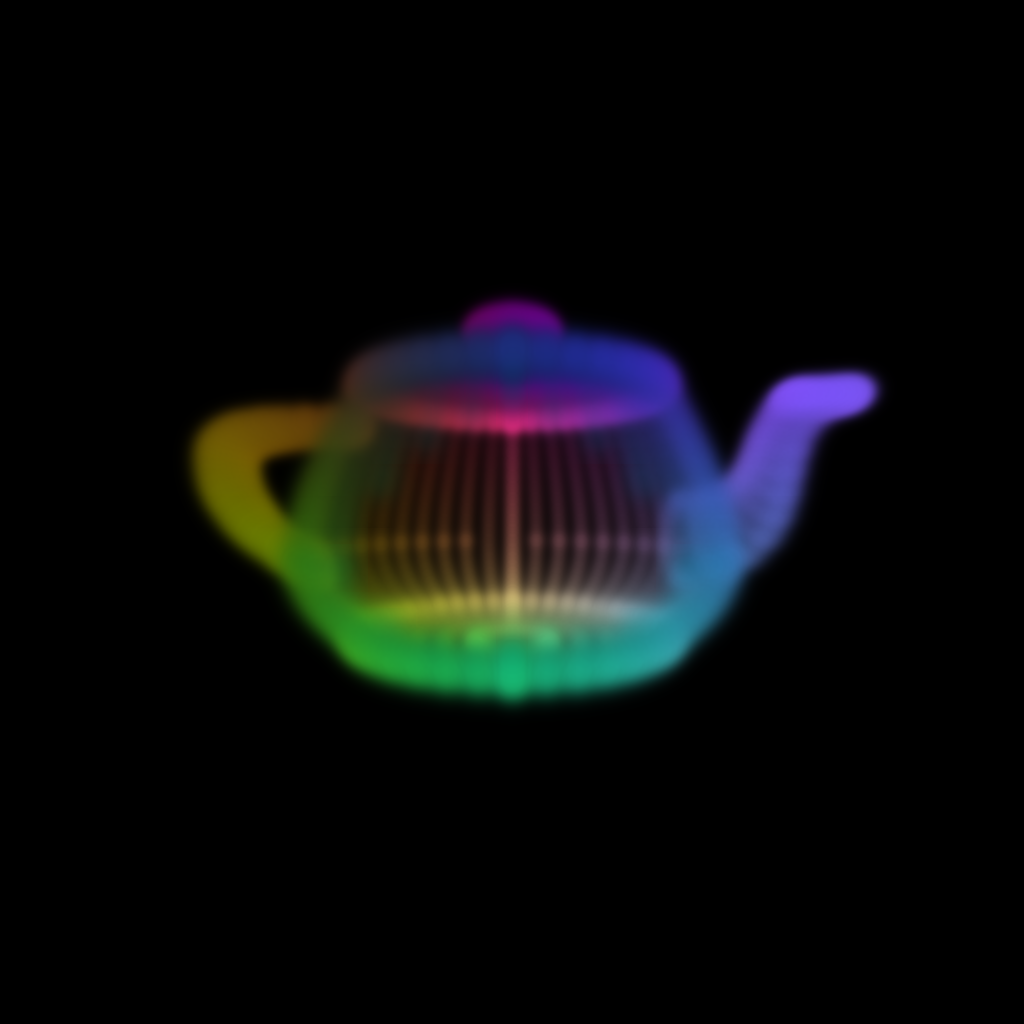
\includegraphics[scale=.2]{images/teapot.png}
        \caption{Teapot rendered using renderer from Section~\ref{sec:renderer}}
        \label{fig:teapot_render}
    \end{figure}

    \subsection{Dense Cube}
    Runtime averaged over 10 frames
    \begin{figure}[t]
        \centering
        
\includegraphics[scale=.2]{images/cube.png}
        \caption{Dense cube rendered using renderer from Section~\ref{sec:renderer}}
        \label{fig:cube_render}
    \end{figure}
    
    \chapter{Results and Discussion}

    The results of the experiments discussed in Chapter~\ref{ch:experiments} show

    \section{Runtime}

    On average the runtime is reduced by $19\%$ when compiling with clang instead of GCC.
    Rendering finishes about $9.4$ times faster when using tiling.

    Figure~\ref{fig:runtimes_st_simd_speedup} shows
    the speedups gained from employing the \gls{simd} routines described in Chapter~\ref{ch:optimizations}
    and Chapter~\ref{ch:implementation}. Showing a speedup of up to $25$ times when
    parallelization over the images pixels.
    \begin{figure}[t]
        \centering
        % Recommended preamble:
% \usetikzlibrary{arrows.meta}
% \usetikzlibrary{backgrounds}
% \usepgfplotslibrary{patchplots}
% \usepgfplotslibrary{fillbetween}
% \pgfplotsset{%
%     layers/standard/.define layer set={%
%         background,axis background,axis grid,axis ticks,axis lines,axis tick labels,pre main,main,axis descriptions,axis foreground%
%     }{
%         grid style={/pgfplots/on layer=axis grid},%
%         tick style={/pgfplots/on layer=axis ticks},%
%         axis line style={/pgfplots/on layer=axis lines},%
%         label style={/pgfplots/on layer=axis descriptions},%
%         legend style={/pgfplots/on layer=axis descriptions},%
%         title style={/pgfplots/on layer=axis descriptions},%
%         colorbar style={/pgfplots/on layer=axis descriptions},%
%         ticklabel style={/pgfplots/on layer=axis tick labels},%
%         axis background@ style={/pgfplots/on layer=axis background},%
%         3d box foreground style={/pgfplots/on layer=axis foreground},%
%     },
% }

\begin{tikzpicture}[/tikz/background rectangle/.style={fill={rgb,1:red,1.0;green,1.0;blue,1.0}, fill opacity={1.0}, draw opacity={1.0}}, show background rectangle, trim axis left]
\begin{axis}[point meta max={nan}, point meta min={nan}, legend cell align={left}, legend columns={1}, title={}, title style={at={{(0.5,1)}}, anchor={south}, font={{\fontsize{14 pt}{18.2 pt}\selectfont}}, color={rgb,1:red,0.0;green,0.0;blue,0.0}, draw opacity={1.0}, rotate={0.0}, align={center}}, legend style={color={rgb,1:red,0.0;green,0.0;blue,0.0}, draw opacity={1.0}, line width={1}, solid, fill={rgb,1:red,1.0;green,1.0;blue,1.0}, fill opacity={1.0}, text opacity={1.0}, font={{\fontsize{8 pt}{10.4 pt}\selectfont}}, text={rgb,1:red,0.0;green,0.0;blue,0.0}, cells={anchor={center}}, at={(1.02, 1)}, anchor={north west}}, axis background/.style={fill={rgb,1:red,1.0;green,1.0;blue,1.0}, opacity={1.0}}, anchor={north west}, xshift={1.0mm}, yshift={-1.0mm}, width=\textwidth, height=0.65*\textwidth, scaled x ticks={false}, xlabel={SIMD Variant}, x tick style={color={rgb,1:red,0.0;green,0.0;blue,0.0}, opacity={1.0}}, x tick label style={color={rgb,1:red,0.0;green,0.0;blue,0.0}, opacity={1.0}, rotate={0}}, xlabel style={at={(ticklabel cs:0.5)}, anchor=near ticklabel, at={{(ticklabel cs:0.5)}}, anchor={near ticklabel}, font={{\fontsize{11 pt}{14.3 pt}\selectfont}}, color={rgb,1:red,0.0;green,0.0;blue,0.0}, draw opacity={1.0}, rotate={0.0}}, xmajorgrids={true}, xmin={0.4099999999999999}, xmax={3.59}, xticklabels={{seq,transmittance,radiance,pixels}}, xtick={{0.5,1.5,2.5,3.5}}, xtick align={inside}, xticklabel style={font={{\fontsize{8 pt}{10.4 pt}\selectfont}}, color={rgb,1:red,0.0;green,0.0;blue,0.0}, draw opacity={1.0}, rotate={0.0}}, x grid style={color={rgb,1:red,0.0;green,0.0;blue,0.0}, draw opacity={0.1}, line width={0.5}, solid}, axis x line*={left}, x axis line style={color={rgb,1:red,0.0;green,0.0;blue,0.0}, draw opacity={1.0}, line width={1}, solid}, scaled y ticks={false}, ylabel={speedup}, y tick style={color={rgb,1:red,0.0;green,0.0;blue,0.0}, opacity={1.0}}, y tick label style={color={rgb,1:red,0.0;green,0.0;blue,0.0}, opacity={1.0}, rotate={0}}, ylabel style={at={(ticklabel cs:0.5)}, anchor=near ticklabel, at={{(ticklabel cs:0.5)}}, anchor={near ticklabel}, font={{\fontsize{11 pt}{14.3 pt}\selectfont}}, color={rgb,1:red,0.0;green,0.0;blue,0.0}, draw opacity={1.0}, rotate={0.0}}, ymajorgrids={true}, ymin={0.24697985042671178}, ymax={26.85369180201619}, yticklabels={{$5$,$10$,$15$,$20$,$25$}}, ytick={{5.0,10.0,15.0,20.0,25.0}}, ytick align={inside}, yticklabel style={font={{\fontsize{8 pt}{10.4 pt}\selectfont}}, color={rgb,1:red,0.0;green,0.0;blue,0.0}, draw opacity={1.0}, rotate={0.0}}, y grid style={color={rgb,1:red,0.0;green,0.0;blue,0.0}, draw opacity={0.1}, line width={0.5}, solid}, axis y line*={left}, y axis line style={color={rgb,1:red,0.0;green,0.0;blue,0.0}, draw opacity={1.0}, line width={1}, solid}, colorbar={false}]
    \addplot[color={rgb,1:red,0.0;green,0.6056;blue,0.9787}, name path={5bf36315-bcd1-444a-a57a-3e1ad204c3b5}, draw opacity={1.0}, line width={1}, solid, mark={*}, mark size={3.0 pt}, mark repeat={1}, mark options={color={rgb,1:red,0.0;green,0.0;blue,0.0}, draw opacity={0.0}, fill={rgb,1:red,0.0;green,0.6056;blue,0.9787}, fill opacity={1.0}, line width={0.0}, rotate={0}, solid}]
        table[row sep={\\}]
        {
            \\
            0.5  1.0  \\
            1.5  16.574272246776374  \\
            2.5  24.187207610406492  \\
            3.5  26.1006716524429  \\
        }
        ;
\end{axis}
\end{tikzpicture}

        \caption{Single Threaded Speedups from using SIMD}
        \label{fig:runtimes_st_simd_speedup}
    \end{figure}

    While the SVML routines provide much higher accuracy using them is not worth the
    performance trade-off as seen in Figure~\ref{fig:runtimes_st_svml_v_no}.
    \begin{figure}[t]
        \centering
        % Recommended preamble:
% \usetikzlibrary{arrows.meta}
% \usetikzlibrary{backgrounds}
% \usepgfplotslibrary{patchplots}
% \usepgfplotslibrary{fillbetween}
% \pgfplotsset{%
%     layers/standard/.define layer set={%
%         background,axis background,axis grid,axis ticks,axis lines,axis tick labels,pre main,main,axis descriptions,axis foreground%
%     }{
%         grid style={/pgfplots/on layer=axis grid},%
%         tick style={/pgfplots/on layer=axis ticks},%
%         axis line style={/pgfplots/on layer=axis lines},%
%         label style={/pgfplots/on layer=axis descriptions},%
%         legend style={/pgfplots/on layer=axis descriptions},%
%         title style={/pgfplots/on layer=axis descriptions},%
%         colorbar style={/pgfplots/on layer=axis descriptions},%
%         ticklabel style={/pgfplots/on layer=axis tick labels},%
%         axis background@ style={/pgfplots/on layer=axis background},%
%         3d box foreground style={/pgfplots/on layer=axis foreground},%
%     },
% }

\begin{tikzpicture}[/tikz/background rectangle/.style={fill={rgb,1:red,1.0;green,1.0;blue,1.0}, fill opacity={1.0}, draw opacity={1.0}}, show background rectangle, trim axis left]
\begin{axis}[point meta max={nan}, point meta min={nan}, legend cell align={left}, legend columns={1}, title={}, title style={at={{(0.5,1)}}, anchor={south}, font={{\fontsize{14 pt}{18.2 pt}\selectfont}}, color={rgb,1:red,0.0;green,0.0;blue,0.0}, draw opacity={1.0}, rotate={0.0}, align={center}}, legend style={color={rgb,1:red,0.0;green,0.0;blue,0.0}, draw opacity={1.0}, line width={1}, solid, fill={rgb,1:red,1.0;green,1.0;blue,1.0}, fill opacity={1.0}, text opacity={1.0}, font={{\fontsize{8 pt}{10.4 pt}\selectfont}}, text={rgb,1:red,0.0;green,0.0;blue,0.0}, cells={anchor={center}}, at={(0.98, 0.98)}, anchor={north east}}, axis background/.style={fill={rgb,1:red,1.0;green,1.0;blue,1.0}, opacity={1.0}}, anchor={north west}, xshift={1.0mm}, yshift={-1.0mm}, width=\textwidth, height=0.65*\textwidth, scaled x ticks={false}, xlabel={mode}, x tick style={color={rgb,1:red,0.0;green,0.0;blue,0.0}, opacity={1.0}}, x tick label style={color={rgb,1:red,0.0;green,0.0;blue,0.0}, opacity={1.0}, rotate={0}}, xlabel style={at={(ticklabel cs:0.5)}, anchor=near ticklabel, at={{(ticklabel cs:0.5)}}, anchor={near ticklabel}, font={{\fontsize{11 pt}{14.3 pt}\selectfont}}, color={rgb,1:red,0.0;green,0.0;blue,0.0}, draw opacity={1.0}, rotate={0.0}}, xmajorgrids={true}, xmin={-0.24572000000000127}, xmax={6.245720000000001}, xticklabels={{2,3,4,6,7,8}}, xtick={{0.5,1.5,2.5,3.5,4.5,5.5}}, xtick align={inside}, xticklabel style={font={{\fontsize{8 pt}{10.4 pt}\selectfont}}, color={rgb,1:red,0.0;green,0.0;blue,0.0}, draw opacity={1.0}, rotate={0.0}}, x grid style={color={rgb,1:red,0.0;green,0.0;blue,0.0}, draw opacity={0.1}, line width={0.5}, solid}, axis x line*={left}, x axis line style={color={rgb,1:red,0.0;green,0.0;blue,0.0}, draw opacity={1.0}, line width={1}, solid}, scaled y ticks={false}, ylabel={sec}, y tick style={color={rgb,1:red,0.0;green,0.0;blue,0.0}, opacity={1.0}}, y tick label style={color={rgb,1:red,0.0;green,0.0;blue,0.0}, opacity={1.0}, rotate={0}}, ylabel style={at={(ticklabel cs:0.5)}, anchor=near ticklabel, at={{(ticklabel cs:0.5)}}, anchor={near ticklabel}, font={{\fontsize{11 pt}{14.3 pt}\selectfont}}, color={rgb,1:red,0.0;green,0.0;blue,0.0}, draw opacity={1.0}, rotate={0.0}}, ymajorgrids={true}, ymin={0}, ymax={160}, yticklabels={{$0$,$50$,$100$,$150$}}, ytick={{0.0,50.0,100.0,150.0}}, ytick align={inside}, yticklabel style={font={{\fontsize{8 pt}{10.4 pt}\selectfont}}, color={rgb,1:red,0.0;green,0.0;blue,0.0}, draw opacity={1.0}, rotate={0.0}}, y grid style={color={rgb,1:red,0.0;green,0.0;blue,0.0}, draw opacity={0.1}, line width={0.5}, solid}, axis y line*={left}, y axis line style={color={rgb,1:red,0.0;green,0.0;blue,0.0}, draw opacity={1.0}, line width={1}, solid}, colorbar={false}]
    \addplot[color={rgb,1:red,0.0;green,0.0;blue,0.0}, name path={c86b5195-00a6-46cb-8b94-a5abf87928c2}, area legend, fill={rgb,1:red,0.0;green,0.6056;blue,0.9787}, fill opacity={1.0}, draw opacity={1.0}, line width={1}, solid]
        table[row sep={\\}]
        {
            \\
            0.09999999999999998  82.85655499999999  \\
            0.09999999999999998  0.0  \\
            0.5  0.0  \\
            0.5  82.85655499999999  \\
            0.09999999999999998  82.85655499999999  \\
        }
        ;
    \addlegendentry {No SVML}
    \addplot[color={rgb,1:red,0.0;green,0.0;blue,0.0}, name path={c86b5195-00a6-46cb-8b94-a5abf87928c2}, area legend, fill={rgb,1:red,0.0;green,0.6056;blue,0.9787}, fill opacity={1.0}, draw opacity={1.0}, line width={1}, solid, forget plot]
        table[row sep={\\}]
        {
            \\
            1.1  56.777414  \\
            1.1  0.0  \\
            1.5  0.0  \\
            1.5  56.777414  \\
            1.1  56.777414  \\
        }
        ;
    \addplot[color={rgb,1:red,0.0;green,0.0;blue,0.0}, name path={c86b5195-00a6-46cb-8b94-a5abf87928c2}, area legend, fill={rgb,1:red,0.0;green,0.6056;blue,0.9787}, fill opacity={1.0}, draw opacity={1.0}, line width={1}, solid, forget plot]
        table[row sep={\\}]
        {
            \\
            2.1  52.615010000000005  \\
            2.1  0.0  \\
            2.5000000000000004  0.0  \\
            2.5000000000000004  52.615010000000005  \\
            2.1  52.615010000000005  \\
        }
        ;
    \addplot[color={rgb,1:red,0.0;green,0.0;blue,0.0}, name path={c86b5195-00a6-46cb-8b94-a5abf87928c2}, area legend, fill={rgb,1:red,0.0;green,0.6056;blue,0.9787}, fill opacity={1.0}, draw opacity={1.0}, line width={1}, solid, forget plot]
        table[row sep={\\}]
        {
            \\
            3.1  9.692071  \\
            3.1  0.0  \\
            3.5000000000000004  0.0  \\
            3.5000000000000004  9.692071  \\
            3.1  9.692071  \\
        }
        ;
    \addplot[color={rgb,1:red,0.0;green,0.0;blue,0.0}, name path={c86b5195-00a6-46cb-8b94-a5abf87928c2}, area legend, fill={rgb,1:red,0.0;green,0.6056;blue,0.9787}, fill opacity={1.0}, draw opacity={1.0}, line width={1}, solid, forget plot]
        table[row sep={\\}]
        {
            \\
            4.1  5.829655300000001  \\
            4.1  0.0  \\
            4.5  0.0  \\
            4.5  5.829655300000001  \\
            4.1  5.829655300000001  \\
        }
        ;
    \addplot[color={rgb,1:red,0.0;green,0.0;blue,0.0}, name path={c86b5195-00a6-46cb-8b94-a5abf87928c2}, area legend, fill={rgb,1:red,0.0;green,0.6056;blue,0.9787}, fill opacity={1.0}, draw opacity={1.0}, line width={1}, solid, forget plot]
        table[row sep={\\}]
        {
            \\
            5.1  5.609189000000001  \\
            5.1  0.0  \\
            5.5  0.0  \\
            5.5  5.609189000000001  \\
            5.1  5.609189000000001  \\
        }
        ;
    \addplot[color={rgb,1:red,0.0;green,0.6056;blue,0.9787}, name path={1926d9c5-baf1-4dc3-9dae-31b0fc4fabe5}, only marks, draw opacity={1.0}, line width={0}, solid, mark={*}, mark size={0.0 pt}, mark repeat={1}, mark options={color={rgb,1:red,0.0;green,0.0;blue,0.0}, draw opacity={0.0}, fill={rgb,1:red,0.0;green,0.6056;blue,0.9787}, fill opacity={0.0}, line width={0.75}, rotate={0}, solid}, forget plot]
        table[row sep={\\}]
        {
            \\
            0.3  82.85655499999999  \\
            1.3  56.777414  \\
            2.3000000000000003  52.615010000000005  \\
            3.3000000000000003  9.692071  \\
            4.3  5.829655300000001  \\
            5.3  5.609189000000001  \\
        }
        ;
    \addplot[color={rgb,1:red,0.0;green,0.0;blue,0.0}, name path={86b6aa5d-4444-44d2-98ca-e8168ebb3c1e}, area legend, fill={rgb,1:red,0.8889;green,0.4356;blue,0.2781}, fill opacity={1.0}, draw opacity={1.0}, line width={1}, solid]
        table[row sep={\\}]
        {
            \\
            0.49999999999999994  150.07603  \\
            0.49999999999999994  0.0  \\
            0.8999999999999999  0.0  \\
            0.8999999999999999  150.07603  \\
            0.49999999999999994  150.07603  \\
        }
        ;
    \addlegendentry {SVML}
    \addplot[color={rgb,1:red,0.0;green,0.0;blue,0.0}, name path={86b6aa5d-4444-44d2-98ca-e8168ebb3c1e}, area legend, fill={rgb,1:red,0.8889;green,0.4356;blue,0.2781}, fill opacity={1.0}, draw opacity={1.0}, line width={1}, solid, forget plot]
        table[row sep={\\}]
        {
            \\
            1.5000000000000002  134.3319  \\
            1.5000000000000002  0.0  \\
            1.9000000000000001  0.0  \\
            1.9000000000000001  134.3319  \\
            1.5000000000000002  134.3319  \\
        }
        ;
    \addplot[color={rgb,1:red,0.0;green,0.0;blue,0.0}, name path={86b6aa5d-4444-44d2-98ca-e8168ebb3c1e}, area legend, fill={rgb,1:red,0.8889;green,0.4356;blue,0.2781}, fill opacity={1.0}, draw opacity={1.0}, line width={1}, solid, forget plot]
        table[row sep={\\}]
        {
            \\
            2.5  136.41681  \\
            2.5  0.0  \\
            2.9000000000000004  0.0  \\
            2.9000000000000004  136.41681  \\
            2.5  136.41681  \\
        }
        ;
    \addplot[color={rgb,1:red,0.0;green,0.0;blue,0.0}, name path={86b6aa5d-4444-44d2-98ca-e8168ebb3c1e}, area legend, fill={rgb,1:red,0.8889;green,0.4356;blue,0.2781}, fill opacity={1.0}, draw opacity={1.0}, line width={1}, solid, forget plot]
        table[row sep={\\}]
        {
            \\
            3.5  17.795441  \\
            3.5  0.0  \\
            3.9000000000000004  0.0  \\
            3.9000000000000004  17.795441  \\
            3.5  17.795441  \\
        }
        ;
    \addplot[color={rgb,1:red,0.0;green,0.0;blue,0.0}, name path={86b6aa5d-4444-44d2-98ca-e8168ebb3c1e}, area legend, fill={rgb,1:red,0.8889;green,0.4356;blue,0.2781}, fill opacity={1.0}, draw opacity={1.0}, line width={1}, solid, forget plot]
        table[row sep={\\}]
        {
            \\
            4.5  14.818772999999998  \\
            4.5  0.0  \\
            4.9  0.0  \\
            4.9  14.818772999999998  \\
            4.5  14.818772999999998  \\
        }
        ;
    \addplot[color={rgb,1:red,0.0;green,0.0;blue,0.0}, name path={86b6aa5d-4444-44d2-98ca-e8168ebb3c1e}, area legend, fill={rgb,1:red,0.8889;green,0.4356;blue,0.2781}, fill opacity={1.0}, draw opacity={1.0}, line width={1}, solid, forget plot]
        table[row sep={\\}]
        {
            \\
            5.5  15.021628  \\
            5.5  0.0  \\
            5.9  0.0  \\
            5.9  15.021628  \\
            5.5  15.021628  \\
        }
        ;
    \addplot[color={rgb,1:red,0.8889;green,0.4356;blue,0.2781}, name path={3d9a4735-6774-4b76-b169-138aa701b272}, only marks, draw opacity={1.0}, line width={0}, solid, mark={*}, mark size={0.0 pt}, mark repeat={1}, mark options={color={rgb,1:red,0.0;green,0.0;blue,0.0}, draw opacity={0.0}, fill={rgb,1:red,0.8889;green,0.4356;blue,0.2781}, fill opacity={0.0}, line width={0.75}, rotate={0}, solid}, forget plot]
        table[row sep={\\}]
        {
            \\
            0.7  150.07603  \\
            1.7000000000000002  134.3319  \\
            2.7  136.41681  \\
            3.7  17.795441  \\
            4.7  14.818772999999998  \\
            5.7  15.021628  \\
        }
        ;
\end{axis}
\end{tikzpicture}

        \caption{Single Threaded Runtimes using SVML and no SVML with Clang}
        \label{fig:runtimes_st_svml_v_no}
    \end{figure}

    \begin{figure}[t]
        \centering
        % Recommended preamble:
% \usetikzlibrary{arrows.meta}
% \usetikzlibrary{backgrounds}
% \usepgfplotslibrary{patchplots}
% \usepgfplotslibrary{fillbetween}
% \pgfplotsset{%
%     layers/standard/.define layer set={%
%         background,axis background,axis grid,axis ticks,axis lines,axis tick labels,pre main,main,axis descriptions,axis foreground%
%     }{
%         grid style={/pgfplots/on layer=axis grid},%
%         tick style={/pgfplots/on layer=axis ticks},%
%         axis line style={/pgfplots/on layer=axis lines},%
%         label style={/pgfplots/on layer=axis descriptions},%
%         legend style={/pgfplots/on layer=axis descriptions},%
%         title style={/pgfplots/on layer=axis descriptions},%
%         colorbar style={/pgfplots/on layer=axis descriptions},%
%         ticklabel style={/pgfplots/on layer=axis tick labels},%
%         axis background@ style={/pgfplots/on layer=axis background},%
%         3d box foreground style={/pgfplots/on layer=axis foreground},%
%     },
% }

\begin{tikzpicture}[/tikz/background rectangle/.style={fill={rgb,1:red,1.0;green,1.0;blue,1.0}, fill opacity={1.0}, draw opacity={1.0}}, show background rectangle, trim axis left]
\begin{axis}[point meta max={nan}, point meta min={nan}, legend cell align={left}, legend columns={1}, title={}, title style={at={{(0.5,1)}}, anchor={south}, font={{\fontsize{14 pt}{18.2 pt}\selectfont}}, color={rgb,1:red,0.0;green,0.0;blue,0.0}, draw opacity={1.0}, rotate={0.0}, align={center}}, legend style={color={rgb,1:red,0.0;green,0.0;blue,0.0}, draw opacity={1.0}, line width={1}, solid, fill={rgb,1:red,1.0;green,1.0;blue,1.0}, fill opacity={1.0}, text opacity={1.0}, font={{\fontsize{8 pt}{10.4 pt}\selectfont}}, text={rgb,1:red,0.0;green,0.0;blue,0.0}, cells={anchor={center}}, at={(0.02, 0.98)}, anchor={north west}}, axis background/.style={fill={rgb,1:red,1.0;green,1.0;blue,1.0}, opacity={1.0}}, anchor={north west}, xshift={1.0mm}, yshift={-1.0mm}, width=\textwidth, height=0.65*\textwidth, scaled x ticks={false}, xlabel={mode}, x tick style={color={rgb,1:red,0.0;green,0.0;blue,0.0}, opacity={1.0}}, x tick label style={color={rgb,1:red,0.0;green,0.0;blue,0.0}, opacity={1.0}, rotate={0}}, xlabel style={at={(ticklabel cs:0.5)}, anchor=near ticklabel, at={{(ticklabel cs:0.5)}}, anchor={near ticklabel}, font={{\fontsize{11 pt}{14.3 pt}\selectfont}}, color={rgb,1:red,0.0;green,0.0;blue,0.0}, draw opacity={1.0}, rotate={0.0}}, xmajorgrids={true}, xmin={-0.12211999999999978}, xmax={4.122120000000001}, xticklabels={{5,6,7,8}}, xtick={{0.5,1.5,2.5,3.5}}, xtick align={inside}, xticklabel style={font={{\fontsize{8 pt}{10.4 pt}\selectfont}}, color={rgb,1:red,0.0;green,0.0;blue,0.0}, draw opacity={1.0}, rotate={0.0}}, x grid style={color={rgb,1:red,0.0;green,0.0;blue,0.0}, draw opacity={0.1}, line width={0.5}, solid}, axis x line*={left}, x axis line style={color={rgb,1:red,0.0;green,0.0;blue,0.0}, draw opacity={1.0}, line width={1}, solid}, scaled y ticks={false}, ylabel={speedup}, y tick style={color={rgb,1:red,0.0;green,0.0;blue,0.0}, opacity={1.0}}, y tick label style={color={rgb,1:red,0.0;green,0.0;blue,0.0}, opacity={1.0}, rotate={0}}, ylabel style={at={(ticklabel cs:0.5)}, anchor=near ticklabel, at={{(ticklabel cs:0.5)}}, anchor={near ticklabel}, font={{\fontsize{11 pt}{14.3 pt}\selectfont}}, color={rgb,1:red,0.0;green,0.0;blue,0.0}, draw opacity={1.0}, rotate={0.0}}, ymode={log}, log basis y={10}, ymajorgrids={true}, ymin={0.1}, ymax={1000}, yticklabels={{$10^{-1}$,$10^{0}$,$10^{1}$,$10^{2}$,$10^{3}$}}, ytick={{0.1,1.0,10.0,100.0,1000.0}}, ytick align={inside}, yticklabel style={font={{\fontsize{8 pt}{10.4 pt}\selectfont}}, color={rgb,1:red,0.0;green,0.0;blue,0.0}, draw opacity={1.0}, rotate={0.0}}, y grid style={color={rgb,1:red,0.0;green,0.0;blue,0.0}, draw opacity={0.1}, line width={0.5}, solid}, axis y line*={left}, y axis line style={color={rgb,1:red,0.0;green,0.0;blue,0.0}, draw opacity={1.0}, line width={1}, solid}, colorbar={false}]
    \addplot[color={rgb,1:red,0.0;green,0.0;blue,0.0}, name path={6e981cd9-85b2-4ee6-8719-361675bb9514}, area legend, fill={rgb,1:red,0.0;green,0.6056;blue,0.9787}, fill opacity={1.0}, draw opacity={1.0}, line width={1}, solid]
        table[row sep={\\}]
        {
            \\
            0.09999999999999998  23.65444567567838  \\
            0.09999999999999998  0.01  \\
            0.5  0.01  \\
            0.5  23.65444567567838  \\
            0.09999999999999998  23.65444567567838  \\
        }
        ;
    \addlegendentry {Multi Threaded (32)}
    \addplot[color={rgb,1:red,0.0;green,0.0;blue,0.0}, name path={6e981cd9-85b2-4ee6-8719-361675bb9514}, area legend, fill={rgb,1:red,0.0;green,0.6056;blue,0.9787}, fill opacity={1.0}, draw opacity={1.0}, line width={1}, solid, forget plot]
        table[row sep={\\}]
        {
            \\
            1.1  265.5680082246698  \\
            1.1  0.01  \\
            1.5  0.01  \\
            1.5  265.5680082246698  \\
            1.1  265.5680082246698  \\
        }
        ;
    \addplot[color={rgb,1:red,0.0;green,0.0;blue,0.0}, name path={6e981cd9-85b2-4ee6-8719-361675bb9514}, area legend, fill={rgb,1:red,0.0;green,0.6056;blue,0.9787}, fill opacity={1.0}, draw opacity={1.0}, line width={1}, solid, forget plot]
        table[row sep={\\}]
        {
            \\
            2.1  355.7049944202922  \\
            2.1  0.01  \\
            2.5000000000000004  0.01  \\
            2.5000000000000004  355.7049944202922  \\
            2.1  355.7049944202922  \\
        }
        ;
    \addplot[color={rgb,1:red,0.0;green,0.0;blue,0.0}, name path={6e981cd9-85b2-4ee6-8719-361675bb9514}, area legend, fill={rgb,1:red,0.0;green,0.6056;blue,0.9787}, fill opacity={1.0}, draw opacity={1.0}, line width={1}, solid, forget plot]
        table[row sep={\\}]
        {
            \\
            3.1  367.4140587599766  \\
            3.1  0.01  \\
            3.5000000000000004  0.01  \\
            3.5000000000000004  367.4140587599766  \\
            3.1  367.4140587599766  \\
        }
        ;
    \addplot[color={rgb,1:red,0.0;green,0.6056;blue,0.9787}, name path={a013573c-c316-4ece-9d95-19605d00befc}, only marks, draw opacity={1.0}, line width={0}, solid, mark={*}, mark size={0.0 pt}, mark repeat={1}, mark options={color={rgb,1:red,0.0;green,0.0;blue,0.0}, draw opacity={0.0}, fill={rgb,1:red,0.0;green,0.6056;blue,0.9787}, fill opacity={0.0}, line width={0.75}, rotate={0}, solid}, forget plot]
        table[row sep={\\}]
        {
            \\
            0.3  23.65444567567838  \\
            1.3  265.5680082246698  \\
            2.3000000000000003  355.7049944202922  \\
            3.3000000000000003  367.4140587599766  \\
        }
        ;
    \addplot[color={rgb,1:red,0.0;green,0.0;blue,0.0}, name path={d6331eff-feec-409a-b534-63927c3fb3c2}, area legend, fill={rgb,1:red,0.8889;green,0.4356;blue,0.2781}, fill opacity={1.0}, draw opacity={1.0}, line width={1}, solid]
        table[row sep={\\}]
        {
            \\
            0.49999999999999994  1.0  \\
            0.49999999999999994  0.01  \\
            0.8999999999999999  0.01  \\
            0.8999999999999999  1.0  \\
            0.49999999999999994  1.0  \\
        }
        ;
    \addlegendentry {Single Threaded}
    \addplot[color={rgb,1:red,0.0;green,0.0;blue,0.0}, name path={d6331eff-feec-409a-b534-63927c3fb3c2}, area legend, fill={rgb,1:red,0.8889;green,0.4356;blue,0.2781}, fill opacity={1.0}, draw opacity={1.0}, line width={1}, solid, forget plot]
        table[row sep={\\}]
        {
            \\
            1.5000000000000002  14.382101757091117  \\
            1.5000000000000002  0.01  \\
            1.9000000000000001  0.01  \\
            1.9000000000000001  14.382101757091117  \\
            1.5000000000000002  14.382101757091117  \\
        }
        ;
    \addplot[color={rgb,1:red,0.0;green,0.0;blue,0.0}, name path={d6331eff-feec-409a-b534-63927c3fb3c2}, area legend, fill={rgb,1:red,0.8889;green,0.4356;blue,0.2781}, fill opacity={1.0}, draw opacity={1.0}, line width={1}, solid, forget plot]
        table[row sep={\\}]
        {
            \\
            2.5  23.446212705235347  \\
            2.5  0.01  \\
            2.9000000000000004  0.01  \\
            2.9000000000000004  23.446212705235347  \\
            2.5  23.446212705235347  \\
        }
        ;
    \addplot[color={rgb,1:red,0.0;green,0.0;blue,0.0}, name path={d6331eff-feec-409a-b534-63927c3fb3c2}, area legend, fill={rgb,1:red,0.8889;green,0.4356;blue,0.2781}, fill opacity={1.0}, draw opacity={1.0}, line width={1}, solid, forget plot]
        table[row sep={\\}]
        {
            \\
            3.5  23.78870138617995  \\
            3.5  0.01  \\
            3.9000000000000004  0.01  \\
            3.9000000000000004  23.78870138617995  \\
            3.5  23.78870138617995  \\
        }
        ;
    \addplot[color={rgb,1:red,0.8889;green,0.4356;blue,0.2781}, name path={a6896615-971e-49c6-b154-c0da664a0694}, only marks, draw opacity={1.0}, line width={0}, solid, mark={*}, mark size={0.0 pt}, mark repeat={1}, mark options={color={rgb,1:red,0.0;green,0.0;blue,0.0}, draw opacity={0.0}, fill={rgb,1:red,0.8889;green,0.4356;blue,0.2781}, fill opacity={0.0}, line width={0.75}, rotate={0}, solid}, forget plot]
        table[row sep={\\}]
        {
            \\
            0.7  1.0  \\
            1.7000000000000002  14.382101757091117  \\
            2.7  23.446212705235347  \\
            3.7  23.78870138617995  \\
        }
        ;
\end{axis}
\end{tikzpicture}

        \caption{Speedup of Modes 6-8 relative to Mode 5}
        \label{fig:runtimes_st_v_mt}
    \end{figure}

    \section{HPCTOOLKIT}
    \cite{hpc_toolkit}

    The derived metrics used were vector instruction waste and vector instruction efficiency defined as:
    \begin{align}
        \text{waste}(\text{cycles}, \text{instructions}) = 2 \cdot \text{cycles} - \text{instructions} \label{eq:vec_waste}\\
        \text{efficiency}(\text{cycles}, \text{instructions}) = 100 \cdot \frac{\text{instructions}}{2\cdot\text{cycles}} \label{eq:vec_efficiency}
    \end{align}
    which should be based on the exclusive\footnote{An exclusive metric refers to the quantity of the metric measured for that scope
    alone, disregarding nested scopes such as function calls. Reference: HPCTOOLKIT User Manual page 18
    \href{https://hpctoolkit.org/manual/HPCToolkit-users-manual.pdf}{https://hpctoolkit.org/manual/HPCToolkit-users-manual.pdf}}
    \mintinline{c}{PAPI_TOT_CYC} (total cycles) and \mintinline{c}{PAPI_VEC_INS}
    (vector instructions) metrics for the given scopes. HPCToolkit does not include inlined functions in exclusive metrics, which is why \gls{simd}
    instructions and CPU cycles generated by the T-SIMD library would not count towards the exclusive \mintinline{c}{PAPI_VEC_INS} and \mintinline{c}{PAPI_TOT_CYC}
    metrics.

    \begin{listing}[H]
        \begin{minted}[linenos, frame=lines]{c++}
f32 func(f32 in)
{
    // inlined broadcast should count for scope
    simd::Vec<simd::Float> x = simd::set1(in);
    // exp should not count for scope
    x = simd::exp(x);
    // inlined mul and broadcast should count for scope
    x = x * simd::set1(2.f);
    return x;
}
        \end{minted}
        \caption{Example for functions calls that should and should not count towards exclusive metrics.}
        \label{lst:scopes_example}
    \end{listing}

    As such the inclusive metrics are used for calculating the derived metrics. To get the exclusive derived metrics including the inlined T-SIMD functions I subtract
    the inclusive derived metrics of the functions I want to disregard. For the example in Listing~\ref{lst:scopes_example}
    this would be:
    \[ \text{metric}_e = \text{metric}_i - \text{metric}_{\text{simd::exp}} \]
    where $\text{metric}_i$ is the inclusive metric and $\text{matric}_{\text{simd::exp}}$ is the metric for the \mintinline{c++}{simd::exp} call.

    %Therefore the derived metrics are calculated using the inclusive metrics. To obtain the final value for the derived metrics the
    %value of the derived metrics of the scopes of non T-SIMD functions are subtracted from the value calculated using the inclusive metrics.

    \chapter{Conclusion and Future Work}
    %@TODO: Short recap + what can still be done: anisotropic Gaussians, loading models learned via Gaussian splatting, more efficient tiling method using SIMD, performance left on the table TBD (see results)
    \section{Conclusion}
    \begin{itemize}
        \item SIMD + Tiling lead to massive performance improvements
    \end{itemize}

    \section{Future Work}
    \begin{itemize}
        \item Memory/Cache Bottleneck?
        \item Anisotropic Gaussians
        \item Loading Scenes learned via Gaussian splatting
        \item More efficient tiling (SIMD, Threads)
        \item Combining Splatting and Ray Tracing
        \item GPU Implementation
    \end{itemize}

    \appendix
    \chapter{Tables}
    \label{ch:tables}
    \begin{table}[H]
        \centering
        \rowcolors{1}{white}{lightgray}
        \begin{tabular}{|c | c | c | c|}
            \hline
            Mode & GCC               & Clang & SVML\\\hline
            1 st & $\sim1648.17$ sec & $\sim1373.29$ sec & - \\
            2 st & $\sim96.47$ sec   & $\sim82.86$ sec   & $\sim150.08$ sec\\
            3 st & $\sim69.44$ sec   & $\sim56.78$ sec   & $\sim134.33$ sec\\
            4 st & $\sim67.19$ sec   & $\sim52.62$ sec   & $\sim136.42$ sec\\
            5 st & $\sim170.74$ sec  & $\sim136.84$ sec  & - \\
            6 st & $\sim11.95$ sec   & $\sim9.69$ sec    & $\sim17.80$ sec\\
            7 st & $\sim7.46$ sec    & $\sim5.83$ sec    & $\sim14.82$ sec\\
            8 st & $\sim7.08$ sec    & $\sim5.61$ sec    & $\sim15.02$ sec\\\hline\hline

            5 mt & $\sim6.60$ sec    & $\sim5.93$ sec    & $\sim5.94$ sec\\
            6 mt & $\sim0.62$ sec    & $\sim0.53$ sec    & $\sim0.95$ sec\\
            7 mt & $\sim0.47$ sec    & $\sim0.40$ sec    & $\sim0.80$ sec\\
            8 mt & $\sim0.45$ sec    & $\sim0.39$ sec    & $\sim0.78$ sec\\
            \hline
        \end{tabular}
        \caption{Runtime of rendering the dense cube based on compiler, SVML usage, and mode using AVX512. Averaged over 10 Frames.}
        \label{tab:perf_dense_cube_avx512}
    \end{table}

    \chapter{Figures}
    \begin{figure}[H]
        \centering
        % Recommended preamble:
% \usetikzlibrary{arrows.meta}
% \usetikzlibrary{backgrounds}
% \usepgfplotslibrary{patchplots}
% \usepgfplotslibrary{fillbetween}
% \pgfplotsset{%
%     layers/standard/.define layer set={%
%         background,axis background,axis grid,axis ticks,axis lines,axis tick labels,pre main,main,axis descriptions,axis foreground%
%     }{
%         grid style={/pgfplots/on layer=axis grid},%
%         tick style={/pgfplots/on layer=axis ticks},%
%         axis line style={/pgfplots/on layer=axis lines},%
%         label style={/pgfplots/on layer=axis descriptions},%
%         legend style={/pgfplots/on layer=axis descriptions},%
%         title style={/pgfplots/on layer=axis descriptions},%
%         colorbar style={/pgfplots/on layer=axis descriptions},%
%         ticklabel style={/pgfplots/on layer=axis tick labels},%
%         axis background@ style={/pgfplots/on layer=axis background},%
%         3d box foreground style={/pgfplots/on layer=axis foreground},%
%     },
% }

\begin{tikzpicture}[/tikz/background rectangle/.style={fill={rgb,1:red,1.0;green,1.0;blue,1.0}, fill opacity={1.0}, draw opacity={1.0}}, show background rectangle]
\begin{axis}[point meta max={nan}, point meta min={nan}, legend cell align={left}, legend columns={1}, title={}, title style={at={{(0.5,1)}}, anchor={south}, font={{\fontsize{14 pt}{18.2 pt}\selectfont}}, color={rgb,1:red,0.0;green,0.0;blue,0.0}, draw opacity={1.0}, rotate={0.0}, align={center}}, legend style={color={rgb,1:red,0.0;green,0.0;blue,0.0}, draw opacity={1.0}, line width={1}, solid, fill={rgb,1:red,1.0;green,1.0;blue,1.0}, fill opacity={1.0}, text opacity={1.0}, font={{\fontsize{8 pt}{10.4 pt}\selectfont}}, text={rgb,1:red,0.0;green,0.0;blue,0.0}, cells={anchor={center}}, at={(0.02, 0.98)}, anchor={north west}}, axis background/.style={fill={rgb,1:red,1.0;green,1.0;blue,1.0}, opacity={1.0}}, anchor={north west}, xshift={1.0mm}, yshift={-1.0mm}, width={150.4mm}, height={99.6mm}, scaled x ticks={false}, xlabel={}, x tick style={color={rgb,1:red,0.0;green,0.0;blue,0.0}, opacity={1.0}}, x tick label style={color={rgb,1:red,0.0;green,0.0;blue,0.0}, opacity={1.0}, rotate={0}}, xlabel style={at={(ticklabel cs:0.5)}, anchor=near ticklabel, at={{(ticklabel cs:0.5)}}, anchor={near ticklabel}, font={{\fontsize{11 pt}{14.3 pt}\selectfont}}, color={rgb,1:red,0.0;green,0.0;blue,0.0}, draw opacity={1.0}, rotate={0.0}}, xmajorgrids={true}, xmin={-0.18392000000000008}, xmax={5.1839200000000005}, xticklabels={{Abramowitz,SVML/STD,Spline,Spline Mirror,Taylor}}, xtick={{0.5,1.5,2.5,3.5,4.5}}, xtick align={inside}, xticklabel style={font={{\fontsize{8 pt}{10.4 pt}\selectfont}}, color={rgb,1:red,0.0;green,0.0;blue,0.0}, draw opacity={1.0}, rotate={0.0}}, x grid style={color={rgb,1:red,0.0;green,0.0;blue,0.0}, draw opacity={0.1}, line width={0.5}, solid}, axis x line*={left}, x axis line style={color={rgb,1:red,0.0;green,0.0;blue,0.0}, draw opacity={1.0}, line width={1}, solid}, scaled y ticks={false}, ylabel={avg. cycles}, y tick style={color={rgb,1:red,0.0;green,0.0;blue,0.0}, opacity={1.0}}, y tick label style={color={rgb,1:red,0.0;green,0.0;blue,0.0}, opacity={1.0}, rotate={0}}, ylabel style={at={(ticklabel cs:0.5)}, anchor=near ticklabel, at={{(ticklabel cs:0.5)}}, anchor={near ticklabel}, font={{\fontsize{11 pt}{14.3 pt}\selectfont}}, color={rgb,1:red,0.0;green,0.0;blue,0.0}, draw opacity={1.0}, rotate={0.0}}, ymajorgrids={true}, ymin={0.0}, ymax={61.355656}, yticklabels={{$0$,$10$,$20$,$30$,$40$,$50$,$60$}}, ytick={{0.0,10.0,20.0,30.0,40.0,50.0,60.0}}, ytick align={inside}, yticklabel style={font={{\fontsize{8 pt}{10.4 pt}\selectfont}}, color={rgb,1:red,0.0;green,0.0;blue,0.0}, draw opacity={1.0}, rotate={0.0}}, y grid style={color={rgb,1:red,0.0;green,0.0;blue,0.0}, draw opacity={0.1}, line width={0.5}, solid}, axis y line*={left}, y axis line style={color={rgb,1:red,0.0;green,0.0;blue,0.0}, draw opacity={1.0}, line width={1}, solid}, colorbar={false}]
    \addplot[color={rgb,1:red,0.0;green,0.0;blue,0.0}, name path={1}, area legend, fill={rgb,1:red,0.0;green,0.6056;blue,0.9787}, fill opacity={1.0}, draw opacity={1.0}, line width={1}, solid]
        table[row sep={\\}]
        {
            \\
            0.09999999999999998  2.495022  \\
            0.09999999999999998  0.0  \\
            0.5  0.0  \\
            0.5  2.495022  \\
            0.09999999999999998  2.495022  \\
        }
        ;
    \addlegendentry {SIMD}
    \addplot[color={rgb,1:red,0.0;green,0.0;blue,0.0}, name path={1}, area legend, fill={rgb,1:red,0.0;green,0.6056;blue,0.9787}, fill opacity={1.0}, draw opacity={1.0}, line width={1}, solid, forget plot]
        table[row sep={\\}]
        {
            \\
            1.1  5.6820583  \\
            1.1  0.0  \\
            1.5  0.0  \\
            1.5  5.6820583  \\
            1.1  5.6820583  \\
        }
        ;
    \addplot[color={rgb,1:red,0.0;green,0.0;blue,0.0}, name path={1}, area legend, fill={rgb,1:red,0.0;green,0.6056;blue,0.9787}, fill opacity={1.0}, draw opacity={1.0}, line width={1}, solid, forget plot]
        table[row sep={\\}]
        {
            \\
            2.1  4.1816087  \\
            2.1  0.0  \\
            2.5000000000000004  0.0  \\
            2.5000000000000004  4.1816087  \\
            2.1  4.1816087  \\
        }
        ;
    \addplot[color={rgb,1:red,0.0;green,0.0;blue,0.0}, name path={1}, area legend, fill={rgb,1:red,0.0;green,0.6056;blue,0.9787}, fill opacity={1.0}, draw opacity={1.0}, line width={1}, solid, forget plot]
        table[row sep={\\}]
        {
            \\
            3.1  3.3629444  \\
            3.1  0.0  \\
            3.5000000000000004  0.0  \\
            3.5000000000000004  3.3629444  \\
            3.1  3.3629444  \\
        }
        ;
    \addplot[color={rgb,1:red,0.0;green,0.0;blue,0.0}, name path={1}, area legend, fill={rgb,1:red,0.0;green,0.6056;blue,0.9787}, fill opacity={1.0}, draw opacity={1.0}, line width={1}, solid, forget plot]
        table[row sep={\\}]
        {
            \\
            4.1  2.6012878  \\
            4.1  0.0  \\
            4.5  0.0  \\
            4.5  2.6012878  \\
            4.1  2.6012878  \\
        }
        ;
    \addplot[color={rgb,1:red,0.0;green,0.6056;blue,0.9787}, name path={2}, only marks, draw opacity={1.0}, line width={0}, solid, mark={*}, mark size={0.0 pt}, mark repeat={1}, mark options={color={rgb,1:red,0.0;green,0.0;blue,0.0}, draw opacity={0.0}, fill={rgb,1:red,0.0;green,0.6056;blue,0.9787}, fill opacity={0.0}, line width={0.75}, rotate={0}, solid}, forget plot]
        table[row sep={\\}]
        {
            \\
            0.3  2.495022  \\
            1.3  5.6820583  \\
            2.3000000000000003  4.1816087  \\
            3.3000000000000003  3.3629444  \\
            4.3  2.6012878  \\
        }
        ;
    \addplot[color={rgb,1:red,0.0;green,0.0;blue,0.0}, name path={3}, area legend, fill={rgb,1:red,0.8889;green,0.4356;blue,0.2781}, fill opacity={1.0}, draw opacity={1.0}, line width={1}, solid]
        table[row sep={\\}]
        {
            \\
            0.49999999999999994  12.119275  \\
            0.49999999999999994  0.0  \\
            0.8999999999999999  0.0  \\
            0.8999999999999999  12.119275  \\
            0.49999999999999994  12.119275  \\
        }
        ;
    \addlegendentry {Sequential}
    \addplot[color={rgb,1:red,0.0;green,0.0;blue,0.0}, name path={3}, area legend, fill={rgb,1:red,0.8889;green,0.4356;blue,0.2781}, fill opacity={1.0}, draw opacity={1.0}, line width={1}, solid, forget plot]
        table[row sep={\\}]
        {
            \\
            1.5000000000000002  61.355656  \\
            1.5000000000000002  0.0  \\
            1.9000000000000001  0.0  \\
            1.9000000000000001  61.355656  \\
            1.5000000000000002  61.355656  \\
        }
        ;
    \addplot[color={rgb,1:red,0.0;green,0.0;blue,0.0}, name path={3}, area legend, fill={rgb,1:red,0.8889;green,0.4356;blue,0.2781}, fill opacity={1.0}, draw opacity={1.0}, line width={1}, solid, forget plot]
        table[row sep={\\}]
        {
            \\
            2.5  39.78879  \\
            2.5  0.0  \\
            2.9000000000000004  0.0  \\
            2.9000000000000004  39.78879  \\
            2.5  39.78879  \\
        }
        ;
    \addplot[color={rgb,1:red,0.0;green,0.0;blue,0.0}, name path={3}, area legend, fill={rgb,1:red,0.8889;green,0.4356;blue,0.2781}, fill opacity={1.0}, draw opacity={1.0}, line width={1}, solid, forget plot]
        table[row sep={\\}]
        {
            \\
            3.5  48.166466  \\
            3.5  0.0  \\
            3.9000000000000004  0.0  \\
            3.9000000000000004  48.166466  \\
            3.5  48.166466  \\
        }
        ;
    \addplot[color={rgb,1:red,0.0;green,0.0;blue,0.0}, name path={3}, area legend, fill={rgb,1:red,0.8889;green,0.4356;blue,0.2781}, fill opacity={1.0}, draw opacity={1.0}, line width={1}, solid, forget plot]
        table[row sep={\\}]
        {
            \\
            4.5  30.905552  \\
            4.5  0.0  \\
            4.9  0.0  \\
            4.9  30.905552  \\
            4.5  30.905552  \\
        }
        ;
    \addplot[color={rgb,1:red,0.8889;green,0.4356;blue,0.2781}, name path={4}, only marks, draw opacity={1.0}, line width={0}, solid, mark={*}, mark size={0.0 pt}, mark repeat={1}, mark options={color={rgb,1:red,0.0;green,0.0;blue,0.0}, draw opacity={0.0}, fill={rgb,1:red,0.8889;green,0.4356;blue,0.2781}, fill opacity={0.0}, line width={0.75}, rotate={0}, solid}, forget plot]
        table[row sep={\\}]
        {
            \\
            0.7  12.119275  \\
            1.7000000000000002  61.355656  \\
            2.7  39.78879  \\
            3.7  48.166466  \\
            4.7  30.905552  \\
        }
        ;
\end{axis}
\end{tikzpicture}

        \caption{Cycles to calculate $n$ values of $\erf$.}
    \end{figure}
    \begin{figure}[H]
        \centering
        % Recommended preamble:
% \usetikzlibrary{arrows.meta}
% \usetikzlibrary{backgrounds}
% \usepgfplotslibrary{patchplots}
% \usepgfplotslibrary{fillbetween}
% \pgfplotsset{%
%     layers/standard/.define layer set={%
%         background,axis background,axis grid,axis ticks,axis lines,axis tick labels,pre main,main,axis descriptions,axis foreground%
%     }{
%         grid style={/pgfplots/on layer=axis grid},%
%         tick style={/pgfplots/on layer=axis ticks},%
%         axis line style={/pgfplots/on layer=axis lines},%
%         label style={/pgfplots/on layer=axis descriptions},%
%         legend style={/pgfplots/on layer=axis descriptions},%
%         title style={/pgfplots/on layer=axis descriptions},%
%         colorbar style={/pgfplots/on layer=axis descriptions},%
%         ticklabel style={/pgfplots/on layer=axis tick labels},%
%         axis background@ style={/pgfplots/on layer=axis background},%
%         3d box foreground style={/pgfplots/on layer=axis foreground},%
%     },
% }

\begin{tikzpicture}[/tikz/background rectangle/.style={fill={rgb,1:red,1.0;green,1.0;blue,1.0}, fill opacity={1.0}, draw opacity={1.0}}, show background rectangle]
\begin{axis}[point meta max={nan}, point meta min={nan}, legend cell align={left}, legend columns={1}, title={}, title style={at={{(0.5,1)}}, anchor={south}, font={{\fontsize{14 pt}{18.2 pt}\selectfont}}, color={rgb,1:red,0.0;green,0.0;blue,0.0}, draw opacity={1.0}, rotate={0.0}, align={center}}, legend style={color={rgb,1:red,0.0;green,0.0;blue,0.0}, draw opacity={1.0}, line width={1}, solid, fill={rgb,1:red,1.0;green,1.0;blue,1.0}, fill opacity={1.0}, text opacity={1.0}, font={{\fontsize{8 pt}{10.4 pt}\selectfont}}, text={rgb,1:red,0.0;green,0.0;blue,0.0}, cells={anchor={center}}, at={(0.02, 0.98)}, anchor={north west}}, axis background/.style={fill={rgb,1:red,1.0;green,1.0;blue,1.0}, opacity={1.0}}, anchor={north west}, xshift={1.0mm}, yshift={-1.0mm}, width={150.4mm}, height={99.6mm}, scaled x ticks={false}, xlabel={}, x tick style={color={rgb,1:red,0.0;green,0.0;blue,0.0}, opacity={1.0}}, x tick label style={color={rgb,1:red,0.0;green,0.0;blue,0.0}, opacity={1.0}, rotate={0}}, xlabel style={at={(ticklabel cs:0.5)}, anchor=near ticklabel, at={{(ticklabel cs:0.5)}}, anchor={near ticklabel}, font={{\fontsize{11 pt}{14.3 pt}\selectfont}}, color={rgb,1:red,0.0;green,0.0;blue,0.0}, draw opacity={1.0}, rotate={0.0}}, xmajorgrids={true}, xmin={-0.11305999999999994}, xmax={3.8110600000000003}, xticklabels={{Fast,SVML/STD,Spline,VCL}}, xtick={{0.5,1.5,2.5,3.5}}, xtick align={inside}, xticklabel style={font={{\fontsize{8 pt}{10.4 pt}\selectfont}}, color={rgb,1:red,0.0;green,0.0;blue,0.0}, draw opacity={1.0}, rotate={0.0}}, x grid style={color={rgb,1:red,0.0;green,0.0;blue,0.0}, draw opacity={0.1}, line width={0.5}, solid}, axis x line*={left}, x axis line style={color={rgb,1:red,0.0;green,0.0;blue,0.0}, draw opacity={1.0}, line width={1}, solid}, scaled y ticks={false}, ylabel={avg. cycles}, y tick style={color={rgb,1:red,0.0;green,0.0;blue,0.0}, opacity={1.0}}, y tick label style={color={rgb,1:red,0.0;green,0.0;blue,0.0}, opacity={1.0}, rotate={0}}, ylabel style={at={(ticklabel cs:0.5)}, anchor=near ticklabel, at={{(ticklabel cs:0.5)}}, anchor={near ticklabel}, font={{\fontsize{11 pt}{14.3 pt}\selectfont}}, color={rgb,1:red,0.0;green,0.0;blue,0.0}, draw opacity={1.0}, rotate={0.0}}, ymajorgrids={true}, ymin={0.0}, ymax={46.47411}, yticklabels={{$0$,$10$,$20$,$30$,$40$}}, ytick={{0.0,10.0,20.0,30.0,40.0}}, ytick align={inside}, yticklabel style={font={{\fontsize{8 pt}{10.4 pt}\selectfont}}, color={rgb,1:red,0.0;green,0.0;blue,0.0}, draw opacity={1.0}, rotate={0.0}}, y grid style={color={rgb,1:red,0.0;green,0.0;blue,0.0}, draw opacity={0.1}, line width={0.5}, solid}, axis y line*={left}, y axis line style={color={rgb,1:red,0.0;green,0.0;blue,0.0}, draw opacity={1.0}, line width={1}, solid}, colorbar={false}]
    \addplot[color={rgb,1:red,0.0;green,0.0;blue,0.0}, name path={5}, area legend, fill={rgb,1:red,0.0;green,0.6056;blue,0.9787}, fill opacity={1.0}, draw opacity={1.0}, line width={1}, solid]
        table[row sep={\\}]
        {
            \\
            0.09999999999999998  2.2902417  \\
            0.09999999999999998  0.0  \\
            0.5  0.0  \\
            0.5  2.2902417  \\
            0.09999999999999998  2.2902417  \\
        }
        ;
    \addlegendentry {SIMD}
    \addplot[color={rgb,1:red,0.0;green,0.0;blue,0.0}, name path={5}, area legend, fill={rgb,1:red,0.0;green,0.6056;blue,0.9787}, fill opacity={1.0}, draw opacity={1.0}, line width={1}, solid, forget plot]
        table[row sep={\\}]
        {
            \\
            1.1  3.0308044  \\
            1.1  0.0  \\
            1.5  0.0  \\
            1.5  3.0308044  \\
            1.1  3.0308044  \\
        }
        ;
    \addplot[color={rgb,1:red,0.0;green,0.0;blue,0.0}, name path={5}, area legend, fill={rgb,1:red,0.0;green,0.6056;blue,0.9787}, fill opacity={1.0}, draw opacity={1.0}, line width={1}, solid, forget plot]
        table[row sep={\\}]
        {
            \\
            2.1  5.722299  \\
            2.1  0.0  \\
            2.5000000000000004  0.0  \\
            2.5000000000000004  5.722299  \\
            2.1  5.722299  \\
        }
        ;
    \addplot[color={rgb,1:red,0.0;green,0.0;blue,0.0}, name path={5}, area legend, fill={rgb,1:red,0.0;green,0.6056;blue,0.9787}, fill opacity={1.0}, draw opacity={1.0}, line width={1}, solid, forget plot]
        table[row sep={\\}]
        {
            \\
            3.1  3.4328616  \\
            3.1  0.0  \\
            3.5000000000000004  0.0  \\
            3.5000000000000004  3.4328616  \\
            3.1  3.4328616  \\
        }
        ;
    \addplot[color={rgb,1:red,0.0;green,0.6056;blue,0.9787}, name path={6}, only marks, draw opacity={1.0}, line width={0}, solid, mark={*}, mark size={0.0 pt}, mark repeat={1}, mark options={color={rgb,1:red,0.0;green,0.0;blue,0.0}, draw opacity={0.0}, fill={rgb,1:red,0.0;green,0.6056;blue,0.9787}, fill opacity={0.0}, line width={0.75}, rotate={0}, solid}, forget plot]
        table[row sep={\\}]
        {
            \\
            0.3  2.2902417  \\
            1.3  3.0308044  \\
            2.3000000000000003  5.722299  \\
            3.3000000000000003  3.4328616  \\
        }
        ;
    \addplot[color={rgb,1:red,0.0;green,0.0;blue,0.0}, name path={7}, area legend, fill={rgb,1:red,0.8889;green,0.4356;blue,0.2781}, fill opacity={1.0}, draw opacity={1.0}, line width={1}, solid]
        table[row sep={\\}]
        {
            \\
            0.49999999999999994  10.008834  \\
            0.49999999999999994  0.0  \\
            0.8999999999999999  0.0  \\
            0.8999999999999999  10.008834  \\
            0.49999999999999994  10.008834  \\
        }
        ;
    \addlegendentry {Sequential}
    \addplot[color={rgb,1:red,0.0;green,0.0;blue,0.0}, name path={7}, area legend, fill={rgb,1:red,0.8889;green,0.4356;blue,0.2781}, fill opacity={1.0}, draw opacity={1.0}, line width={1}, solid, forget plot]
        table[row sep={\\}]
        {
            \\
            1.5000000000000002  12.139171  \\
            1.5000000000000002  0.0  \\
            1.9000000000000001  0.0  \\
            1.9000000000000001  12.139171  \\
            1.5000000000000002  12.139171  \\
        }
        ;
    \addplot[color={rgb,1:red,0.0;green,0.0;blue,0.0}, name path={7}, area legend, fill={rgb,1:red,0.8889;green,0.4356;blue,0.2781}, fill opacity={1.0}, draw opacity={1.0}, line width={1}, solid, forget plot]
        table[row sep={\\}]
        {
            \\
            2.5  46.47411  \\
            2.5  0.0  \\
            2.9000000000000004  0.0  \\
            2.9000000000000004  46.47411  \\
            2.5  46.47411  \\
        }
        ;
    \addplot[color={rgb,1:red,0.8889;green,0.4356;blue,0.2781}, name path={8}, only marks, draw opacity={1.0}, line width={0}, solid, mark={*}, mark size={0.0 pt}, mark repeat={1}, mark options={color={rgb,1:red,0.0;green,0.0;blue,0.0}, draw opacity={0.0}, fill={rgb,1:red,0.8889;green,0.4356;blue,0.2781}, fill opacity={0.0}, line width={0.75}, rotate={0}, solid}, forget plot]
        table[row sep={\\}]
        {
            \\
            0.7  10.008834  \\
            1.7000000000000002  12.139171  \\
            2.7  46.47411  \\
        }
        ;
\end{axis}
\end{tikzpicture}

        \caption{Cycles to calculate $n$ values of $\exp$.}
    \end{figure}
    
    \begin{figure}[H]
        \centering
        % Recommended preamble:
% \usetikzlibrary{arrows.meta}
% \usetikzlibrary{backgrounds}
% \usepgfplotslibrary{patchplots}
% \usepgfplotslibrary{fillbetween}
% \pgfplotsset{%
%     layers/standard/.define layer set={%
%         background,axis background,axis grid,axis ticks,axis lines,axis tick labels,pre main,main,axis descriptions,axis foreground%
%     }{
%         grid style={/pgfplots/on layer=axis grid},%
%         tick style={/pgfplots/on layer=axis ticks},%
%         axis line style={/pgfplots/on layer=axis lines},%
%         label style={/pgfplots/on layer=axis descriptions},%
%         legend style={/pgfplots/on layer=axis descriptions},%
%         title style={/pgfplots/on layer=axis descriptions},%
%         colorbar style={/pgfplots/on layer=axis descriptions},%
%         ticklabel style={/pgfplots/on layer=axis tick labels},%
%         axis background@ style={/pgfplots/on layer=axis background},%
%         3d box foreground style={/pgfplots/on layer=axis foreground},%
%     },
% }

\begin{tikzpicture}[/tikz/background rectangle/.style={fill={rgb,1:red,1.0;green,1.0;blue,1.0}, fill opacity={1.0}, draw opacity={1.0}}, show background rectangle, trim axis left]
\begin{axis}[point meta max={nan}, point meta min={nan}, legend cell align={left}, legend columns={1}, title style={at={{(0.5,1)}}, anchor={south}, font={{\fontsize{14 pt}{18.2 pt}\selectfont}}, color={rgb,1:red,0.0;green,0.0;blue,0.0}, draw opacity={1.0}, rotate={0.0}, align={center}}, legend style={color={rgb,1:red,0.0;green,0.0;blue,0.0}, draw opacity={1.0}, line width={1}, solid, fill={rgb,1:red,1.0;green,1.0;blue,1.0}, fill opacity={1.0}, text opacity={1.0}, font={{\fontsize{8 pt}{10.4 pt}\selectfont}}, text={rgb,1:red,0.0;green,0.0;blue,0.0}, cells={anchor={center}}, at={(0.02, 0.98)}, anchor={north west}}, axis background/.style={fill={rgb,1:red,1.0;green,1.0;blue,1.0}, opacity={1.0}}, anchor={north west}, xshift={1.0mm}, yshift={-1.0mm}, width=\textwidth, height=0.65*\textwidth, scaled x ticks={false}, xlabel={$x$}, x tick style={color={rgb,1:red,0.0;green,0.0;blue,0.0}, opacity={1.0}}, x tick label style={color={rgb,1:red,0.0;green,0.0;blue,0.0}, opacity={1.0}, rotate={0}}, xlabel style={at={(ticklabel cs:0.5)}, anchor=near ticklabel, at={{(ticklabel cs:0.5)}}, anchor={near ticklabel}, font={{\fontsize{11 pt}{14.3 pt}\selectfont}}, color={rgb,1:red,0.0;green,0.0;blue,0.0}, draw opacity={1.0}, rotate={0.0}}, xmajorgrids={true}, xmin={-6.359999799000001}, xmax={6.359993099}, xticklabels={{$-5.0$,$-2.5$,$0.0$,$2.5$,$5.0$}}, xtick={{-5.0,-2.5,0.0,2.5,5.0}}, xtick align={inside}, xticklabel style={font={{\fontsize{8 pt}{10.4 pt}\selectfont}}, color={rgb,1:red,0.0;green,0.0;blue,0.0}, draw opacity={1.0}, rotate={0.0}}, x grid style={color={rgb,1:red,0.0;green,0.0;blue,0.0}, draw opacity={0.1}, line width={0.5}, solid}, axis x line*={left}, x axis line style={color={rgb,1:red,0.0;green,0.0;blue,0.0}, draw opacity={1.0}, line width={1}, solid}, scaled y ticks={false}, ylabel={$y$}, y tick style={color={rgb,1:red,0.0;green,0.0;blue,0.0}, opacity={1.0}}, y tick label style={color={rgb,1:red,0.0;green,0.0;blue,0.0}, opacity={1.0}, rotate={0}}, ylabel style={at={(ticklabel cs:0.5)}, anchor=near ticklabel, at={{(ticklabel cs:0.5)}}, anchor={near ticklabel}, font={{\fontsize{11 pt}{14.3 pt}\selectfont}}, color={rgb,1:red,0.0;green,0.0;blue,0.0}, draw opacity={1.0}, rotate={0.0}}, ymajorgrids={true}, ymin={-1.060885666}, ymax={1.082447266}, yticklabels={{$-1.0$,$-0.5$,$0.0$,$0.5$,$1.0$}}, ytick={{-1.0,-0.5,0.0,0.5,1.0}}, ytick align={inside}, yticklabel style={font={{\fontsize{8 pt}{10.4 pt}\selectfont}}, color={rgb,1:red,0.0;green,0.0;blue,0.0}, draw opacity={1.0}, rotate={0.0}}, y grid style={color={rgb,1:red,0.0;green,0.0;blue,0.0}, draw opacity={0.1}, line width={0.5}, solid}, axis y line*={left}, y axis line style={color={rgb,1:red,0.0;green,0.0;blue,0.0}, draw opacity={1.0}, line width={1}, solid}, colorbar={false}]
    \addplot[color={rgb,1:red,0.0;green,0.6056;blue,0.9787}, name path={1}, draw opacity={1.0}, line width={1}, solid]
        table[row sep={\\}]
        {
            \\
            -6.0  -1.0  \\
            -5.9  -1.0  \\
            -5.8  -1.0  \\
            -5.7000003  -1.0  \\
            -5.6000004  -1.0  \\
            -5.5000005  -1.0  \\
            -5.4000006  -1.0  \\
            -5.3000007  -1.0  \\
            -5.200001  -1.0  \\
            -5.100001  -1.0  \\
            -5.000001  -1.0  \\
            -4.900001  -1.0  \\
            -4.800001  -1.0  \\
            -4.7000012  -1.0  \\
            -4.6000013  -1.0  \\
            -4.5000014  -1.0  \\
            -4.4000015  -1.0  \\
            -4.3000016  -1.0  \\
            -4.2000017  -1.0  \\
            -4.100002  -1.0  \\
            -4.000002  -1.0  \\
            -3.900002  -1.0  \\
            -3.800002  -1.0  \\
            -3.7000022  -1.0  \\
            -3.6000023  -1.0  \\
            -3.5000024  -1.0  \\
            -3.4000025  -1.0  \\
            -3.3000026  -1.0  \\
            -3.2000027  -1.0  \\
            -3.1000028  -1.0  \\
            -3.0000029  -1.0  \\
            -2.900003  -1.0  \\
            -2.800003  -0.9999348  \\
            -2.7000031  -0.9999026  \\
            -2.6000032  -0.9998613  \\
            -2.5000033  -0.9998097  \\
            -2.4000034  -0.9997466  \\
            -2.3000035  -0.9996709  \\
            -2.2000036  -0.99828875  \\
            -2.1000037  -0.9975474  \\
            -2.0000038  -0.9966091  \\
            -1.9000038  -0.9954501  \\
            -1.8000038  -0.99404657  \\
            -1.7000037  -0.99237484  \\
            -1.6000037  -0.9767797  \\
            -1.5000037  -0.96778387  \\
            -1.4000037  -0.9565408  \\
            -1.3000036  -0.9427884  \\
            -1.2000036  -0.92626446  \\
            -1.1000036  -0.9067067  \\
            -1.0000036  -0.8417712  \\
            -0.90000355  -0.7946249  \\
            -0.8000035  -0.7377692  \\
            -0.7000035  -0.6702056  \\
            -0.6000035  -0.5909358  \\
            -0.50000346  -0.49896145  \\
            -0.40000346  -0.4274914  \\
            -0.30000347  -0.3239673  \\
            -0.20000347  -0.20953068  \\
            -0.10000347  -0.08378155  \\
            -3.4719706e-6  0.053680025  \\
            0.09999653  0.20325403  \\
            0.19999653  0.22116107  \\
            0.29999653  0.3251206  \\
            0.39999652  0.42221552  \\
            0.4999965  0.5103237  \\
            0.5999965  0.587323  \\
            0.69999653  0.6510912  \\
            0.79999655  0.7419169  \\
            0.8999966  0.79375285  \\
            0.9999966  0.8319263  \\
            1.0999966  0.855057  \\
            1.1999966  0.86176467  \\
            1.2999966  0.8506691  \\
            1.3999966  0.95272815  \\
            1.4999967  0.9670901  \\
            1.5999967  0.97802776  \\
            1.6999967  0.9864758  \\
            1.7999967  0.9933691  \\
            1.8999968  0.99964225  \\
            1.9999968  0.99534935  \\
            2.0999968  0.9978254  \\
            2.1999967  1.0009627  \\
            2.2999966  1.0055059  \\
            2.3999965  1.0121992  \\
            2.4999964  1.0217869  \\
            2.5999963  0.9997704  \\
            2.6999962  1.0000155  \\
            2.7999961  1.0004563  \\
            2.899996  1.0012205  \\
            2.999996  1.0024362  \\
            3.0999959  1.004231  \\
            3.1999958  1.0  \\
            3.2999957  1.0  \\
            3.3999956  1.0  \\
            3.4999955  1.0  \\
            3.5999954  1.0  \\
            3.6999953  1.0  \\
            3.7999952  1.0  \\
            3.899995  1.0  \\
            3.999995  1.0  \\
            4.099995  1.0  \\
            4.199995  1.0  \\
            4.299995  1.0  \\
            4.399995  1.0  \\
            4.4999948  1.0  \\
            4.5999947  1.0  \\
            4.6999946  1.0  \\
            4.7999945  1.0  \\
            4.8999944  1.0  \\
            4.9999943  1.0  \\
            5.099994  1.0  \\
            5.199994  1.0  \\
            5.299994  1.0  \\
            5.399994  1.0  \\
            5.499994  1.0  \\
            5.5999937  1.0  \\
            5.6999936  1.0  \\
            5.7999935  1.0  \\
            5.8999934  1.0  \\
            5.9999933  1.0  \\
        }
        ;
    \addlegendentry {spline}
    \addplot[color={rgb,1:red,0.8889;green,0.4356;blue,0.2781}, name path={2}, draw opacity={1.0}, line width={1}, solid]
        table[row sep={\\}]
        {
            \\
            -6.0  -1.0  \\
            -5.9  -1.0  \\
            -5.8  -1.0  \\
            -5.7000003  -1.0  \\
            -5.6000004  -1.0  \\
            -5.5000005  -1.0  \\
            -5.4000006  -1.0  \\
            -5.3000007  -1.0  \\
            -5.200001  -1.0  \\
            -5.100001  -1.0  \\
            -5.000001  -1.0  \\
            -4.900001  -1.0  \\
            -4.800001  -1.0  \\
            -4.7000012  -1.0  \\
            -4.6000013  -1.0  \\
            -4.5000014  -1.0  \\
            -4.4000015  -1.0  \\
            -4.3000016  -1.0  \\
            -4.2000017  -1.0  \\
            -4.100002  -1.0  \\
            -4.000002  -1.0  \\
            -3.900002  -1.0  \\
            -3.800002  -1.0  \\
            -3.7000022  -1.0  \\
            -3.6000023  -1.0  \\
            -3.5000024  -1.0  \\
            -3.4000025  -1.0  \\
            -3.3000026  -1.0  \\
            -3.2000027  -1.00001  \\
            -3.1000028  -1.0000285  \\
            -3.0000029  -1.0000529  \\
            -2.900003  -1.0000843  \\
            -2.800003  -1.0001229  \\
            -2.7000031  -1.0001698  \\
            -2.6000032  -1.0002253  \\
            -2.5000033  -0.99960166  \\
            -2.4000034  -0.99938494  \\
            -2.3000035  -0.9991064  \\
            -2.2000036  -0.9987587  \\
            -2.1000037  -0.9983343  \\
            -2.0000038  -0.99782586  \\
            -1.9000038  -0.99722606  \\
            -1.8000038  -0.98990643  \\
            -1.7000037  -0.98629546  \\
            -1.6000037  -0.9818726  \\
            -1.5000037  -0.97655284  \\
            -1.4000037  -0.9702512  \\
            -1.3000036  -0.9628827  \\
            -1.2000036  -0.95436233  \\
            -1.1000036  -0.878855  \\
            -1.0000036  -0.83990914  \\
            -0.90000355  -0.79262173  \\
            -0.8000035  -0.73613745  \\
            -0.7000035  -0.66960067  \\
            -0.6000035  -0.59215593  \\
            -0.50000346  -0.5029476  \\
            -0.40000346  -0.42732543  \\
            -0.30000347  -0.3231302  \\
            -0.20000347  -0.20736878  \\
            -0.10000347  -0.07949282  \\
            -3.4719706e-6  0.061046217  \\
            0.09999653  0.079483494  \\
            0.19999653  0.20736034  \\
            0.29999653  0.32312256  \\
            0.39999652  0.42731857  \\
            0.4999965  0.52049685  \\
            0.5999965  0.5921501  \\
            0.69999653  0.66959566  \\
            0.79999655  0.73613316  \\
            0.8999966  0.79261816  \\
            0.9999966  0.8399061  \\
            1.0999966  0.87885255  \\
            1.1999966  0.910313  \\
            1.2999966  0.9628821  \\
            1.3999966  0.9702507  \\
            1.4999967  0.9765524  \\
            1.5999967  0.98187226  \\
            1.6999967  0.98629516  \\
            1.7999967  0.9899062  \\
            1.8999968  0.99279034  \\
            1.9999968  0.9978258  \\
            2.0999968  0.9983342  \\
            2.1999967  0.9987586  \\
            2.2999966  0.9991064  \\
            2.3999965  0.99938494  \\
            2.4999964  0.99960166  \\
            2.5999963  0.99976397  \\
            2.6999962  1.0001698  \\
            2.7999961  1.0001229  \\
            2.899996  1.0000843  \\
            2.999996  1.0000529  \\
            3.0999959  1.0000285  \\
            3.1999958  1.00001  \\
            3.2999957  0.99999696  \\
            3.3999956  1.0  \\
            3.4999955  1.0  \\
            3.5999954  1.0  \\
            3.6999953  1.0  \\
            3.7999952  1.0  \\
            3.899995  1.0  \\
            3.999995  1.0  \\
            4.099995  1.0  \\
            4.199995  1.0  \\
            4.299995  1.0  \\
            4.399995  1.0  \\
            4.4999948  1.0  \\
            4.5999947  1.0  \\
            4.6999946  1.0  \\
            4.7999945  1.0  \\
            4.8999944  1.0  \\
            4.9999943  1.0  \\
            5.099994  1.0  \\
            5.199994  1.0  \\
            5.299994  1.0  \\
            5.399994  1.0  \\
            5.499994  1.0  \\
            5.5999937  1.0  \\
            5.6999936  1.0  \\
            5.7999935  1.0  \\
            5.8999934  1.0  \\
            5.9999933  1.0  \\
        }
        ;
    \addlegendentry {spline mirror}
    \addplot[color={rgb,1:red,0.2422;green,0.6433;blue,0.3044}, name path={3}, draw opacity={1.0}, line width={1}, solid]
        table[row sep={\\}]
        {
            \\
            -6.0  -1.0  \\
            -5.9  -1.0  \\
            -5.8  -1.0  \\
            -5.7000003  -1.0  \\
            -5.6000004  -1.0  \\
            -5.5000005  -1.0  \\
            -5.4000006  -1.0  \\
            -5.3000007  -1.0  \\
            -5.200001  -1.0  \\
            -5.100001  -1.0  \\
            -5.000001  -1.0  \\
            -4.900001  -1.0  \\
            -4.800001  -1.0  \\
            -4.7000012  -1.0  \\
            -4.6000013  -1.0  \\
            -4.5000014  -1.0  \\
            -4.4000015  -1.0  \\
            -4.3000016  -1.0  \\
            -4.2000017  -1.0  \\
            -4.100002  -1.0  \\
            -4.000002  -1.0  \\
            -3.900002  -1.0  \\
            -3.800002  -1.0  \\
            -3.7000022  -1.0  \\
            -3.6000023  -1.0  \\
            -3.5000024  -1.0  \\
            -3.4000025  -1.0  \\
            -3.3000026  -1.0  \\
            -3.2000027  -1.0  \\
            -3.1000028  -1.0  \\
            -3.0000029  -1.0  \\
            -2.900003  -1.0  \\
            -2.800003  -1.0  \\
            -2.7000031  -1.0  \\
            -2.6000032  -1.0  \\
            -2.5000033  -1.0  \\
            -2.4000034  -1.0  \\
            -2.3000035  -1.0  \\
            -2.2000036  -1.0  \\
            -2.1000037  -1.0  \\
            -2.0000038  -1.0  \\
            -1.9000038  0.04345994  \\
            -1.8000038  -0.32485047  \\
            -1.7000037  -0.5700424  \\
            -1.6000037  -0.72679657  \\
            -1.5000037  -0.82096875  \\
            -1.4000037  -0.87130237  \\
            -1.3000036  -0.89092094  \\
            -1.2000036  -0.8886194  \\
            -1.1000036  -0.8699657  \\
            -1.0000036  -0.8382258  \\
            -0.90000355  -0.7951264  \\
            -0.8000035  -0.74146914  \\
            -0.7000035  -0.6776086  \\
            -0.6000035  -0.603809  \\
            -0.50000346  -0.5204931  \\
            -0.40000346  -0.42839432  \\
            -0.30000347  -0.3286302  \\
            -0.20000347  -0.22270636  \\
            -0.10000347  -0.11246679  \\
            -3.4719706e-6  -3.917699e-6  \\
            0.09999653  0.112459034  \\
            0.19999653  0.22269881  \\
            0.29999653  0.32862306  \\
            0.39999652  0.42838764  \\
            0.4999965  0.520487  \\
            0.5999965  0.6038036  \\
            0.69999653  0.6776037  \\
            0.79999655  0.741465  \\
            0.8999966  0.7951231  \\
            0.9999966  0.8382232  \\
            1.0999966  0.8699639  \\
            1.1999966  0.8886187  \\
            1.2999966  0.8909215  \\
            1.3999966  0.8713048  \\
            1.4999967  0.8209736  \\
            1.5999967  0.72680515  \\
            1.6999967  0.5700562  \\
            1.7999967  0.32487154  \\
            1.8999968  -0.043428835  \\
            1.9999968  -0.5802889  \\
            2.0999968  1.0  \\
            2.1999967  1.0  \\
            2.2999966  1.0  \\
            2.3999965  1.0  \\
            2.4999964  1.0  \\
            2.5999963  1.0  \\
            2.6999962  1.0  \\
            2.7999961  1.0  \\
            2.899996  1.0  \\
            2.999996  1.0  \\
            3.0999959  1.0  \\
            3.1999958  1.0  \\
            3.2999957  1.0  \\
            3.3999956  1.0  \\
            3.4999955  1.0  \\
            3.5999954  1.0  \\
            3.6999953  1.0  \\
            3.7999952  1.0  \\
            3.899995  1.0  \\
            3.999995  1.0  \\
            4.099995  1.0  \\
            4.199995  1.0  \\
            4.299995  1.0  \\
            4.399995  1.0  \\
            4.4999948  1.0  \\
            4.5999947  1.0  \\
            4.6999946  1.0  \\
            4.7999945  1.0  \\
            4.8999944  1.0  \\
            4.9999943  1.0  \\
            5.099994  1.0  \\
            5.199994  1.0  \\
            5.299994  1.0  \\
            5.399994  1.0  \\
            5.499994  1.0  \\
            5.5999937  1.0  \\
            5.6999936  1.0  \\
            5.7999935  1.0  \\
            5.8999934  1.0  \\
            5.9999933  1.0  \\
        }
        ;
    \addlegendentry {taylor}
    \addplot[color={rgb,1:red,0.7644;green,0.4441;blue,0.8243}, name path={4}, draw opacity={1.0}, line width={1}, solid]
        table[row sep={\\}]
        {
            \\
            -6.0  -1.0  \\
            -5.9  -1.0  \\
            -5.8  -1.0  \\
            -5.7000003  -1.0  \\
            -5.6000004  -1.0  \\
            -5.5000005  -1.0  \\
            -5.4000006  -0.99999994  \\
            -5.3000007  -0.99999994  \\
            -5.200001  -0.99999994  \\
            -5.100001  -0.99999994  \\
            -5.000001  -0.9999999  \\
            -4.900001  -0.9999999  \\
            -4.800001  -0.9999998  \\
            -4.7000012  -0.99999976  \\
            -4.6000013  -0.9999997  \\
            -4.5000014  -0.9999996  \\
            -4.4000015  -0.9999994  \\
            -4.3000016  -0.99999917  \\
            -4.2000017  -0.99999887  \\
            -4.100002  -0.9999984  \\
            -4.000002  -0.99999774  \\
            -3.900002  -0.99999684  \\
            -3.800002  -0.9999955  \\
            -3.7000022  -0.99999356  \\
            -3.6000023  -0.99999076  \\
            -3.5000024  -0.9999867  \\
            -3.4000025  -0.9999807  \\
            -3.3000026  -0.9999718  \\
            -3.2000027  -0.9999587  \\
            -3.1000028  -0.9999391  \\
            -3.0000029  -0.9999098  \\
            -2.900003  -0.99986595  \\
            -2.800003  -0.9997999  \\
            -2.7000031  -0.9997005  \\
            -2.6000032  -0.99955046  \\
            -2.5000033  -0.9993242  \\
            -2.4000034  -0.9989832  \\
            -2.3000035  -0.99847054  \\
            -2.2000036  -0.9977026  \\
            -2.1000037  -0.99655855  \\
            -2.0000038  -0.9948662  \\
            -1.9000038  -0.9923855  \\
            -1.8000038  -0.9887891  \\
            -1.7000037  -0.9836431  \\
            -1.6000037  -0.9763904  \\
            -1.5000037  -0.9663415  \\
            -1.4000037  -0.95267797  \\
            -1.3000036  -0.93447334  \\
            -1.2000036  -0.9107335  \\
            -1.1000036  -0.88045514  \\
            -1.0000036  -0.84269416  \\
            -0.90000355  -0.7966366  \\
            -0.8000035  -0.7416585  \\
            -0.7000035  -0.67736924  \\
            -0.6000035  -0.6036403  \\
            -0.50000346  -0.5206279  \\
            -0.40000346  -0.42880893  \\
            -0.30000347  -0.3290547  \\
            -0.20000347  -0.22275925  \\
            -0.10000347  -0.112041235  \\
            -3.4719706e-6  -3.8146973e-6  \\
            0.09999653  0.11203343  \\
            0.19999653  0.22275162  \\
            0.29999653  0.32904756  \\
            0.39999652  0.4288023  \\
            0.4999965  0.52062184  \\
            0.5999965  0.60363483  \\
            0.69999653  0.67736447  \\
            0.79999655  0.7416544  \\
            0.8999966  0.7966331  \\
            0.9999966  0.84269124  \\
            1.0999966  0.8804527  \\
            1.1999966  0.9107317  \\
            1.2999966  0.93447185  \\
            1.3999966  0.95267683  \\
            1.4999967  0.96634066  \\
            1.5999967  0.9763898  \\
            1.6999967  0.9836427  \\
            1.7999967  0.9887888  \\
            1.8999968  0.99238527  \\
            1.9999968  0.9948661  \\
            2.0999968  0.9965584  \\
            2.1999967  0.99770254  \\
            2.2999966  0.9984705  \\
            2.3999965  0.9989832  \\
            2.4999964  0.9993242  \\
            2.5999963  0.99955046  \\
            2.6999962  0.9997005  \\
            2.7999961  0.9997999  \\
            2.899996  0.9998659  \\
            2.999996  0.9999098  \\
            3.0999959  0.9999391  \\
            3.1999958  0.9999587  \\
            3.2999957  0.9999718  \\
            3.3999956  0.9999807  \\
            3.4999955  0.9999867  \\
            3.5999954  0.99999076  \\
            3.6999953  0.99999356  \\
            3.7999952  0.9999955  \\
            3.899995  0.99999684  \\
            3.999995  0.99999774  \\
            4.099995  0.9999984  \\
            4.199995  0.99999887  \\
            4.299995  0.99999917  \\
            4.399995  0.9999994  \\
            4.4999948  0.9999996  \\
            4.5999947  0.9999997  \\
            4.6999946  0.99999976  \\
            4.7999945  0.9999998  \\
            4.8999944  0.9999999  \\
            4.9999943  0.9999999  \\
            5.099994  0.99999994  \\
            5.199994  0.99999994  \\
            5.299994  0.99999994  \\
            5.399994  0.99999994  \\
            5.499994  1.0  \\
            5.5999937  1.0  \\
            5.6999936  1.0  \\
            5.7999935  1.0  \\
            5.8999934  1.0  \\
            5.9999933  1.0  \\
        }
        ;
    \addlegendentry {abramowitz stegun}
    \addplot[color={rgb,1:red,0.6755;green,0.5557;blue,0.0942}, name path={5}, draw opacity={1.0}, line width={1}, solid]
        table[row sep={\\}]
        {
            \\
            -6.0  -1.0  \\
            -5.9  -1.0  \\
            -5.8  -1.0  \\
            -5.7000003  -1.0  \\
            -5.6000004  -1.0  \\
            -5.5000005  -1.0  \\
            -5.4000006  -1.0  \\
            -5.3000007  -1.0  \\
            -5.200001  -1.0  \\
            -5.100001  -1.0  \\
            -5.000001  -1.0  \\
            -4.900001  -1.0  \\
            -4.800001  -1.0  \\
            -4.7000012  -1.0  \\
            -4.6000013  -1.0  \\
            -4.5000014  -1.0  \\
            -4.4000015  -1.0  \\
            -4.3000016  -1.0  \\
            -4.2000017  -1.0  \\
            -4.100002  -1.0  \\
            -4.000002  -1.0  \\
            -3.900002  -0.99999994  \\
            -3.800002  -0.99999994  \\
            -3.7000022  -0.9999998  \\
            -3.6000023  -0.99999964  \\
            -3.5000024  -0.9999993  \\
            -3.4000025  -0.99999845  \\
            -3.3000026  -0.99999696  \\
            -3.2000027  -0.999994  \\
            -3.1000028  -0.9999884  \\
            -3.0000029  -0.9999779  \\
            -2.900003  -0.99995893  \\
            -2.800003  -0.999925  \\
            -2.7000031  -0.99986565  \\
            -2.6000032  -0.99976397  \\
            -2.5000033  -0.999593  \\
            -2.4000034  -0.9993115  \\
            -2.3000035  -0.99885684  \\
            -2.2000036  -0.9981372  \\
            -2.1000037  -0.99702054  \\
            -2.0000038  -0.99532235  \\
            -1.9000038  -0.9927906  \\
            -1.8000038  -0.9890907  \\
            -1.7000037  -0.9837907  \\
            -1.6000037  -0.97634876  \\
            -1.5000037  -0.9661056  \\
            -1.4000037  -0.95228565  \\
            -1.3000036  -0.9340087  \\
            -1.2000036  -0.9103149  \\
            -1.1000036  -0.8802063  \\
            -1.0000036  -0.84270227  \\
            -0.90000355  -0.79691  \\
            -0.8000035  -0.74210304  \\
            -0.7000035  -0.6778036  \\
            -0.6000035  -0.6038588  \\
            -0.50000346  -0.5205029  \\
            -0.40000346  -0.4283957  \\
            -0.30000347  -0.32863036  \\
            -0.20000347  -0.22270636  \\
            -0.10000347  -0.1124668  \\
            -3.4719706e-6  -3.9176994e-6  \\
            0.09999653  0.11245904  \\
            0.19999653  0.22269884  \\
            0.29999653  0.32862318  \\
            0.39999652  0.428389  \\
            0.4999965  0.52049685  \\
            0.5999965  0.60385334  \\
            0.69999653  0.67779875  \\
            0.79999655  0.7420989  \\
            0.8999966  0.7969065  \\
            0.9999966  0.84269935  \\
            1.0999966  0.8802039  \\
            1.1999966  0.91031307  \\
            1.2999966  0.9340073  \\
            1.3999966  0.9522846  \\
            1.4999967  0.96610475  \\
            1.5999967  0.9763481  \\
            1.6999967  0.9837902  \\
            1.7999967  0.9890904  \\
            1.8999968  0.99279034  \\
            1.9999968  0.9953222  \\
            2.0999968  0.9970205  \\
            2.1999967  0.9981371  \\
            2.2999966  0.9988568  \\
            2.3999965  0.99931145  \\
            2.4999964  0.999593  \\
            2.5999963  0.99976397  \\
            2.6999962  0.99986565  \\
            2.7999961  0.99992496  \\
            2.899996  0.99995893  \\
            2.999996  0.9999779  \\
            3.0999959  0.9999884  \\
            3.1999958  0.999994  \\
            3.2999957  0.99999696  \\
            3.3999956  0.99999845  \\
            3.4999955  0.9999993  \\
            3.5999954  0.99999964  \\
            3.6999953  0.9999998  \\
            3.7999952  0.99999994  \\
            3.899995  0.99999994  \\
            3.999995  1.0  \\
            4.099995  1.0  \\
            4.199995  1.0  \\
            4.299995  1.0  \\
            4.399995  1.0  \\
            4.4999948  1.0  \\
            4.5999947  1.0  \\
            4.6999946  1.0  \\
            4.7999945  1.0  \\
            4.8999944  1.0  \\
            4.9999943  1.0  \\
            5.099994  1.0  \\
            5.199994  1.0  \\
            5.299994  1.0  \\
            5.399994  1.0  \\
            5.499994  1.0  \\
            5.5999937  1.0  \\
            5.6999936  1.0  \\
            5.7999935  1.0  \\
            5.8999934  1.0  \\
            5.9999933  1.0  \\
        }
        ;
    \addlegendentry {svml}
    \addplot[color={rgb,1:red,0.0;green,0.6658;blue,0.681}, name path={6}, draw opacity={1.0}, line width={1}, solid]
        table[row sep={\\}]
        {
            \\
            -6.0  -1.0  \\
            -5.9  -1.0  \\
            -5.8  -1.0  \\
            -5.7000003  -1.0  \\
            -5.6000004  -1.0  \\
            -5.5000005  -1.0  \\
            -5.4000006  -1.0  \\
            -5.3000007  -1.0  \\
            -5.200001  -1.0  \\
            -5.100001  -1.0  \\
            -5.000001  -1.0  \\
            -4.900001  -1.0  \\
            -4.800001  -1.0  \\
            -4.7000012  -1.0  \\
            -4.6000013  -1.0  \\
            -4.5000014  -1.0  \\
            -4.4000015  -1.0  \\
            -4.3000016  -1.0  \\
            -4.2000017  -1.0  \\
            -4.100002  -1.0  \\
            -4.000002  -1.0  \\
            -3.900002  -0.99999994  \\
            -3.800002  -0.99999994  \\
            -3.7000022  -0.9999998  \\
            -3.6000023  -0.99999964  \\
            -3.5000024  -0.9999993  \\
            -3.4000025  -0.99999845  \\
            -3.3000026  -0.99999696  \\
            -3.2000027  -0.999994  \\
            -3.1000028  -0.9999884  \\
            -3.0000029  -0.9999779  \\
            -2.900003  -0.99995893  \\
            -2.800003  -0.999925  \\
            -2.7000031  -0.99986565  \\
            -2.6000032  -0.99976397  \\
            -2.5000033  -0.9995931  \\
            -2.4000034  -0.9993115  \\
            -2.3000035  -0.99885684  \\
            -2.2000036  -0.9981372  \\
            -2.1000037  -0.9970206  \\
            -2.0000038  -0.99532235  \\
            -1.9000038  -0.9927905  \\
            -1.8000038  -0.9890907  \\
            -1.7000037  -0.9837907  \\
            -1.6000037  -0.9763487  \\
            -1.5000037  -0.9661056  \\
            -1.4000037  -0.9522857  \\
            -1.3000036  -0.9340087  \\
            -1.2000036  -0.9103149  \\
            -1.1000036  -0.8802063  \\
            -1.0000036  -0.84270227  \\
            -0.90000355  -0.79691  \\
            -0.8000035  -0.74210304  \\
            -0.7000035  -0.67780364  \\
            -0.6000035  -0.6038588  \\
            -0.50000346  -0.5205029  \\
            -0.40000346  -0.4283957  \\
            -0.30000347  -0.32863033  \\
            -0.20000347  -0.22270636  \\
            -0.10000347  -0.1124668  \\
            -3.4719706e-6  -3.9176994e-6  \\
            0.09999653  0.11245904  \\
            0.19999653  0.22269882  \\
            0.29999653  0.32862318  \\
            0.39999652  0.428389  \\
            0.4999965  0.52049685  \\
            0.5999965  0.60385334  \\
            0.69999653  0.6777988  \\
            0.79999655  0.7420989  \\
            0.8999966  0.7969065  \\
            0.9999966  0.8426994  \\
            1.0999966  0.8802039  \\
            1.1999966  0.91031307  \\
            1.2999966  0.9340072  \\
            1.3999966  0.9522846  \\
            1.4999967  0.96610475  \\
            1.5999967  0.9763481  \\
            1.6999967  0.9837903  \\
            1.7999967  0.9890904  \\
            1.8999968  0.99279034  \\
            1.9999968  0.99532217  \\
            2.0999968  0.9970205  \\
            2.1999967  0.9981371  \\
            2.2999966  0.9988568  \\
            2.3999965  0.99931145  \\
            2.4999964  0.999593  \\
            2.5999963  0.99976397  \\
            2.6999962  0.99986565  \\
            2.7999961  0.99992496  \\
            2.899996  0.9999589  \\
            2.999996  0.9999779  \\
            3.0999959  0.9999884  \\
            3.1999958  0.999994  \\
            3.2999957  0.99999696  \\
            3.3999956  0.99999845  \\
            3.4999955  0.9999993  \\
            3.5999954  0.99999964  \\
            3.6999953  0.9999998  \\
            3.7999952  0.99999994  \\
            3.899995  0.99999994  \\
            3.999995  1.0  \\
            4.099995  1.0  \\
            4.199995  1.0  \\
            4.299995  1.0  \\
            4.399995  1.0  \\
            4.4999948  1.0  \\
            4.5999947  1.0  \\
            4.6999946  1.0  \\
            4.7999945  1.0  \\
            4.8999944  1.0  \\
            4.9999943  1.0  \\
            5.099994  1.0  \\
            5.199994  1.0  \\
            5.299994  1.0  \\
            5.399994  1.0  \\
            5.499994  1.0  \\
            5.5999937  1.0  \\
            5.6999936  1.0  \\
            5.7999935  1.0  \\
            5.8999934  1.0  \\
            5.9999933  1.0  \\
        }
        ;
    \addlegendentry {std::erf}
\end{axis}
\end{tikzpicture}

        \caption{$\erf$ Approximations}
    \end{figure}
    \begin{figure}[H]
        \centering
        % Recommended preamble:
% \usetikzlibrary{arrows.meta}
% \usetikzlibrary{backgrounds}
% \usepgfplotslibrary{patchplots}
% \usepgfplotslibrary{fillbetween}
% \pgfplotsset{%
%     layers/standard/.define layer set={%
%         background,axis background,axis grid,axis ticks,axis lines,axis tick labels,pre main,main,axis descriptions,axis foreground%
%     }{
%         grid style={/pgfplots/on layer=axis grid},%
%         tick style={/pgfplots/on layer=axis ticks},%
%         axis line style={/pgfplots/on layer=axis lines},%
%         label style={/pgfplots/on layer=axis descriptions},%
%         legend style={/pgfplots/on layer=axis descriptions},%
%         title style={/pgfplots/on layer=axis descriptions},%
%         colorbar style={/pgfplots/on layer=axis descriptions},%
%         ticklabel style={/pgfplots/on layer=axis tick labels},%
%         axis background@ style={/pgfplots/on layer=axis background},%
%         3d box foreground style={/pgfplots/on layer=axis foreground},%
%     },
% }

\begin{tikzpicture}[/tikz/background rectangle/.style={fill={rgb,1:red,1.0;green,1.0;blue,1.0}, fill opacity={1.0}, draw opacity={1.0}}, show background rectangle, trim axis left]
\begin{axis}[point meta max={nan}, point meta min={nan}, legend cell align={left}, legend columns={1}, title style={at={{(0.5,1)}}, anchor={south}, font={{\fontsize{14 pt}{18.2 pt}\selectfont}}, color={rgb,1:red,0.0;green,0.0;blue,0.0}, draw opacity={1.0}, rotate={0.0}, align={center}}, legend style={color={rgb,1:red,0.0;green,0.0;blue,0.0}, draw opacity={1.0}, line width={1}, solid, fill={rgb,1:red,1.0;green,1.0;blue,1.0}, fill opacity={1.0}, text opacity={1.0}, font={{\fontsize{8 pt}{10.4 pt}\selectfont}}, text={rgb,1:red,0.0;green,0.0;blue,0.0}, cells={anchor={center}}, at={(0.02, 0.98)}, anchor={north west}}, axis background/.style={fill={rgb,1:red,1.0;green,1.0;blue,1.0}, opacity={1.0}}, anchor={north west}, xshift={1.0mm}, yshift={-1.0mm}, width=\textwidth, height=0.65*\textwidth, scaled x ticks={false}, xlabel={$x$}, x tick style={color={rgb,1:red,0.0;green,0.0;blue,0.0}, opacity={1.0}}, x tick label style={color={rgb,1:red,0.0;green,0.0;blue,0.0}, opacity={1.0}, rotate={0}}, xlabel style={at={(ticklabel cs:0.5)}, anchor=near ticklabel, at={{(ticklabel cs:0.5)}}, anchor={near ticklabel}, font={{\fontsize{11 pt}{14.3 pt}\selectfont}}, color={rgb,1:red,0.0;green,0.0;blue,0.0}, draw opacity={1.0}, rotate={0.0}}, xmajorgrids={true}, xmin={-6.359999799000001}, xmax={6.359993099}, xticklabels={{$-5.0$,$-2.5$,$0.0$,$2.5$,$5.0$}}, xtick={{-5.0,-2.5,0.0,2.5,5.0}}, xtick align={inside}, xticklabel style={font={{\fontsize{8 pt}{10.4 pt}\selectfont}}, color={rgb,1:red,0.0;green,0.0;blue,0.0}, draw opacity={1.0}, rotate={0.0}}, x grid style={color={rgb,1:red,0.0;green,0.0;blue,0.0}, draw opacity={0.1}, line width={0.5}, solid}, axis x line*={left}, x axis line style={color={rgb,1:red,0.0;green,0.0;blue,0.0}, draw opacity={1.0}, line width={1}, solid}, scaled y ticks={false}, ylabel={err}, y tick style={color={rgb,1:red,0.0;green,0.0;blue,0.0}, opacity={1.0}}, y tick label style={color={rgb,1:red,0.0;green,0.0;blue,0.0}, opacity={1.0}, rotate={0}}, ylabel style={at={(ticklabel cs:0.5)}, anchor=near ticklabel, at={{(ticklabel cs:0.5)}}, anchor={near ticklabel}, font={{\fontsize{11 pt}{14.3 pt}\selectfont}}, color={rgb,1:red,0.0;green,0.0;blue,0.0}, draw opacity={1.0}, rotate={0.0}}, ymajorgrids={true}, ymin={-0.04726833210000003}, ymax={1.6228794021}, yticklabels={{$0.0$,$0.5$,$1.0$,$1.5$}}, ytick={{0.0,0.5,1.0,1.5}}, ytick align={inside}, yticklabel style={font={{\fontsize{8 pt}{10.4 pt}\selectfont}}, color={rgb,1:red,0.0;green,0.0;blue,0.0}, draw opacity={1.0}, rotate={0.0}}, y grid style={color={rgb,1:red,0.0;green,0.0;blue,0.0}, draw opacity={0.1}, line width={0.5}, solid}, axis y line*={left}, y axis line style={color={rgb,1:red,0.0;green,0.0;blue,0.0}, draw opacity={1.0}, line width={1}, solid}, colorbar={false}]
    \addplot[color={rgb,1:red,0.0;green,0.6056;blue,0.9787}, name path={7}, draw opacity={1.0}, line width={1}, solid]
        table[row sep={\\}]
        {
            \\
            -6.0  0.0  \\
            -5.9  0.0  \\
            -5.8  0.0  \\
            -5.7000003  0.0  \\
            -5.6000004  0.0  \\
            -5.5000005  0.0  \\
            -5.4000006  0.0  \\
            -5.3000007  0.0  \\
            -5.200001  0.0  \\
            -5.100001  0.0  \\
            -5.000001  0.0  \\
            -4.900001  0.0  \\
            -4.800001  0.0  \\
            -4.7000012  0.0  \\
            -4.6000013  0.0  \\
            -4.5000014  0.0  \\
            -4.4000015  0.0  \\
            -4.3000016  0.0  \\
            -4.2000017  0.0  \\
            -4.100002  0.0  \\
            -4.000002  0.0  \\
            -3.900002  5.999999996841865e-8  \\
            -3.800002  5.999999996841865e-8  \\
            -3.7000022  2.0000000000575113e-7  \\
            -3.6000023  3.600000000325565e-7  \\
            -3.5000024  6.999999999646178e-7  \\
            -3.4000025  1.5500000000168157e-6  \\
            -3.3000026  3.0399999999541905e-6  \\
            -3.2000027  5.999999999950489e-6  \\
            -3.1000028  1.1600000000000499e-5  \\
            -3.0000029  2.2100000000024878e-5  \\
            -2.900003  4.10699999999764e-5  \\
            -2.800003  9.800000000059761e-6  \\
            -2.7000031  3.694999999992454e-5  \\
            -2.6000032  9.733000000000658e-5  \\
            -2.5000033  0.00021660000000001123  \\
            -2.4000034  0.0004351000000000216  \\
            -2.3000035  0.0008140600000000608  \\
            -2.2000036  0.0001515500000000003  \\
            -2.1000037  0.0005267999999999384  \\
            -2.0000038  0.0012867500000000032  \\
            -1.9000038  0.002659599999999984  \\
            -1.8000038  0.004955869999999973  \\
            -1.7000037  0.008584139999999962  \\
            -1.6000037  0.0004310000000000702  \\
            -1.5000037  0.0016782699999999817  \\
            -1.4000037  0.004255099999999956  \\
            -1.3000036  0.008779699999999946  \\
            -1.2000036  0.015949559999999918  \\
            -1.1000036  0.02650039999999998  \\
            -1.0000036  0.0009310699999999228  \\
            -0.90000355  0.00228510000000004  \\
            -0.8000035  0.004333840000000033  \\
            -0.7000035  0.007598040000000084  \\
            -0.6000035  0.012923000000000018  \\
            -0.50000346  0.021541450000000018  \\
            -0.40000346  0.000904299999999969  \\
            -0.30000347  0.0046630300000000124  \\
            -0.20000347  0.013175679999999995  \\
            -0.10000347  0.02868525000000001  \\
            -3.4719706e-6  0.0536839426994  \\
            0.09999653  0.09079499  \\
            0.19999653  0.0015377500000000044  \\
            0.29999653  0.003502580000000033  \\
            0.39999652  0.006173480000000009  \\
            0.4999965  0.010173149999999964  \\
            0.5999965  0.016530339999999977  \\
            0.69999653  0.026707600000000054  \\
            0.79999655  0.00018200000000001548  \\
            0.8999966  0.003153650000000008  \\
            0.9999966  0.01077309999999998  \\
            1.0999966  0.025146900000000083  \\
            1.1999966  0.048548399999999936  \\
            1.2999966  0.08333810000000008  \\
            1.3999966  0.00044354999999995925  \\
            1.4999967  0.000985349999999996  \\
            1.5999967  0.0016796599999999717  \\
            1.6999967  0.0026855000000000073  \\
            1.7999967  0.004278699999999969  \\
            1.8999968  0.006851909999999961  \\
            1.9999968  2.7180000000015525e-5  \\
            2.0999968  0.0008048999999999973  \\
            2.1999967  0.0028256000000000947  \\
            2.2999966  0.006649099999999963  \\
            2.3999965  0.012887749999999976  \\
            2.4999964  0.02219389999999999  \\
            2.5999963  6.430000000001712e-6  \\
            2.6999962  0.0001498499999998959  \\
            2.7999961  0.0005313399999999913  \\
            2.899996  0.0012616000000000849  \\
            2.999996  0.0024583000000000244  \\
            3.0999959  0.004242600000000096  \\
            3.1999958  5.999999999950489e-6  \\
            3.2999957  3.0399999999541905e-6  \\
            3.3999956  1.5500000000168157e-6  \\
            3.4999955  6.999999999646178e-7  \\
            3.5999954  3.600000000325565e-7  \\
            3.6999953  2.0000000000575113e-7  \\
            3.7999952  5.999999996841865e-8  \\
            3.899995  5.999999996841865e-8  \\
            3.999995  0.0  \\
            4.099995  0.0  \\
            4.199995  0.0  \\
            4.299995  0.0  \\
            4.399995  0.0  \\
            4.4999948  0.0  \\
            4.5999947  0.0  \\
            4.6999946  0.0  \\
            4.7999945  0.0  \\
            4.8999944  0.0  \\
            4.9999943  0.0  \\
            5.099994  0.0  \\
            5.199994  0.0  \\
            5.299994  0.0  \\
            5.399994  0.0  \\
            5.499994  0.0  \\
            5.5999937  0.0  \\
            5.6999936  0.0  \\
            5.7999935  0.0  \\
            5.8999934  0.0  \\
            5.9999933  0.0  \\
        }
        ;
    \addlegendentry {spline}
    \addplot[color={rgb,1:red,0.8889;green,0.4356;blue,0.2781}, name path={8}, draw opacity={1.0}, line width={1}, solid]
        table[row sep={\\}]
        {
            \\
            -6.0  0.0  \\
            -5.9  0.0  \\
            -5.8  0.0  \\
            -5.7000003  0.0  \\
            -5.6000004  0.0  \\
            -5.5000005  0.0  \\
            -5.4000006  0.0  \\
            -5.3000007  0.0  \\
            -5.200001  0.0  \\
            -5.100001  0.0  \\
            -5.000001  0.0  \\
            -4.900001  0.0  \\
            -4.800001  0.0  \\
            -4.7000012  0.0  \\
            -4.6000013  0.0  \\
            -4.5000014  0.0  \\
            -4.4000015  0.0  \\
            -4.3000016  0.0  \\
            -4.2000017  0.0  \\
            -4.100002  0.0  \\
            -4.000002  0.0  \\
            -3.900002  5.999999996841865e-8  \\
            -3.800002  5.999999996841865e-8  \\
            -3.7000022  2.0000000000575113e-7  \\
            -3.6000023  3.600000000325565e-7  \\
            -3.5000024  6.999999999646178e-7  \\
            -3.4000025  1.5500000000168157e-6  \\
            -3.3000026  3.0399999999541905e-6  \\
            -3.2000027  1.6000000000016e-5  \\
            -3.1000028  4.009999999998737e-5  \\
            -3.0000029  7.500000000004725e-5  \\
            -2.900003  0.0001253699999999025  \\
            -2.800003  0.00019790000000008412  \\
            -2.7000031  0.00030415000000005854  \\
            -2.6000032  0.00046133000000014857  \\
            -2.5000033  8.559999999935286e-6  \\
            -2.4000034  7.343999999998019e-5  \\
            -2.3000035  0.000249559999999982  \\
            -2.2000036  0.0006215000000000526  \\
            -2.1000037  0.0013136999999999732  \\
            -2.0000038  0.002503509999999931  \\
            -1.9000038  0.004435560000000005  \\
            -1.8000038  0.0008157300000000145  \\
            -1.7000037  0.0025047599999999948  \\
            -1.6000037  0.005523900000000026  \\
            -1.5000037  0.010447239999999969  \\
            -1.4000037  0.017965499999999968  \\
            -1.3000036  0.028873999999999955  \\
            -1.2000036  0.04404743  \\
            -1.1000036  0.0013512999999999442  \\
            -1.0000036  0.0027931299999999215  \\
            -0.90000355  0.004288269999999983  \\
            -0.8000035  0.005965590000000076  \\
            -0.7000035  0.008202970000000032  \\
            -0.6000035  0.011702870000000032  \\
            -0.50000346  0.01755529999999994  \\
            -0.40000346  0.0010702699999999843  \\
            -0.30000347  0.0055001300000000475  \\
            -0.20000347  0.01533757999999999  \\
            -0.10000347  0.03297398  \\
            -3.4719706e-6  0.0610501346994  \\
            0.09999653  0.032975545999999994  \\
            0.19999653  0.015338479999999988  \\
            0.29999653  0.005500620000000012  \\
            0.39999652  0.001070430000000011  \\
            0.4999965  0.0  \\
            0.5999965  0.011703240000000004  \\
            0.69999653  0.008203139999999998  \\
            0.79999655  0.005965740000000053  \\
            0.8999966  0.004288340000000002  \\
            0.9999966  0.0027932999999999986  \\
            1.0999966  0.0013513500000000844  \\
            1.1999966  6.999999990764394e-8  \\
            1.2999966  0.028874899999999926  \\
            1.3999966  0.017966099999999985  \\
            1.4999967  0.01044765000000003  \\
            1.5999967  0.00552416  \\
            1.6999967  0.002504859999999942  \\
            1.7999967  0.0008157999999999221  \\
            1.8999968  0.0  \\
            1.9999968  0.002503629999999979  \\
            2.0999968  0.0013136999999999732  \\
            2.1999967  0.0006215000000000526  \\
            2.2999966  0.00024959999999996096  \\
            2.3999965  7.349000000000938e-5  \\
            2.4999964  8.659999999993673e-6  \\
            2.5999963  0.0  \\
            2.6999962  0.00030415000000005854  \\
            2.7999961  0.00019794000000006307  \\
            2.899996  0.00012539999999994222  \\
            2.999996  7.500000000004725e-5  \\
            3.0999959  4.009999999998737e-5  \\
            3.1999958  1.6000000000016e-5  \\
            3.2999957  0.0  \\
            3.3999956  1.5500000000168157e-6  \\
            3.4999955  6.999999999646178e-7  \\
            3.5999954  3.600000000325565e-7  \\
            3.6999953  2.0000000000575113e-7  \\
            3.7999952  5.999999996841865e-8  \\
            3.899995  5.999999996841865e-8  \\
            3.999995  0.0  \\
            4.099995  0.0  \\
            4.199995  0.0  \\
            4.299995  0.0  \\
            4.399995  0.0  \\
            4.4999948  0.0  \\
            4.5999947  0.0  \\
            4.6999946  0.0  \\
            4.7999945  0.0  \\
            4.8999944  0.0  \\
            4.9999943  0.0  \\
            5.099994  0.0  \\
            5.199994  0.0  \\
            5.299994  0.0  \\
            5.399994  0.0  \\
            5.499994  0.0  \\
            5.5999937  0.0  \\
            5.6999936  0.0  \\
            5.7999935  0.0  \\
            5.8999934  0.0  \\
            5.9999933  0.0  \\
        }
        ;
    \addlegendentry {mirror}
    \addplot[color={rgb,1:red,0.2422;green,0.6433;blue,0.3044}, name path={9}, draw opacity={1.0}, line width={1}, solid]
        table[row sep={\\}]
        {
            \\
            -6.0  0.0  \\
            -5.9  0.0  \\
            -5.8  0.0  \\
            -5.7000003  0.0  \\
            -5.6000004  0.0  \\
            -5.5000005  0.0  \\
            -5.4000006  0.0  \\
            -5.3000007  0.0  \\
            -5.200001  0.0  \\
            -5.100001  0.0  \\
            -5.000001  0.0  \\
            -4.900001  0.0  \\
            -4.800001  0.0  \\
            -4.7000012  0.0  \\
            -4.6000013  0.0  \\
            -4.5000014  0.0  \\
            -4.4000015  0.0  \\
            -4.3000016  0.0  \\
            -4.2000017  0.0  \\
            -4.100002  0.0  \\
            -4.000002  0.0  \\
            -3.900002  5.999999996841865e-8  \\
            -3.800002  5.999999996841865e-8  \\
            -3.7000022  2.0000000000575113e-7  \\
            -3.6000023  3.600000000325565e-7  \\
            -3.5000024  6.999999999646178e-7  \\
            -3.4000025  1.5500000000168157e-6  \\
            -3.3000026  3.0399999999541905e-6  \\
            -3.2000027  5.999999999950489e-6  \\
            -3.1000028  1.1600000000000499e-5  \\
            -3.0000029  2.2100000000024878e-5  \\
            -2.900003  4.10699999999764e-5  \\
            -2.800003  7.500000000004725e-5  \\
            -2.7000031  0.0001343499999999498  \\
            -2.6000032  0.0002360300000000537  \\
            -2.5000033  0.0004068999999999878  \\
            -2.4000034  0.0006884999999999808  \\
            -2.3000035  0.001143160000000032  \\
            -2.2000036  0.0018628000000000533  \\
            -2.1000037  0.0029793999999999654  \\
            -2.0000038  0.004677649999999978  \\
            -1.9000038  1.03625044  \\
            -1.8000038  0.66424023  \\
            -1.7000037  0.41374830000000007  \\
            -1.6000037  0.24955212999999998  \\
            -1.5000037  0.14513684999999998  \\
            -1.4000037  0.08098333000000002  \\
            -1.3000036  0.04308776000000003  \\
            -1.2000036  0.02169550000000009  \\
            -1.1000036  0.010240600000000044  \\
            -1.0000036  0.004476469999999955  \\
            -0.90000355  0.0017835999999999963  \\
            -0.8000035  0.0006339000000000761  \\
            -0.7000035  0.00019504000000003519  \\
            -0.6000035  4.979999999998874e-5  \\
            -0.50000346  9.799999999948739e-6  \\
            -0.40000346  1.379999999995274e-6  \\
            -0.30000347  1.3000000004259604e-7  \\
            -0.20000347  0.0  \\
            -0.10000347  1.000000000861423e-8  \\
            -3.4719706e-6  3.999999997569316e-13  \\
            0.09999653  5.999999996841865e-9  \\
            0.19999653  9.999999994736442e-9  \\
            0.29999653  1.1999999999234845e-7  \\
            0.39999652  1.360000000005801e-6  \\
            0.4999965  9.849999999977932e-6  \\
            0.5999965  4.9740000000020324e-5  \\
            0.69999653  0.0001951000000000036  \\
            0.79999655  0.000633899999999965  \\
            0.8999966  0.0017833999999999905  \\
            0.9999966  0.004476200000000041  \\
            1.0999966  0.010240000000000027  \\
            1.1999966  0.021694369999999963  \\
            1.2999966  0.043085700000000005  \\
            1.3999966  0.08097980000000005  \\
            1.4999967  0.14513115  \\
            1.5999967  0.24954295000000004  \\
            1.6999967  0.4137341  \\
            1.7999967  0.6642188600000001  \\
            1.8999968  1.036219175  \\
            1.9999968  1.57561107  \\
            2.0999968  0.002979500000000024  \\
            2.1999967  0.0018629000000000007  \\
            2.2999966  0.0011432000000000109  \\
            2.3999965  0.00068855000000001  \\
            2.4999964  0.0004070000000000462  \\
            2.5999963  0.0002360300000000537  \\
            2.6999962  0.0001343499999999498  \\
            2.7999961  7.50400000000262e-5  \\
            2.899996  4.1100000000016124e-5  \\
            2.999996  2.2100000000024878e-5  \\
            3.0999959  1.1600000000000499e-5  \\
            3.1999958  5.999999999950489e-6  \\
            3.2999957  3.0399999999541905e-6  \\
            3.3999956  1.5500000000168157e-6  \\
            3.4999955  6.999999999646178e-7  \\
            3.5999954  3.600000000325565e-7  \\
            3.6999953  2.0000000000575113e-7  \\
            3.7999952  5.999999996841865e-8  \\
            3.899995  5.999999996841865e-8  \\
            3.999995  0.0  \\
            4.099995  0.0  \\
            4.199995  0.0  \\
            4.299995  0.0  \\
            4.399995  0.0  \\
            4.4999948  0.0  \\
            4.5999947  0.0  \\
            4.6999946  0.0  \\
            4.7999945  0.0  \\
            4.8999944  0.0  \\
            4.9999943  0.0  \\
            5.099994  0.0  \\
            5.199994  0.0  \\
            5.299994  0.0  \\
            5.399994  0.0  \\
            5.499994  0.0  \\
            5.5999937  0.0  \\
            5.6999936  0.0  \\
            5.7999935  0.0  \\
            5.8999934  0.0  \\
            5.9999933  0.0  \\
        }
        ;
    \addlegendentry {taylor}
    \addplot[color={rgb,1:red,0.7644;green,0.4441;blue,0.8243}, name path={10}, draw opacity={1.0}, line width={1}, solid]
        table[row sep={\\}]
        {
            \\
            -6.0  0.0  \\
            -5.9  0.0  \\
            -5.8  0.0  \\
            -5.7000003  0.0  \\
            -5.6000004  0.0  \\
            -5.5000005  0.0  \\
            -5.4000006  5.999999996841865e-8  \\
            -5.3000007  5.999999996841865e-8  \\
            -5.200001  5.999999996841865e-8  \\
            -5.100001  5.999999996841865e-8  \\
            -5.000001  9.999999994736442e-8  \\
            -4.900001  9.999999994736442e-8  \\
            -4.800001  2.0000000000575113e-7  \\
            -4.7000012  2.399999999846969e-7  \\
            -4.6000013  2.9999999995311555e-7  \\
            -4.5000014  4.0000000001150227e-7  \\
            -4.4000015  6.000000000172534e-7  \\
            -4.3000016  8.299999999517027e-7  \\
            -4.2000017  1.1300000000158406e-6  \\
            -4.100002  1.600000000046009e-6  \\
            -4.000002  2.260000000031681e-6  \\
            -3.900002  3.1000000000336314e-6  \\
            -3.800002  4.439999999994448e-6  \\
            -3.7000022  6.240000000046209e-6  \\
            -3.6000023  8.879999999988897e-6  \\
            -3.5000024  1.2600000000029254e-5  \\
            -3.4000025  1.7750000000038568e-5  \\
            -3.3000026  2.5160000000079563e-5  \\
            -3.2000027  3.5300000000071385e-5  \\
            -3.1000028  4.9300000000029875e-5  \\
            -3.0000029  6.810000000001537e-5  \\
            -2.900003  9.298000000002027e-5  \\
            -2.800003  0.0001250999999999891  \\
            -2.7000031  0.0001651500000000583  \\
            -2.6000032  0.00021350999999991682  \\
            -2.5000033  0.00026890000000001635  \\
            -2.4000034  0.0003283000000000591  \\
            -2.3000035  0.00038629999999995057  \\
            -2.2000036  0.0004345999999999517  \\
            -2.1000037  0.00046204999999999163  \\
            -2.0000038  0.0004561499999999885  \\
            -1.9000038  0.0004049999999999887  \\
            -1.8000038  0.00030160000000001297  \\
            -1.7000037  0.0001476000000000255  \\
            -1.6000037  4.170000000003338e-5  \\
            -1.5000037  0.0002358999999999556  \\
            -1.4000037  0.00039226999999997236  \\
            -1.3000036  0.00046464000000001615  \\
            -1.2000036  0.0004185999999999357  \\
            -1.1000036  0.00024884000000002793  \\
            -1.0000036  8.110000000005613e-6  \\
            -0.90000355  0.0002733999999999792  \\
            -0.8000035  0.0004445400000000488  \\
            -0.7000035  0.00043440000000005696  \\
            -0.6000035  0.00021850000000001035  \\
            -0.50000346  0.00012500000000004174  \\
            -0.40000346  0.00041322999999998666  \\
            -0.30000347  0.00042436999999995173  \\
            -0.20000347  5.288999999999988e-5  \\
            -0.10000347  0.00042556500000000275  \\
            -3.4719706e-6  1.0300210000000011e-7  \\
            0.09999653  0.00042560999999999294  \\
            0.19999653  5.28000000000195e-5  \\
            0.29999653  0.000424380000000002  \\
            0.39999652  0.00041330000000000533  \\
            0.4999965  0.0001249899999999915  \\
            0.5999965  0.0002185100000000606  \\
            0.69999653  0.0004343300000000383  \\
            0.79999655  0.0004444999999999588  \\
            0.8999966  0.0002733999999999792  \\
            0.9999966  8.160000000034806e-6  \\
            1.0999966  0.00024879999999993796  \\
            1.1999966  0.00041863000000008643  \\
            1.2999966  0.0004646499999999554  \\
            1.3999966  0.0003922299999999934  \\
            1.4999967  0.00023591000000000584  \\
            1.5999967  4.1699999999922355e-5  \\
            1.6999967  0.0001476000000000255  \\
            1.7999967  0.00030160000000001297  \\
            1.8999968  0.00040507000000000737  \\
            1.9999968  0.0004560700000000306  \\
            2.0999968  0.00046210000000002083  \\
            2.1999967  0.00043455999999997275  \\
            2.2999966  0.00038629999999995057  \\
            2.3999965  0.0003282500000000299  \\
            2.4999964  0.00026879999999995796  \\
            2.5999963  0.00021350999999991682  \\
            2.6999962  0.0001651500000000583  \\
            2.7999961  0.00012506000000001016  \\
            2.899996  9.300000000000974e-5  \\
            2.999996  6.810000000001537e-5  \\
            3.0999959  4.9300000000029875e-5  \\
            3.1999958  3.5300000000071385e-5  \\
            3.2999957  2.5160000000079563e-5  \\
            3.3999956  1.7750000000038568e-5  \\
            3.4999955  1.2600000000029254e-5  \\
            3.5999954  8.879999999988897e-6  \\
            3.6999953  6.240000000046209e-6  \\
            3.7999952  4.439999999994448e-6  \\
            3.899995  3.1000000000336314e-6  \\
            3.999995  2.260000000031681e-6  \\
            4.099995  1.600000000046009e-6  \\
            4.199995  1.1300000000158406e-6  \\
            4.299995  8.299999999517027e-7  \\
            4.399995  6.000000000172534e-7  \\
            4.4999948  4.0000000001150227e-7  \\
            4.5999947  2.9999999995311555e-7  \\
            4.6999946  2.399999999846969e-7  \\
            4.7999945  2.0000000000575113e-7  \\
            4.8999944  9.999999994736442e-8  \\
            4.9999943  9.999999994736442e-8  \\
            5.099994  5.999999996841865e-8  \\
            5.199994  5.999999996841865e-8  \\
            5.299994  5.999999996841865e-8  \\
            5.399994  5.999999996841865e-8  \\
            5.499994  0.0  \\
            5.5999937  0.0  \\
            5.6999936  0.0  \\
            5.7999935  0.0  \\
            5.8999934  0.0  \\
            5.9999933  0.0  \\
        }
        ;
    \addlegendentry {abramowitz stegun}
    \addplot[color={rgb,1:red,0.6755;green,0.5557;blue,0.0942}, name path={11}, draw opacity={1.0}, line width={1}, solid]
        table[row sep={\\}]
        {
            \\
            -6.0  0.0  \\
            -5.9  0.0  \\
            -5.8  0.0  \\
            -5.7000003  0.0  \\
            -5.6000004  0.0  \\
            -5.5000005  0.0  \\
            -5.4000006  0.0  \\
            -5.3000007  0.0  \\
            -5.200001  0.0  \\
            -5.100001  0.0  \\
            -5.000001  0.0  \\
            -4.900001  0.0  \\
            -4.800001  0.0  \\
            -4.7000012  0.0  \\
            -4.6000013  0.0  \\
            -4.5000014  0.0  \\
            -4.4000015  0.0  \\
            -4.3000016  0.0  \\
            -4.2000017  0.0  \\
            -4.100002  0.0  \\
            -4.000002  0.0  \\
            -3.900002  0.0  \\
            -3.800002  0.0  \\
            -3.7000022  0.0  \\
            -3.6000023  0.0  \\
            -3.5000024  0.0  \\
            -3.4000025  0.0  \\
            -3.3000026  0.0  \\
            -3.2000027  0.0  \\
            -3.1000028  0.0  \\
            -3.0000029  0.0  \\
            -2.900003  0.0  \\
            -2.800003  0.0  \\
            -2.7000031  0.0  \\
            -2.6000032  0.0  \\
            -2.5000033  1.0000000005838672e-7  \\
            -2.4000034  0.0  \\
            -2.3000035  0.0  \\
            -2.2000036  0.0  \\
            -2.1000037  6.000000007944095e-8  \\
            -2.0000038  0.0  \\
            -1.9000038  9.999999994736442e-8  \\
            -1.8000038  0.0  \\
            -1.7000037  0.0  \\
            -1.6000037  6.000000007944095e-8  \\
            -1.5000037  0.0  \\
            -1.4000037  5.000000002919336e-8  \\
            -1.3000036  0.0  \\
            -1.2000036  0.0  \\
            -1.1000036  0.0  \\
            -1.0000036  0.0  \\
            -0.90000355  0.0  \\
            -0.8000035  0.0  \\
            -0.7000035  4.000000008996807e-8  \\
            -0.6000035  0.0  \\
            -0.50000346  0.0  \\
            -0.40000346  0.0  \\
            -0.30000347  2.9999999984209325e-8  \\
            -0.20000347  0.0  \\
            -0.10000347  0.0  \\
            -3.4719706e-6  0.0  \\
            0.09999653  0.0  \\
            0.19999653  2.000000001722846e-8  \\
            0.29999653  0.0  \\
            0.39999652  0.0  \\
            0.4999965  0.0  \\
            0.5999965  0.0  \\
            0.69999653  5.000000002919336e-8  \\
            0.79999655  0.0  \\
            0.8999966  0.0  \\
            0.9999966  5.000000002919336e-8  \\
            1.0999966  0.0  \\
            1.1999966  0.0  \\
            1.2999966  9.999999994736442e-8  \\
            1.3999966  0.0  \\
            1.4999967  0.0  \\
            1.5999967  0.0  \\
            1.6999967  1.0000000005838672e-7  \\
            1.7999967  0.0  \\
            1.8999968  0.0  \\
            1.9999968  3.0000000039720476e-8  \\
            2.0999968  0.0  \\
            2.1999967  0.0  \\
            2.2999966  0.0  \\
            2.3999965  0.0  \\
            2.4999964  0.0  \\
            2.5999963  0.0  \\
            2.6999962  0.0  \\
            2.7999961  0.0  \\
            2.899996  3.0000000039720476e-8  \\
            2.999996  0.0  \\
            3.0999959  0.0  \\
            3.1999958  0.0  \\
            3.2999957  0.0  \\
            3.3999956  0.0  \\
            3.4999955  0.0  \\
            3.5999954  0.0  \\
            3.6999953  0.0  \\
            3.7999952  0.0  \\
            3.899995  0.0  \\
            3.999995  0.0  \\
            4.099995  0.0  \\
            4.199995  0.0  \\
            4.299995  0.0  \\
            4.399995  0.0  \\
            4.4999948  0.0  \\
            4.5999947  0.0  \\
            4.6999946  0.0  \\
            4.7999945  0.0  \\
            4.8999944  0.0  \\
            4.9999943  0.0  \\
            5.099994  0.0  \\
            5.199994  0.0  \\
            5.299994  0.0  \\
            5.399994  0.0  \\
            5.499994  0.0  \\
            5.5999937  0.0  \\
            5.6999936  0.0  \\
            5.7999935  0.0  \\
            5.8999934  0.0  \\
            5.9999933  0.0  \\
        }
        ;
    \addlegendentry {svml}
\end{axis}
\end{tikzpicture}

        \caption{$\erf$ Errors}
    \end{figure}
    
    \begin{figure}[H]
        \centering
        % Recommended preamble:
% \usetikzlibrary{arrows.meta}
% \usetikzlibrary{backgrounds}
% \usepgfplotslibrary{patchplots}
% \usepgfplotslibrary{fillbetween}
% \pgfplotsset{%
%     layers/standard/.define layer set={%
%         background,axis background,axis grid,axis ticks,axis lines,axis tick labels,pre main,main,axis descriptions,axis foreground%
%     }{
%         grid style={/pgfplots/on layer=axis grid},%
%         tick style={/pgfplots/on layer=axis ticks},%
%         axis line style={/pgfplots/on layer=axis lines},%
%         label style={/pgfplots/on layer=axis descriptions},%
%         legend style={/pgfplots/on layer=axis descriptions},%
%         title style={/pgfplots/on layer=axis descriptions},%
%         colorbar style={/pgfplots/on layer=axis descriptions},%
%         ticklabel style={/pgfplots/on layer=axis tick labels},%
%         axis background@ style={/pgfplots/on layer=axis background},%
%         3d box foreground style={/pgfplots/on layer=axis foreground},%
%     },
% }

\begin{tikzpicture}[/tikz/background rectangle/.style={fill={rgb,1:red,1.0;green,1.0;blue,1.0}, fill opacity={1.0}, draw opacity={1.0}}, show background rectangle, trim axis left]
\begin{axis}[point meta max={nan}, point meta min={nan}, legend cell align={left}, legend columns={1}, title={Approximations}, title style={at={{(0.5,1)}}, anchor={south}, font={{\fontsize{14 pt}{18.2 pt}\selectfont}}, color={rgb,1:red,0.0;green,0.0;blue,0.0}, draw opacity={1.0}, rotate={0.0}, align={center}}, legend style={color={rgb,1:red,0.0;green,0.0;blue,0.0}, draw opacity={1.0}, line width={1}, solid, fill={rgb,1:red,1.0;green,1.0;blue,1.0}, fill opacity={1.0}, text opacity={1.0}, font={{\fontsize{8 pt}{10.4 pt}\selectfont}}, text={rgb,1:red,0.0;green,0.0;blue,0.0}, cells={anchor={center}}, at={(0.02, 0.98)}, anchor={north west}}, axis background/.style={fill={rgb,1:red,1.0;green,1.0;blue,1.0}, opacity={1.0}}, anchor={north west}, xshift={1.0mm}, yshift={-1.0mm}, width=\textwidth, height=0.65*\textwidth, scaled x ticks={false}, xlabel={$x$}, x tick style={color={rgb,1:red,0.0;green,0.0;blue,0.0}, opacity={1.0}}, x tick label style={color={rgb,1:red,0.0;green,0.0;blue,0.0}, opacity={1.0}, rotate={0}}, xlabel style={at={(ticklabel cs:0.5)}, anchor=near ticklabel, at={{(ticklabel cs:0.5)}}, anchor={near ticklabel}, font={{\fontsize{11 pt}{14.3 pt}\selectfont}}, color={rgb,1:red,0.0;green,0.0;blue,0.0}, draw opacity={1.0}, rotate={0.0}}, xmajorgrids={true}, xmin={-16.4770000357}, xmax={0.37700122570000083}, xticklabels={{$-15$,$-10$,$-5$,$0$}}, xtick={{-15.0,-10.0,-5.0,0.0}}, xtick align={inside}, xticklabel style={font={{\fontsize{8 pt}{10.4 pt}\selectfont}}, color={rgb,1:red,0.0;green,0.0;blue,0.0}, draw opacity={1.0}, rotate={0.0}}, x grid style={color={rgb,1:red,0.0;green,0.0;blue,0.0}, draw opacity={0.1}, line width={0.5}, solid}, axis x line*={left}, x axis line style={color={rgb,1:red,0.0;green,0.0;blue,0.0}, draw opacity={1.0}, line width={1}, solid}, scaled y ticks={false}, ylabel={$y$}, y tick style={color={rgb,1:red,0.0;green,0.0;blue,0.0}, opacity={1.0}}, y tick label style={color={rgb,1:red,0.0;green,0.0;blue,0.0}, opacity={1.0}, rotate={0}}, ylabel style={at={(ticklabel cs:0.5)}, anchor=near ticklabel, at={{(ticklabel cs:0.5)}}, anchor={near ticklabel}, font={{\fontsize{11 pt}{14.3 pt}\selectfont}}, color={rgb,1:red,0.0;green,0.0;blue,0.0}, draw opacity={1.0}, rotate={0.0}}, ymajorgrids={true}, ymin={-0.027340977000000044}, ymax={0.938706877}, yticklabels={{$0.0$,$0.2$,$0.4$,$0.6$,$0.8$}}, ytick={{0.0,0.2,0.4,0.6000000000000001,0.8}}, ytick align={inside}, yticklabel style={font={{\fontsize{8 pt}{10.4 pt}\selectfont}}, color={rgb,1:red,0.0;green,0.0;blue,0.0}, draw opacity={1.0}, rotate={0.0}}, y grid style={color={rgb,1:red,0.0;green,0.0;blue,0.0}, draw opacity={0.1}, line width={0.5}, solid}, axis y line*={left}, y axis line style={color={rgb,1:red,0.0;green,0.0;blue,0.0}, draw opacity={1.0}, line width={1}, solid}, colorbar={false}]
    \addplot[color={rgb,1:red,0.0;green,0.6056;blue,0.9787}, name path={12}, draw opacity={1.0}, line width={1}, solid]
        table[row sep={\\}]
        {
            \\
            -16.0  0.0  \\
            -15.9  0.0  \\
            -15.8  0.0  \\
            -15.7  0.0  \\
            -15.6  0.0  \\
            -15.5  0.0  \\
            -15.4  0.0  \\
            -15.3  0.0  \\
            -15.2  0.0  \\
            -15.1  0.0  \\
            -15.0  0.0  \\
            -14.9  0.0  \\
            -14.8  0.0  \\
            -14.7  0.0  \\
            -14.6  0.0  \\
            -14.5  0.0  \\
            -14.4  0.0  \\
            -14.299999  0.0  \\
            -14.2  0.0  \\
            -14.099999  0.0  \\
            -14.0  0.0  \\
            -13.9  0.0  \\
            -13.799999  0.0  \\
            -13.7  0.0  \\
            -13.599999  0.0  \\
            -13.5  0.0  \\
            -13.4  0.0  \\
            -13.299999  0.0  \\
            -13.2  0.0  \\
            -13.099999  0.0  \\
            -13.0  0.0  \\
            -12.9  0.0  \\
            -12.799999  0.0  \\
            -12.699999  0.0  \\
            -12.599999  0.0  \\
            -12.499999  0.0  \\
            -12.4  0.0  \\
            -12.299999  0.0  \\
            -12.199999  0.0  \\
            -12.099999  0.0  \\
            -11.999999  0.0  \\
            -11.9  0.0  \\
            -11.799999  0.0  \\
            -11.699999  0.0  \\
            -11.599999  0.0  \\
            -11.499999  0.0  \\
            -11.4  0.0  \\
            -11.299999  0.0  \\
            -11.199999  0.0  \\
            -11.099998  0.0  \\
            -10.999999  0.0  \\
            -10.899999  0.0  \\
            -10.799999  0.0  \\
            -10.699999  0.0  \\
            -10.599998  0.0  \\
            -10.499999  0.0  \\
            -10.399999  0.0  \\
            -10.299999  0.0  \\
            -10.199999  0.0  \\
            -10.099998  0.0  \\
            -9.999999  0.0  \\
            -9.899999  0.0  \\
            -9.799999  0.0  \\
            -9.699999  0.0  \\
            -9.599998  0.0  \\
            -9.499998  0.0  \\
            -9.399999  0.0  \\
            -9.299998  0.0  \\
            -9.199999  0.0  \\
            -9.099998  0.0  \\
            -8.999998  0.00012341003  \\
            -8.899999  0.00013604923  \\
            -8.799998  0.00015007092  \\
            -8.699999  0.00016560049  \\
            -8.599998  0.00018276392  \\
            -8.499998  0.00020168674  \\
            -8.399999  0.0002224944  \\
            -8.299998  0.000245313  \\
            -8.199999  0.0002702677  \\
            -8.099998  0.00029748472  \\
            -7.9999986  0.0003354631  \\
            -7.8999987  0.0003703528  \\
            -7.7999988  0.00040843422  \\
            -7.6999984  0.00044988346  \\
            -7.5999985  0.00049487606  \\
            -7.4999986  0.00054358813  \\
            -7.3999987  0.0005961955  \\
            -7.2999988  0.00065287424  \\
            -7.1999984  0.00071380043  \\
            -7.0999985  0.00077914936  \\
            -6.9999986  0.00091188325  \\
            -6.8999987  0.0010073882  \\
            -6.7999988  0.001111988  \\
            -6.6999984  0.0012262354  \\
            -6.5999985  0.0013506825  \\
            -6.4999986  0.001485882  \\
            -6.3999987  0.0016323866  \\
            -6.2999988  0.001790749  \\
            -6.199999  0.0019615218  \\
            -6.0999985  0.0021452587  \\
            -5.9999986  0.0024787558  \\
            -5.8999987  0.0027351729  \\
            -5.7999988  0.003015203  \\
            -5.699999  0.0033202162  \\
            -5.5999985  0.0036515843  \\
            -5.4999986  0.004010674  \\
            -5.3999987  0.0043988577  \\
            -5.2999988  0.0048175044  \\
            -5.199999  0.0052679847  \\
            -5.0999985  0.0057516713  \\
            -4.9999986  0.006737957  \\
            -4.8999987  0.007447075  \\
            -4.7999988  0.008224397  \\
            -4.699999  0.009074101  \\
            -4.599999  0.010000366  \\
            -4.4999986  0.011109012  \\
            -4.3999987  0.012274925  \\
            -4.2999988  0.013559204  \\
            -4.199999  0.014970906  \\
            -4.099999  0.01651909  \\
            -3.9999988  0.018315662  \\
            -3.8999987  0.020238852  \\
            -3.7999988  0.02235531  \\
            -3.6999989  0.024679031  \\
            -3.5999987  0.027224017  \\
            -3.4999988  0.03019742  \\
            -3.3999987  0.03336753  \\
            -3.2999988  0.036856506  \\
            -3.1999989  0.040687617  \\
            -3.099999  0.04488413  \\
            -2.9999988  0.049787126  \\
            -2.899999  0.0550156  \\
            -2.7999988  0.06077082  \\
            -2.6999989  0.06709127  \\
            -2.599999  0.07401548  \\
            -2.4999988  0.082085095  \\
            -2.399999  0.09069865  \\
            -2.2999988  0.10017645  \\
            -2.1999989  0.11058111  \\
            -2.099999  0.12197532  \\
            -1.9999988  0.13533545  \\
            -1.8999988  0.14956193  \\
            -1.7999989  0.16522908  \\
            -1.6999989  0.1826818  \\
            -1.5999988  0.20187654  \\
            -1.4999988  0.22313043  \\
            -1.3999988  0.24658069  \\
            -1.2999989  0.272439  \\
            -1.1999989  0.3011984  \\
            -1.0999988  0.33286276  \\
            -0.9999988  0.3678799  \\
            -0.89999884  0.4064839  \\
            -0.7999988  0.44899392  \\
            -0.6999988  0.496676  \\
            -0.59999883  0.5492181  \\
            -0.4999988  0.6065314  \\
            -0.3999988  0.6693561  \\
            -0.29999882  0.73767203  \\
            -0.19999881  0.82004696  \\
            -0.09999881  0.9113659  \\
        }
        ;
    \addlegendentry {spline}
    \addplot[color={rgb,1:red,0.8889;green,0.4356;blue,0.2781}, name path={13}, draw opacity={1.0}, line width={1}, solid]
        table[row sep={\\}]
        {
            \\
            -16.0  1.1165139e-7  \\
            -15.9  1.2129203e-7  \\
            -15.8  1.3849058e-7  \\
            -15.7  1.5568821e-7  \\
            -15.6  1.7288676e-7  \\
            -15.5  1.900853e-7  \\
            -15.4  2.0728294e-7  \\
            -15.3  2.2448148e-7  \\
            -15.2  2.4494148e-7  \\
            -15.1  2.7933675e-7  \\
            -15.0  3.1373384e-7  \\
            -14.9  3.4813092e-7  \\
            -14.8  3.8252801e-7  \\
            -14.7  4.1692329e-7  \\
            -14.6  4.5132037e-7  \\
            -14.5  4.9459777e-7  \\
            -14.4  5.633883e-7  \\
            -14.299999  6.321825e-7  \\
            -14.2  7.0097667e-7  \\
            -14.099999  7.6977085e-7  \\
            -14.0  8.385614e-7  \\
            -13.9  9.0735557e-7  \\
            -13.799999  9.986252e-7  \\
            -13.7  1.1362063e-6  \\
            -13.599999  1.2737946e-6  \\
            -13.5  1.411383e-6  \\
            -13.4  1.5489641e-6  \\
            -13.299999  1.6865524e-6  \\
            -13.2  1.8241408e-6  \\
            -13.099999  2.016095e-6  \\
            -13.0  2.2912718e-6  \\
            -12.9  2.5664485e-6  \\
            -12.799999  2.8416252e-6  \\
            -12.699999  3.1167874e-6  \\
            -12.599999  3.3919641e-6  \\
            -12.499999  3.6671408e-6  \\
            -12.4  4.0699088e-6  \\
            -12.299999  4.620262e-6  \\
            -12.199999  5.1706156e-6  \\
            -12.099999  5.72094e-6  \\
            -11.999999  6.2712934e-6  \\
            -11.9  6.821647e-6  \\
            -11.799999  7.371971e-6  \\
            -11.699999  8.215255e-6  \\
            -11.599999  9.3159615e-6  \\
            -11.499999  1.0416668e-5  \\
            -11.4  1.1517317e-5  \\
            -11.299999  1.2618024e-5  \\
            -11.199999  1.3718731e-5  \\
            -11.099998  1.4819379e-5  \\
            -10.999999  1.6581384e-5  \\
            -10.899999  1.8782797e-5  \\
            -10.799999  2.0984095e-5  \\
            -10.699999  2.3185508e-5  \\
            -10.599998  2.5386922e-5  \\
            -10.499999  2.7588336e-5  \\
            -10.399999  2.9789633e-5  \\
            -10.299999  3.3464516e-5  \\
            -10.199999  3.7867343e-5  \\
            -10.099998  4.2269938e-5  \\
            -9.999999  4.6672765e-5  \\
            -9.899999  5.1075593e-5  \\
            -9.799999  5.5478187e-5  \\
            -9.699999  5.9881015e-5  \\
            -9.599998  6.753253e-5  \\
            -9.499998  7.633818e-5  \\
            -9.399999  8.514337e-5  \\
            -9.299998  9.394903e-5  \\
            -9.199999  0.00010275468  \\
            -9.099998  0.00011155987  \\
            -8.999998  0.00012036553  \\
            -8.899999  0.00013627205  \\
            -8.799998  0.00015388243  \\
            -8.699999  0.00017149374  \\
            -8.599998  0.00018910505  \\
            -8.499998  0.00020671636  \\
            -8.399999  0.00022432674  \\
            -8.299998  0.00024193805  \\
            -8.199999  0.00027495623  \\
            -8.099998  0.00031017885  \\
            -7.9999986  0.00034540147  \\
            -7.8999987  0.0003806241  \\
            -7.7999988  0.00041584484  \\
            -7.6999984  0.00045106746  \\
            -7.5999985  0.00048629008  \\
            -7.4999986  0.0005547404  \\
            -7.3999987  0.00062518567  \\
            -7.2999988  0.0006956309  \\
            -7.1999984  0.0007660724  \\
            -7.0999985  0.00083651766  \\
            -6.9999986  0.0009069629  \\
            -6.8999987  0.0009782463  \\
            -6.7999988  0.0011191368  \\
            -6.6999984  0.0012600273  \\
            -6.5999985  0.0014009178  \\
            -6.4999986  0.0015418008  \\
            -6.3999987  0.0016826913  \\
            -6.2999988  0.0018235818  \\
            -6.199999  0.0019758046  \\
            -6.0999985  0.0022575855  \\
            -5.9999986  0.0025393665  \\
            -5.8999987  0.0028211325  \\
            -5.7999988  0.0031029135  \\
            -5.699999  0.0033846945  \\
            -5.5999985  0.0036664754  \\
            -5.4999986  0.003990233  \\
            -5.3999987  0.004553795  \\
            -5.2999988  0.005117357  \\
            -5.199999  0.005680889  \\
            -5.0999985  0.006244451  \\
            -4.9999986  0.0068080127  \\
            -4.8999987  0.007371545  \\
            -4.7999988  0.0080577135  \\
            -4.699999  0.009184837  \\
            -4.599999  0.010311902  \\
            -4.4999986  0.011439025  \\
            -4.3999987  0.012566149  \\
            -4.2999988  0.013693213  \\
            -4.199999  0.014820337  \\
            -4.099999  0.016269922  \\
            -3.9999988  0.01852417  \\
            -3.8999987  0.020778298  \\
            -3.7999988  0.023032546  \\
            -3.6999989  0.025286794  \\
            -3.5999987  0.027540922  \\
            -3.4999988  0.02979517  \\
            -3.3999987  0.032848835  \\
            -3.2999988  0.037357092  \\
            -3.1999989  0.041865587  \\
            -3.099999  0.046374083  \\
            -2.9999988  0.05088234  \\
            -2.899999  0.055390835  \\
            -2.7999988  0.05989933  \\
            -2.6999989  0.06631565  \\
            -2.599999  0.075332165  \\
            -2.4999988  0.084349155  \\
            -2.399999  0.093366146  \\
            -2.2999988  0.10238266  \\
            -2.1999989  0.11139965  \\
            -2.099999  0.12041664  \\
            -1.9999988  0.13386631  \\
            -1.8999988  0.15190029  \\
            -1.7999989  0.16993427  \\
            -1.6999989  0.1879673  \\
            -1.5999988  0.20600128  \\
            -1.4999988  0.22403526  \\
            -1.3999988  0.24206924  \\
            -1.2999989  0.27020454  \\
            -1.1999989  0.3062725  \\
            -1.0999988  0.34234047  \\
            -0.9999988  0.37840652  \\
            -0.89999884  0.4144745  \\
            -0.7999988  0.45054245  \\
            -0.6999988  0.4866085  \\
            -0.59999883  0.54535294  \\
            -0.4999988  0.61748886  \\
            -0.3999988  0.689621  \\
            -0.29999882  0.7617569  \\
            -0.19999881  0.8338928  \\
            -0.09999881  0.90602875  \\
        }
        ;
    \addlegendentry {fast}
    \addplot[color={rgb,1:red,0.2422;green,0.6433;blue,0.3044}, name path={14}, draw opacity={1.0}, line width={1}, solid]
        table[row sep={\\}]
        {
            \\
            -16.0  1.12535176e-7  \\
            -15.9  1.2437064e-7  \\
            -15.8  1.3745074e-7  \\
            -15.7  1.5190662e-7  \\
            -15.6  1.6788269e-7  \\
            -15.5  1.8553914e-7  \\
            -15.4  2.0505254e-7  \\
            -15.3  2.2661797e-7  \\
            -15.2  2.5045168e-7  \\
            -15.1  2.7679175e-7  \\
            -15.0  3.0590232e-7  \\
            -14.9  3.3807447e-7  \\
            -14.8  3.7362986e-7  \\
            -14.7  4.1292503e-7  \\
            -14.6  4.5635247e-7  \\
            -14.5  5.0434767e-7  \\
            -14.4  5.573906e-7  \\
            -14.299999  6.1601213e-7  \\
            -14.2  6.807983e-7  \\
            -14.099999  7.523987e-7  \\
            -14.0  8.315287e-7  \\
            -13.9  9.189817e-7  \\
            -13.799999  1.0156323e-6  \\
            -13.7  1.1224465e-6  \\
            -13.599999  1.2404957e-6  \\
            -13.5  1.3709591e-6  \\
            -13.4  1.5151447e-6  \\
            -13.299999  1.6744945e-6  \\
            -13.2  1.8506015e-6  \\
            -13.099999  2.045232e-6  \\
            -13.0  2.2603294e-6  \\
            -12.9  2.4980513e-6  \\
            -12.799999  2.7607748e-6  \\
            -12.699999  3.0511292e-6  \\
            -12.599999  3.372017e-6  \\
            -12.499999  3.7266568e-6  \\
            -12.4  4.1185904e-6  \\
            -12.299999  4.551748e-6  \\
            -12.199999  5.0304616e-6  \\
            -12.099999  5.5595165e-6  \\
            -11.999999  6.1442183e-6  \\
            -11.9  6.7904075e-6  \\
            -11.799999  7.5045637e-6  \\
            -11.699999  8.293829e-6  \\
            -11.599999  9.166093e-6  \\
            -11.499999  1.0130103e-5  \\
            -11.4  1.1195489e-5  \\
            -11.299999  1.2372933e-5  \\
            -11.199999  1.3674212e-5  \\
            -11.099998  1.5112347e-5  \\
            -10.999999  1.6701717e-5  \\
            -10.899999  1.8458259e-5  \\
            -10.799999  2.0399519e-5  \\
            -10.699999  2.2544964e-5  \\
            -10.599998  2.4916048e-5  \\
            -10.499999  2.7536476e-5  \\
            -10.399999  3.0432524e-5  \\
            -10.299999  3.363312e-5  \\
            -10.199999  3.717036e-5  \\
            -10.099998  4.107962e-5  \\
            -9.999999  4.5399975e-5  \\
            -9.899999  5.017475e-5  \\
            -9.799999  5.545164e-5  \\
            -9.699999  6.1283565e-5  \\
            -9.599998  6.772884e-5  \\
            -9.499998  7.4851974e-5  \\
            -9.399999  8.2724175e-5  \\
            -9.299998  9.142439e-5  \\
            -9.199999  0.00010103952  \\
            -9.099998  0.00011166598  \\
            -8.999998  0.00012341003  \\
            -8.899999  0.0001363891  \\
            -8.799998  0.00015073334  \\
            -8.699999  0.000166586  \\
            -8.599998  0.00018410607  \\
            -8.499998  0.00020346875  \\
            -8.399999  0.00022486763  \\
            -8.299998  0.00024851726  \\
            -8.199999  0.0002746539  \\
            -8.099998  0.0003035396  \\
            -7.9999986  0.0003354631  \\
            -7.8999987  0.00037074403  \\
            -7.7999988  0.00040973548  \\
            -7.6999984  0.00045282792  \\
            -7.5999985  0.0005004522  \\
            -7.4999986  0.0005530852  \\
            -7.3999987  0.00061125355  \\
            -7.2999988  0.0006755396  \\
            -7.1999984  0.000746587  \\
            -7.0999985  0.00082510617  \\
            -6.9999986  0.00091188325  \\
            -6.8999987  0.0010077867  \\
            -6.7999988  0.0011137766  \\
            -6.6999984  0.0012309139  \\
            -6.5999985  0.0013603701  \\
            -6.4999986  0.0015034412  \\
            -6.3999987  0.0016615596  \\
            -6.2999988  0.001836307  \\
            -6.199999  0.002029433  \\
            -6.0999985  0.002242871  \\
            -5.9999986  0.0024787558  \\
            -5.8999987  0.0027394486  \\
            -5.7999988  0.0030275583  \\
            -5.699999  0.0033459694  \\
            -5.5999985  0.0036978694  \\
            -5.4999986  0.004086777  \\
            -5.3999987  0.004516587  \\
            -5.2999988  0.0049916003  \\
            -5.199999  0.0055165705  \\
            -5.0999985  0.006096756  \\
            -4.9999986  0.006737957  \\
            -4.8999987  0.007446593  \\
            -4.7999988  0.008229758  \\
            -4.699999  0.009095288  \\
            -4.599999  0.0100518465  \\
            -4.4999986  0.011109013  \\
            -4.3999987  0.012277356  \\
            -4.2999988  0.0135685755  \\
            -4.199999  0.014995594  \\
            -4.099999  0.016572693  \\
            -3.9999988  0.018315662  \\
            -3.8999987  0.020241939  \\
            -3.7999988  0.0223708  \\
            -3.6999989  0.024723554  \\
            -3.5999987  0.027323756  \\
            -3.4999988  0.03019742  \\
            -3.3999987  0.033373315  \\
            -3.2999988  0.036883213  \\
            -3.1999989  0.040762253  \\
            -3.099999  0.04504925  \\
            -2.9999988  0.049787126  \\
            -2.899999  0.05502328  \\
            -2.7999988  0.060810138  \\
            -2.6999989  0.06720559  \\
            -2.599999  0.07427365  \\
            -2.4999988  0.082085095  \\
            -2.399999  0.09071805  \\
            -2.2999988  0.10025897  \\
            -2.1999989  0.110803284  \\
            -2.099999  0.12245656  \\
            -1.9999988  0.13533545  \\
            -1.8999988  0.1495688  \\
            -1.7999989  0.16529907  \\
            -1.6999989  0.18268374  \\
            -1.5999988  0.20189676  \\
            -1.4999988  0.22313042  \\
            -1.3999988  0.24659726  \\
            -1.2999989  0.2725321  \\
            -1.1999989  0.30119455  \\
            -1.0999988  0.33287147  \\
            -0.9999988  0.36787987  \\
            -0.89999884  0.40657014  \\
            -0.7999988  0.4493295  \\
            -0.6999988  0.4965859  \\
            -0.59999883  0.54881227  \\
            -0.4999988  0.6065314  \\
            -0.3999988  0.67032087  \\
            -0.29999882  0.7408191  \\
            -0.19999881  0.8187317  \\
            -0.09999881  0.9048385  \\
        }
        ;
    \addlegendentry {vcl}
    \addplot[color={rgb,1:red,0.7644;green,0.4441;blue,0.8243}, name path={15}, draw opacity={1.0}, line width={1}, solid]
        table[row sep={\\}]
        {
            \\
            -16.0  1.12535176e-7  \\
            -15.9  1.2437064e-7  \\
            -15.8  1.3745074e-7  \\
            -15.7  1.5190663e-7  \\
            -15.6  1.6788267e-7  \\
            -15.5  1.8553915e-7  \\
            -15.4  2.0505252e-7  \\
            -15.3  2.2661797e-7  \\
            -15.2  2.5045168e-7  \\
            -15.1  2.7679175e-7  \\
            -15.0  3.0590235e-7  \\
            -14.9  3.3807444e-7  \\
            -14.8  3.736299e-7  \\
            -14.7  4.12925e-7  \\
            -14.6  4.5635247e-7  \\
            -14.5  5.0434767e-7  \\
            -14.4  5.573906e-7  \\
            -14.299999  6.160122e-7  \\
            -14.2  6.807982e-7  \\
            -14.099999  7.5239876e-7  \\
            -14.0  8.3152867e-7  \\
            -13.9  9.189817e-7  \\
            -13.799999  1.0156323e-6  \\
            -13.7  1.1224465e-6  \\
            -13.599999  1.240496e-6  \\
            -13.5  1.3709591e-6  \\
            -13.4  1.5151447e-6  \\
            -13.299999  1.6744945e-6  \\
            -13.2  1.8506015e-6  \\
            -13.099999  2.0452317e-6  \\
            -13.0  2.2603294e-6  \\
            -12.9  2.4980516e-6  \\
            -12.799999  2.7607748e-6  \\
            -12.699999  3.0511292e-6  \\
            -12.599999  3.3720169e-6  \\
            -12.499999  3.7266568e-6  \\
            -12.4  4.11859e-6  \\
            -12.299999  4.5517477e-6  \\
            -12.199999  5.030462e-6  \\
            -12.099999  5.559517e-6  \\
            -11.999999  6.1442183e-6  \\
            -11.9  6.790407e-6  \\
            -11.799999  7.5045637e-6  \\
            -11.699999  8.293829e-6  \\
            -11.599999  9.166093e-6  \\
            -11.499999  1.0130105e-5  \\
            -11.4  1.11954905e-5  \\
            -11.299999  1.2372933e-5  \\
            -11.199999  1.3674211e-5  \\
            -11.099998  1.5112347e-5  \\
            -10.999999  1.6701717e-5  \\
            -10.899999  1.8458259e-5  \\
            -10.799999  2.039952e-5  \\
            -10.699999  2.2544966e-5  \\
            -10.599998  2.4916048e-5  \\
            -10.499999  2.7536475e-5  \\
            -10.399999  3.0432524e-5  \\
            -10.299999  3.3633118e-5  \\
            -10.199999  3.717036e-5  \\
            -10.099998  4.1079624e-5  \\
            -9.999999  4.539998e-5  \\
            -9.899999  5.017475e-5  \\
            -9.799999  5.545164e-5  \\
            -9.699999  6.1283565e-5  \\
            -9.599998  6.772883e-5  \\
            -9.499998  7.4851974e-5  \\
            -9.399999  8.272418e-5  \\
            -9.299998  9.14244e-5  \\
            -9.199999  0.00010103951  \\
            -9.099998  0.00011166598  \\
            -8.999998  0.00012341003  \\
            -8.899999  0.0001363891  \\
            -8.799998  0.00015073334  \\
            -8.699999  0.00016658602  \\
            -8.599998  0.00018410609  \\
            -8.499998  0.00020346875  \\
            -8.399999  0.00022486762  \\
            -8.299998  0.00024851726  \\
            -8.199999  0.00027465387  \\
            -8.099998  0.00030353962  \\
            -7.9999986  0.00033546312  \\
            -7.8999987  0.00037074406  \\
            -7.7999988  0.00040973548  \\
            -7.6999984  0.0004528279  \\
            -7.5999985  0.0005004522  \\
            -7.4999986  0.0005530851  \\
            -7.3999987  0.0006112536  \\
            -7.2999988  0.0006755396  \\
            -7.1999984  0.00074658706  \\
            -7.0999985  0.00082510617  \\
            -6.9999986  0.00091188325  \\
            -6.8999987  0.0010077867  \\
            -6.7999988  0.0011137765  \\
            -6.6999984  0.001230914  \\
            -6.5999985  0.0013603701  \\
            -6.4999986  0.0015034415  \\
            -6.3999987  0.0016615595  \\
            -6.2999988  0.001836307  \\
            -6.199999  0.002029433  \\
            -6.0999985  0.002242871  \\
            -5.9999986  0.002478756  \\
            -5.8999987  0.0027394483  \\
            -5.7999988  0.0030275586  \\
            -5.699999  0.0033459691  \\
            -5.5999985  0.0036978694  \\
            -5.4999986  0.004086777  \\
            -5.3999987  0.0045165867  \\
            -5.2999988  0.0049916008  \\
            -5.199999  0.00551657  \\
            -5.0999985  0.006096756  \\
            -4.9999986  0.0067379563  \\
            -4.8999987  0.007446593  \\
            -4.7999988  0.008229757  \\
            -4.699999  0.009095287  \\
            -4.599999  0.010051847  \\
            -4.4999986  0.011109011  \\
            -4.3999987  0.012277357  \\
            -4.2999988  0.013568575  \\
            -4.199999  0.014995594  \\
            -4.099999  0.016572692  \\
            -3.9999988  0.01831566  \\
            -3.8999987  0.02024194  \\
            -3.7999988  0.022370799  \\
            -3.6999989  0.024723556  \\
            -3.5999987  0.027323756  \\
            -3.4999988  0.03019742  \\
            -3.3999987  0.033373315  \\
            -3.2999988  0.036883213  \\
            -3.1999989  0.040762257  \\
            -3.099999  0.04504925  \\
            -2.9999988  0.04978713  \\
            -2.899999  0.055023275  \\
            -2.7999988  0.060810138  \\
            -2.6999989  0.067205586  \\
            -2.599999  0.07427365  \\
            -2.4999988  0.08208511  \\
            -2.399999  0.09071806  \\
            -2.2999988  0.10025897  \\
            -2.1999989  0.11080328  \\
            -2.099999  0.12245656  \\
            -1.9999988  0.13533545  \\
            -1.8999988  0.1495688  \\
            -1.7999989  0.16529909  \\
            -1.6999989  0.18268375  \\
            -1.5999988  0.20189676  \\
            -1.4999988  0.22313042  \\
            -1.3999988  0.24659726  \\
            -1.2999989  0.27253208  \\
            -1.1999989  0.30119455  \\
            -1.0999988  0.33287153  \\
            -0.9999988  0.36787993  \\
            -0.89999884  0.40657014  \\
            -0.7999988  0.44932947  \\
            -0.6999988  0.4965859  \\
            -0.59999883  0.54881227  \\
            -0.4999988  0.6065314  \\
            -0.3999988  0.6703209  \\
            -0.29999882  0.74081916  \\
            -0.19999881  0.8187317  \\
            -0.09999881  0.90483844  \\
        }
        ;
    \addlegendentry {svml}
    \addplot[color={rgb,1:red,0.6755;green,0.5557;blue,0.0942}, name path={16}, draw opacity={1.0}, line width={1}, solid]
        table[row sep={\\}]
        {
            \\
            -16.0  1.12535176e-7  \\
            -15.9  1.2437064e-7  \\
            -15.8  1.3745074e-7  \\
            -15.7  1.5190662e-7  \\
            -15.6  1.6788269e-7  \\
            -15.5  1.8553914e-7  \\
            -15.4  2.0505253e-7  \\
            -15.3  2.2661797e-7  \\
            -15.2  2.5045168e-7  \\
            -15.1  2.7679175e-7  \\
            -15.0  3.0590232e-7  \\
            -14.9  3.3807447e-7  \\
            -14.8  3.7362986e-7  \\
            -14.7  4.1292503e-7  \\
            -14.6  4.5635247e-7  \\
            -14.5  5.0434767e-7  \\
            -14.4  5.573906e-7  \\
            -14.299999  6.160121e-7  \\
            -14.2  6.807983e-7  \\
            -14.099999  7.523987e-7  \\
            -14.0  8.315287e-7  \\
            -13.9  9.189817e-7  \\
            -13.799999  1.0156323e-6  \\
            -13.7  1.1224466e-6  \\
            -13.599999  1.2404957e-6  \\
            -13.5  1.3709591e-6  \\
            -13.4  1.5151447e-6  \\
            -13.299999  1.6744945e-6  \\
            -13.2  1.8506015e-6  \\
            -13.099999  2.045232e-6  \\
            -13.0  2.2603294e-6  \\
            -12.9  2.4980513e-6  \\
            -12.799999  2.7607746e-6  \\
            -12.699999  3.051129e-6  \\
            -12.599999  3.372017e-6  \\
            -12.499999  3.7266568e-6  \\
            -12.4  4.1185904e-6  \\
            -12.299999  4.551748e-6  \\
            -12.199999  5.0304616e-6  \\
            -12.099999  5.5595165e-6  \\
            -11.999999  6.1442183e-6  \\
            -11.9  6.7904075e-6  \\
            -11.799999  7.5045637e-6  \\
            -11.699999  8.293829e-6  \\
            -11.599999  9.166093e-6  \\
            -11.499999  1.0130103e-5  \\
            -11.4  1.1195489e-5  \\
            -11.299999  1.2372933e-5  \\
            -11.199999  1.3674212e-5  \\
            -11.099998  1.5112347e-5  \\
            -10.999999  1.6701717e-5  \\
            -10.899999  1.8458259e-5  \\
            -10.799999  2.0399519e-5  \\
            -10.699999  2.2544964e-5  \\
            -10.599998  2.4916048e-5  \\
            -10.499999  2.7536476e-5  \\
            -10.399999  3.0432524e-5  \\
            -10.299999  3.363312e-5  \\
            -10.199999  3.717036e-5  \\
            -10.099998  4.1079616e-5  \\
            -9.999999  4.5399975e-5  \\
            -9.899999  5.017475e-5  \\
            -9.799999  5.545164e-5  \\
            -9.699999  6.1283565e-5  \\
            -9.599998  6.772884e-5  \\
            -9.499998  7.4851974e-5  \\
            -9.399999  8.2724175e-5  \\
            -9.299998  9.142439e-5  \\
            -9.199999  0.00010103952  \\
            -9.099998  0.00011166598  \\
            -8.999998  0.00012341003  \\
            -8.899999  0.0001363891  \\
            -8.799998  0.00015073334  \\
            -8.699999  0.000166586  \\
            -8.599998  0.00018410607  \\
            -8.499998  0.00020346876  \\
            -8.399999  0.00022486762  \\
            -8.299998  0.00024851726  \\
            -8.199999  0.0002746539  \\
            -8.099998  0.0003035396  \\
            -7.9999986  0.00033546312  \\
            -7.8999987  0.00037074403  \\
            -7.7999988  0.00040973548  \\
            -7.6999984  0.00045282792  \\
            -7.5999985  0.0005004522  \\
            -7.4999986  0.0005530852  \\
            -7.3999987  0.00061125355  \\
            -7.2999988  0.0006755396  \\
            -7.1999984  0.000746587  \\
            -7.0999985  0.00082510617  \\
            -6.9999986  0.00091188325  \\
            -6.8999987  0.0010077867  \\
            -6.7999988  0.0011137766  \\
            -6.6999984  0.0012309139  \\
            -6.5999985  0.0013603701  \\
            -6.4999986  0.0015034414  \\
            -6.3999987  0.0016615595  \\
            -6.2999988  0.001836307  \\
            -6.199999  0.002029433  \\
            -6.0999985  0.002242871  \\
            -5.9999986  0.0024787558  \\
            -5.8999987  0.0027394486  \\
            -5.7999988  0.0030275586  \\
            -5.699999  0.0033459694  \\
            -5.5999985  0.0036978694  \\
            -5.4999986  0.004086777  \\
            -5.3999987  0.004516587  \\
            -5.2999988  0.0049916003  \\
            -5.199999  0.0055165705  \\
            -5.0999985  0.006096756  \\
            -4.9999986  0.006737957  \\
            -4.8999987  0.007446593  \\
            -4.7999988  0.008229758  \\
            -4.699999  0.009095288  \\
            -4.599999  0.0100518465  \\
            -4.4999986  0.011109012  \\
            -4.3999987  0.012277356  \\
            -4.2999988  0.0135685755  \\
            -4.199999  0.014995594  \\
            -4.099999  0.016572693  \\
            -3.9999988  0.01831566  \\
            -3.8999987  0.020241939  \\
            -3.7999988  0.0223708  \\
            -3.6999989  0.024723554  \\
            -3.5999987  0.027323758  \\
            -3.4999988  0.03019742  \\
            -3.3999987  0.033373315  \\
            -3.2999988  0.036883213  \\
            -3.1999989  0.04076225  \\
            -3.099999  0.04504925  \\
            -2.9999988  0.049787126  \\
            -2.899999  0.05502328  \\
            -2.7999988  0.060810138  \\
            -2.6999989  0.06720559  \\
            -2.599999  0.07427365  \\
            -2.4999988  0.082085095  \\
            -2.399999  0.09071805  \\
            -2.2999988  0.10025897  \\
            -2.1999989  0.110803284  \\
            -2.099999  0.12245656  \\
            -1.9999988  0.13533545  \\
            -1.8999988  0.1495688  \\
            -1.7999989  0.16529907  \\
            -1.6999989  0.18268374  \\
            -1.5999988  0.20189676  \\
            -1.4999988  0.22313042  \\
            -1.3999988  0.24659726  \\
            -1.2999989  0.2725321  \\
            -1.1999989  0.30119455  \\
            -1.0999988  0.33287147  \\
            -0.9999988  0.36787987  \\
            -0.89999884  0.40657014  \\
            -0.7999988  0.4493295  \\
            -0.6999988  0.4965859  \\
            -0.59999883  0.54881227  \\
            -0.4999988  0.6065314  \\
            -0.3999988  0.67032087  \\
            -0.29999882  0.7408191  \\
            -0.19999881  0.8187317  \\
            -0.09999881  0.9048385  \\
        }
        ;
    \addlegendentry {std::exp}
\end{axis}
\end{tikzpicture}

        \caption{$\exp$ Approximations}
    \end{figure}
    \begin{figure}[H]
        \centering
        % Recommended preamble:
% \usetikzlibrary{arrows.meta}
% \usetikzlibrary{backgrounds}
% \usepgfplotslibrary{patchplots}
% \usepgfplotslibrary{fillbetween}
% \pgfplotsset{%
%     layers/standard/.define layer set={%
%         background,axis background,axis grid,axis ticks,axis lines,axis tick labels,pre main,main,axis descriptions,axis foreground%
%     }{
%         grid style={/pgfplots/on layer=axis grid},%
%         tick style={/pgfplots/on layer=axis ticks},%
%         axis line style={/pgfplots/on layer=axis lines},%
%         label style={/pgfplots/on layer=axis descriptions},%
%         legend style={/pgfplots/on layer=axis descriptions},%
%         title style={/pgfplots/on layer=axis descriptions},%
%         colorbar style={/pgfplots/on layer=axis descriptions},%
%         ticklabel style={/pgfplots/on layer=axis tick labels},%
%         axis background@ style={/pgfplots/on layer=axis background},%
%         3d box foreground style={/pgfplots/on layer=axis foreground},%
%     },
% }

\begin{tikzpicture}[/tikz/background rectangle/.style={fill={rgb,1:red,1.0;green,1.0;blue,1.0}, fill opacity={1.0}, draw opacity={1.0}}, show background rectangle]
\begin{axis}[point meta max={nan}, point meta min={nan}, legend cell align={left}, legend columns={1}, title={}, title style={at={{(0.5,1)}}, anchor={south}, font={{\fontsize{14 pt}{18.2 pt}\selectfont}}, color={rgb,1:red,0.0;green,0.0;blue,0.0}, draw opacity={1.0}, rotate={0.0}, align={center}}, legend style={color={rgb,1:red,0.0;green,0.0;blue,0.0}, draw opacity={1.0}, line width={1}, solid, fill={rgb,1:red,1.0;green,1.0;blue,1.0}, fill opacity={1.0}, text opacity={1.0}, font={{\fontsize{8 pt}{10.4 pt}\selectfont}}, text={rgb,1:red,0.0;green,0.0;blue,0.0}, cells={anchor={center}}, at={(0.02, 0.98)}, anchor={north west}}, axis background/.style={fill={rgb,1:red,1.0;green,1.0;blue,1.0}, opacity={1.0}}, anchor={north west}, xshift={1.0mm}, yshift={-1.0mm}, width={150.4mm}, height={99.6mm}, scaled x ticks={false}, xlabel={$x$}, x tick style={color={rgb,1:red,0.0;green,0.0;blue,0.0}, opacity={1.0}}, x tick label style={color={rgb,1:red,0.0;green,0.0;blue,0.0}, opacity={1.0}, rotate={0}}, xlabel style={at={(ticklabel cs:0.5)}, anchor=near ticklabel, at={{(ticklabel cs:0.5)}}, anchor={near ticklabel}, font={{\fontsize{11 pt}{14.3 pt}\selectfont}}, color={rgb,1:red,0.0;green,0.0;blue,0.0}, draw opacity={1.0}, rotate={0.0}}, xmajorgrids={true}, xmin={-16.4770000357}, xmax={0.37700122570000083}, xticklabels={{$-15$,$-10$,$-5$,$0$}}, xtick={{-15.0,-10.0,-5.0,0.0}}, xtick align={inside}, xticklabel style={font={{\fontsize{8 pt}{10.4 pt}\selectfont}}, color={rgb,1:red,0.0;green,0.0;blue,0.0}, draw opacity={1.0}, rotate={0.0}}, x grid style={color={rgb,1:red,0.0;green,0.0;blue,0.0}, draw opacity={0.1}, line width={0.5}, solid}, axis x line*={left}, x axis line style={color={rgb,1:red,0.0;green,0.0;blue,0.0}, draw opacity={1.0}, line width={1}, solid}, scaled y ticks={false}, ylabel={err}, y tick style={color={rgb,1:red,0.0;green,0.0;blue,0.0}, opacity={1.0}}, y tick label style={color={rgb,1:red,0.0;green,0.0;blue,0.0}, opacity={1.0}, rotate={0}}, ylabel style={at={(ticklabel cs:0.5)}, anchor=near ticklabel, at={{(ticklabel cs:0.5)}}, anchor={near ticklabel}, font={{\fontsize{11 pt}{14.3 pt}\selectfont}}, color={rgb,1:red,0.0;green,0.0;blue,0.0}, draw opacity={1.0}, rotate={0.0}}, ymajorgrids={true}, ymin={-0.0006281340000000007}, ymax={0.02156593400000001}, yticklabels={{$0.000$,$0.005$,$0.010$,$0.015$,$0.020$}}, ytick={{0.0,0.005,0.01,0.015,0.02}}, ytick align={inside}, yticklabel style={font={{\fontsize{8 pt}{10.4 pt}\selectfont}}, color={rgb,1:red,0.0;green,0.0;blue,0.0}, draw opacity={1.0}, rotate={0.0}}, y grid style={color={rgb,1:red,0.0;green,0.0;blue,0.0}, draw opacity={0.1}, line width={0.5}, solid}, axis y line*={left}, y axis line style={color={rgb,1:red,0.0;green,0.0;blue,0.0}, draw opacity={1.0}, line width={1}, solid}, colorbar={false}]
    \addplot[color={rgb,1:red,0.0;green,0.6056;blue,0.9787}, name path={17}, draw opacity={1.0}, line width={1}, solid]
        table[row sep={\\}]
        {
            \\
            -16.0  1.12535176e-7  \\
            -15.9  1.2437064e-7  \\
            -15.8  1.3745074e-7  \\
            -15.7  1.5190662e-7  \\
            -15.6  1.6788269e-7  \\
            -15.5  1.8553914e-7  \\
            -15.4  2.0505253e-7  \\
            -15.3  2.2661797e-7  \\
            -15.2  2.5045168e-7  \\
            -15.1  2.7679175e-7  \\
            -15.0  3.0590232e-7  \\
            -14.9  3.3807447e-7  \\
            -14.8  3.7362986e-7  \\
            -14.7  4.1292503e-7  \\
            -14.6  4.5635247e-7  \\
            -14.5  5.0434767e-7  \\
            -14.4  5.573906e-7  \\
            -14.299999  6.160121e-7  \\
            -14.2  6.807983e-7  \\
            -14.099999  7.523987e-7  \\
            -14.0  8.315287e-7  \\
            -13.9  9.189817e-7  \\
            -13.799999  1.0156323e-6  \\
            -13.7  1.1224466e-6  \\
            -13.599999  1.2404957e-6  \\
            -13.5  1.3709591e-6  \\
            -13.4  1.5151447e-6  \\
            -13.299999  1.6744945e-6  \\
            -13.2  1.8506015e-6  \\
            -13.099999  2.045232e-6  \\
            -13.0  2.2603294e-6  \\
            -12.9  2.4980513e-6  \\
            -12.799999  2.7607746e-6  \\
            -12.699999  3.051129e-6  \\
            -12.599999  3.372017e-6  \\
            -12.499999  3.7266568e-6  \\
            -12.4  4.1185904e-6  \\
            -12.299999  4.551748e-6  \\
            -12.199999  5.0304616e-6  \\
            -12.099999  5.5595165e-6  \\
            -11.999999  6.1442183e-6  \\
            -11.9  6.7904075e-6  \\
            -11.799999  7.5045637e-6  \\
            -11.699999  8.293829e-6  \\
            -11.599999  9.166093e-6  \\
            -11.499999  1.0130103e-5  \\
            -11.4  1.1195489e-5  \\
            -11.299999  1.2372933e-5  \\
            -11.199999  1.3674212e-5  \\
            -11.099998  1.5112347e-5  \\
            -10.999999  1.6701717e-5  \\
            -10.899999  1.8458259e-5  \\
            -10.799999  2.0399519e-5  \\
            -10.699999  2.2544964e-5  \\
            -10.599998  2.4916048e-5  \\
            -10.499999  2.7536476e-5  \\
            -10.399999  3.0432524e-5  \\
            -10.299999  3.363312e-5  \\
            -10.199999  3.717036e-5  \\
            -10.099998  4.1079616e-5  \\
            -9.999999  4.5399975e-5  \\
            -9.899999  5.017475e-5  \\
            -9.799999  5.545164e-5  \\
            -9.699999  6.1283565e-5  \\
            -9.599998  6.772884e-5  \\
            -9.499998  7.4851974e-5  \\
            -9.399999  8.2724175e-5  \\
            -9.299998  9.142439e-5  \\
            -9.199999  0.00010103952  \\
            -9.099998  0.00011166598  \\
            -8.999998  0.0  \\
            -8.899999  3.3987000000001814e-7  \\
            -8.799998  6.624200000000173e-7  \\
            -8.699999  9.8551e-7  \\
            -8.599998  1.3421500000000122e-6  \\
            -8.499998  1.7820200000000057e-6  \\
            -8.399999  2.373220000000001e-6  \\
            -8.299998  3.2042600000000234e-6  \\
            -8.199999  4.386200000000009e-6  \\
            -8.099998  6.054880000000028e-6  \\
            -7.9999986  1.9999999974294053e-11  \\
            -7.8999987  3.9122999999997897e-7  \\
            -7.7999988  1.3012600000000384e-6  \\
            -7.6999984  2.9444600000000094e-6  \\
            -7.5999985  5.576140000000066e-6  \\
            -7.4999986  9.497069999999958e-6  \\
            -7.3999987  1.5058050000000102e-5  \\
            -7.2999988  2.2665360000000026e-5  \\
            -7.1999984  3.2786570000000034e-5  \\
            -7.0999985  4.595681000000001e-5  \\
            -6.9999986  0.0  \\
            -6.8999987  3.984999999999319e-7  \\
            -6.7999988  1.788599999999951e-6  \\
            -6.6999984  4.678500000000101e-6  \\
            -6.5999985  9.687600000000181e-6  \\
            -6.4999986  1.7559400000000027e-5  \\
            -6.3999987  2.9172899999999925e-5  \\
            -6.2999988  4.5558000000000013e-5  \\
            -6.199999  6.79112e-5  \\
            -6.0999985  9.761230000000006e-5  \\
            -5.9999986  0.0  \\
            -5.8999987  4.275700000000004e-6  \\
            -5.7999988  1.2355599999999689e-5  \\
            -5.699999  2.5753199999999955e-5  \\
            -5.5999985  4.628510000000011e-5  \\
            -5.4999986  7.610300000000011e-5  \\
            -5.3999987  0.00011772930000000011  \\
            -5.2999988  0.00017409589999999985  \\
            -5.199999  0.0002485858000000002  \\
            -5.0999985  0.00034508469999999965  \\
            -4.9999986  0.0  \\
            -4.8999987  4.820000000004335e-7  \\
            -4.7999988  5.361000000000601e-6  \\
            -4.699999  2.1187000000000636e-5  \\
            -4.599999  5.148049999999932e-5  \\
            -4.4999986  0.0  \\
            -4.3999987  2.43099999999892e-6  \\
            -4.2999988  9.37150000000081e-6  \\
            -4.199999  2.4687999999998406e-5  \\
            -4.099999  5.360299999999929e-5  \\
            -3.9999988  1.9999999989472883e-9  \\
            -3.8999987  3.0869999999988407e-6  \\
            -3.7999988  1.5489999999999948e-5  \\
            -3.6999989  4.45229999999977e-5  \\
            -3.5999987  9.974100000000041e-5  \\
            -3.4999988  0.0  \\
            -3.3999987  5.785000000001206e-6  \\
            -3.2999988  2.6707000000000813e-5  \\
            -3.1999989  7.463299999999756e-5  \\
            -3.099999  0.00016511999999999777  \\
            -2.9999988  0.0  \\
            -2.899999  7.680000000002962e-6  \\
            -2.7999988  3.931799999999652e-5  \\
            -2.6999989  0.00011432000000000109  \\
            -2.599999  0.000258170000000002  \\
            -2.4999988  0.0  \\
            -2.399999  1.939999999998887e-5  \\
            -2.2999988  8.252000000000259e-5  \\
            -2.1999989  0.00022217400000000553  \\
            -2.099999  0.00048124000000000777  \\
            -1.9999988  0.0  \\
            -1.8999988  6.86999999999216e-6  \\
            -1.7999989  6.9989999999992e-5  \\
            -1.6999989  1.940000000005826e-6  \\
            -1.5999988  2.0220000000015226e-5  \\
            -1.4999988  9.999999994736442e-9  \\
            -1.3999988  1.657000000002129e-5  \\
            -1.2999989  9.310000000001262e-5  \\
            -1.1999989  3.8499999999719314e-6  \\
            -1.0999988  8.710000000022866e-6  \\
            -0.9999988  2.9999999984209325e-8  \\
            -0.89999884  8.62400000000152e-5  \\
            -0.7999988  0.000335580000000002  \\
            -0.6999988  9.009999999998186e-5  \\
            -0.59999883  0.00040583000000005143  \\
            -0.4999988  0.0  \\
            -0.3999988  0.0009647699999999482  \\
            -0.29999882  0.0031470699999999185  \\
            -0.19999881  0.0013152600000000403  \\
            -0.09999881  0.006527399999999961  \\
        }
        ;
    \addlegendentry {spline}
    \addplot[color={rgb,1:red,0.8889;green,0.4356;blue,0.2781}, name path={18}, draw opacity={1.0}, line width={1}, solid]
        table[row sep={\\}]
        {
            \\
            -16.0  8.837860000000011e-10  \\
            -15.9  3.0786099999999855e-9  \\
            -15.8  1.0398400000000165e-9  \\
            -15.7  3.7815899999999954e-9  \\
            -15.6  5.004069999999999e-9  \\
            -15.5  4.546159999999991e-9  \\
            -15.4  2.230410000000019e-9  \\
            -15.3  2.136489999999991e-9  \\
            -15.2  5.510199999999985e-9  \\
            -15.1  2.5450000000000006e-9  \\
            -15.0  7.831519999999993e-9  \\
            -14.9  1.0056449999999959e-8  \\
            -14.8  8.898149999999993e-9  \\
            -14.7  3.998259999999971e-9  \\
            -14.6  5.0320999999999806e-9  \\
            -14.5  9.749900000000052e-9  \\
            -14.4  5.997699999999943e-9  \\
            -14.299999  1.617040000000004e-8  \\
            -14.2  2.017837000000003e-8  \\
            -14.099999  1.7372149999999914e-8  \\
            -14.0  7.032699999999925e-9  \\
            -13.9  1.1626130000000049e-8  \\
            -13.799999  1.7007099999999927e-8  \\
            -13.7  1.3759699999999903e-8  \\
            -13.599999  3.3298899999999994e-8  \\
            -13.5  4.042389999999995e-8  \\
            -13.4  3.3819399999999856e-8  \\
            -13.299999  1.2057900000000022e-8  \\
            -13.2  2.6460700000000038e-8  \\
            -13.099999  2.913699999999982e-8  \\
            -13.0  3.094240000000006e-8  \\
            -12.9  6.839720000000006e-8  \\
            -12.799999  8.085059999999989e-8  \\
            -12.699999  6.565839999999993e-8  \\
            -12.599999  1.994710000000019e-8  \\
            -12.499999  5.951599999999962e-8  \\
            -12.4  4.868159999999938e-8  \\
            -12.299999  6.851400000000024e-8  \\
            -12.199999  1.4015399999999995e-7  \\
            -12.099999  1.6142349999999996e-7  \\
            -11.999999  1.270750999999999e-7  \\
            -11.9  3.1239500000000364e-8  \\
            -11.799999  1.3259270000000042e-7  \\
            -11.699999  7.85740000000001e-8  \\
            -11.599999  1.4986850000000055e-7  \\
            -11.499999  2.8656500000000087e-7  \\
            -11.4  3.218280000000008e-7  \\
            -11.299999  2.450910000000008e-7  \\
            -11.199999  4.451899999999963e-8  \\
            -11.099998  2.9296799999999953e-7  \\
            -10.999999  1.2033299999999978e-7  \\
            -10.899999  3.2453800000000065e-7  \\
            -10.799999  5.845760000000022e-7  \\
            -10.699999  6.405439999999987e-7  \\
            -10.599998  4.70873999999998e-7  \\
            -10.499999  5.1859999999999195e-8  \\
            -10.399999  6.428909999999989e-7  \\
            -10.299999  1.6860400000000134e-7  \\
            -10.199999  6.96982999999997e-7  \\
            -10.099998  1.1903219999999945e-6  \\
            -9.999999  1.2727900000000051e-6  \\
            -9.899999  9.008429999999941e-7  \\
            -9.799999  2.6546999999999053e-8  \\
            -9.699999  1.4025499999999956e-6  \\
            -9.599998  1.9631000000000422e-7  \\
            -9.499998  1.4862059999999958e-6  \\
            -9.399999  2.419195000000012e-6  \\
            -9.299998  2.524640000000009e-6  \\
            -9.199999  1.715160000000004e-6  \\
            -9.099998  1.0610999999999618e-7  \\
            -8.999998  3.044500000000001e-6  \\
            -8.899999  1.170500000000161e-7  \\
            -8.799998  3.1490899999999994e-6  \\
            -8.699999  4.907739999999983e-6  \\
            -8.599998  4.998979999999996e-6  \\
            -8.499998  3.2475999999999924e-6  \\
            -8.399999  5.408799999999988e-7  \\
            -8.299998  6.579210000000021e-6  \\
            -8.199999  3.02329999999967e-7  \\
            -8.099998  6.639249999999992e-6  \\
            -7.9999986  9.938349999999983e-6  \\
            -7.8999987  9.880070000000025e-6  \\
            -7.7999988  6.10935999999999e-6  \\
            -7.6999984  1.7604600000000153e-6  \\
            -7.5999985  1.4162120000000026e-5  \\
            -7.4999986  1.6551999999999973e-6  \\
            -7.3999987  1.3932119999999983e-5  \\
            -7.2999988  2.009129999999996e-5  \\
            -7.1999984  1.9485399999999995e-5  \\
            -7.0999985  1.141149000000001e-5  \\
            -6.9999986  4.9203500000000655e-6  \\
            -6.8999987  2.954039999999991e-5  \\
            -6.7999988  5.360200000000112e-6  \\
            -6.6999984  2.911340000000002e-5  \\
            -6.5999985  4.054769999999996e-5  \\
            -6.4999986  3.835939999999988e-5  \\
            -6.3999987  2.1131800000000027e-5  \\
            -6.2999988  1.2725199999999957e-5  \\
            -6.199999  5.3628400000000145e-5  \\
            -6.0999985  1.4714500000000044e-5  \\
            -5.9999986  6.061070000000024e-5  \\
            -5.8999987  8.16838999999998e-5  \\
            -5.7999988  7.53549e-5  \\
            -5.699999  3.8725099999999905e-5  \\
            -5.5999985  3.139400000000013e-5  \\
            -5.4999986  9.654399999999962e-5  \\
            -5.3999987  3.720800000000038e-5  \\
            -5.2999988  0.0001257567000000001  \\
            -5.199999  0.00016431849999999984  \\
            -5.0999985  0.00014769499999999977  \\
            -4.9999986  7.00557000000001e-5  \\
            -4.8999987  7.504799999999943e-5  \\
            -4.7999988  0.0001720444999999994  \\
            -4.699999  8.954899999999953e-5  \\
            -4.599999  0.0002600555000000001  \\
            -4.4999986  0.00033001300000000053  \\
            -4.3999987  0.00028879300000000073  \\
            -4.2999988  0.00012463749999999836  \\
            -4.199999  0.00017525699999999984  \\
            -4.099999  0.0003027710000000003  \\
            -3.9999988  0.00020850999999999856  \\
            -3.8999987  0.0005363590000000001  \\
            -3.7999988  0.0006617460000000012  \\
            -3.6999989  0.000563240000000003  \\
            -3.5999987  0.00021716399999999886  \\
            -3.4999988  0.00040224999999999983  \\
            -3.3999987  0.0005244800000000008  \\
            -3.2999988  0.00047387900000000344  \\
            -3.1999989  0.0011033370000000028  \\
            -3.099999  0.0013248330000000044  \\
            -2.9999988  0.0010952139999999971  \\
            -2.899999  0.0003675549999999986  \\
            -2.7999988  0.0009108079999999991  \\
            -2.6999989  0.0008899399999999918  \\
            -2.599999  0.0010585150000000099  \\
            -2.4999988  0.0022640599999999983  \\
            -2.399999  0.0026480960000000026  \\
            -2.2999988  0.0021236899999999975  \\
            -2.1999989  0.000596366000000001  \\
            -2.099999  0.0020399200000000006  \\
            -1.9999988  0.0014691400000000077  \\
            -1.8999988  0.0023314899999999916  \\
            -1.7999989  0.004635200000000006  \\
            -1.6999989  0.005283559999999993  \\
            -1.5999988  0.00410452  \\
            -1.4999988  0.0009048400000000179  \\
            -1.3999988  0.0045280200000000215  \\
            -1.2999989  0.0023275600000000063  \\
            -1.1999989  0.005077949999999998  \\
            -1.0999988  0.009469000000000005  \\
            -0.9999988  0.010526650000000026  \\
            -0.89999884  0.00790436  \\
            -0.7999988  0.0012129499999999904  \\
            -0.6999988  0.009977400000000025  \\
            -0.59999883  0.0034593299999999827  \\
            -0.4999988  0.010957459999999974  \\
            -0.3999988  0.019300130000000082  \\
            -0.29999882  0.020937800000000006  \\
            -0.19999881  0.015161100000000038  \\
            -0.09999881  0.0011902500000000593  \\
        }
        ;
    \addlegendentry {fast}
    \addplot[color={rgb,1:red,0.2422;green,0.6433;blue,0.3044}, name path={19}, draw opacity={1.0}, line width={1}, solid]
        table[row sep={\\}]
        {
            \\
            -16.0  0.0  \\
            -15.9  0.0  \\
            -15.8  0.0  \\
            -15.7  0.0  \\
            -15.6  0.0  \\
            -15.5  0.0  \\
            -15.4  1.0000000009805158e-14  \\
            -15.3  0.0  \\
            -15.2  0.0  \\
            -15.1  0.0  \\
            -15.0  0.0  \\
            -14.9  0.0  \\
            -14.8  0.0  \\
            -14.7  0.0  \\
            -14.6  0.0  \\
            -14.5  0.0  \\
            -14.4  0.0  \\
            -14.299999  3.0000000002945693e-14  \\
            -14.2  0.0  \\
            -14.099999  0.0  \\
            -14.0  0.0  \\
            -13.9  0.0  \\
            -13.799999  0.0  \\
            -13.7  1.0000000015099114e-13  \\
            -13.599999  0.0  \\
            -13.5  0.0  \\
            -13.4  0.0  \\
            -13.299999  0.0  \\
            -13.2  0.0  \\
            -13.099999  0.0  \\
            -13.0  0.0  \\
            -12.9  0.0  \\
            -12.799999  1.999999998784658e-13  \\
            -12.699999  1.999999998784658e-13  \\
            -12.599999  0.0  \\
            -12.499999  0.0  \\
            -12.4  0.0  \\
            -12.299999  0.0  \\
            -12.199999  0.0  \\
            -12.099999  0.0  \\
            -11.999999  0.0  \\
            -11.9  0.0  \\
            -11.799999  0.0  \\
            -11.699999  0.0  \\
            -11.599999  0.0  \\
            -11.499999  0.0  \\
            -11.4  0.0  \\
            -11.299999  0.0  \\
            -11.199999  0.0  \\
            -11.099998  0.0  \\
            -10.999999  0.0  \\
            -10.899999  0.0  \\
            -10.799999  0.0  \\
            -10.699999  0.0  \\
            -10.599998  0.0  \\
            -10.499999  0.0  \\
            -10.399999  0.0  \\
            -10.299999  0.0  \\
            -10.199999  0.0  \\
            -10.099998  3.999999997569316e-12  \\
            -9.999999  0.0  \\
            -9.899999  0.0  \\
            -9.799999  0.0  \\
            -9.699999  0.0  \\
            -9.599998  0.0  \\
            -9.499998  0.0  \\
            -9.399999  0.0  \\
            -9.299998  0.0  \\
            -9.199999  0.0  \\
            -9.099998  0.0  \\
            -8.999998  0.0  \\
            -8.899999  0.0  \\
            -8.799998  0.0  \\
            -8.699999  0.0  \\
            -8.599998  0.0  \\
            -8.499998  9.999999987147026e-12  \\
            -8.399999  9.999999987147026e-12  \\
            -8.299998  0.0  \\
            -8.199999  0.0  \\
            -8.099998  0.0  \\
            -7.9999986  1.9999999974294053e-11  \\
            -7.8999987  0.0  \\
            -7.7999988  0.0  \\
            -7.6999984  0.0  \\
            -7.5999985  0.0  \\
            -7.4999986  0.0  \\
            -7.3999987  0.0  \\
            -7.2999988  0.0  \\
            -7.1999984  0.0  \\
            -7.0999985  0.0  \\
            -6.9999986  0.0  \\
            -6.8999987  0.0  \\
            -6.7999988  0.0  \\
            -6.6999984  0.0  \\
            -6.5999985  0.0  \\
            -6.4999986  2.0000000006820118e-10  \\
            -6.3999987  1.0000000003410059e-10  \\
            -6.2999988  0.0  \\
            -6.199999  0.0  \\
            -6.0999985  0.0  \\
            -5.9999986  0.0  \\
            -5.8999987  0.0  \\
            -5.7999988  2.999999996686209e-10  \\
            -5.699999  0.0  \\
            -5.5999985  0.0  \\
            -5.4999986  0.0  \\
            -5.3999987  0.0  \\
            -5.2999988  0.0  \\
            -5.199999  0.0  \\
            -5.0999985  0.0  \\
            -4.9999986  0.0  \\
            -4.8999987  0.0  \\
            -4.7999988  0.0  \\
            -4.699999  0.0  \\
            -4.599999  0.0  \\
            -4.4999986  9.999999994736442e-10  \\
            -4.3999987  0.0  \\
            -4.2999988  0.0  \\
            -4.199999  0.0  \\
            -4.099999  0.0  \\
            -3.9999988  1.9999999989472883e-9  \\
            -3.8999987  0.0  \\
            -3.7999988  0.0  \\
            -3.6999989  0.0  \\
            -3.5999987  1.9999999989472883e-9  \\
            -3.4999988  0.0  \\
            -3.3999987  0.0  \\
            -3.2999988  0.0  \\
            -3.1999989  2.9999999984209325e-9  \\
            -3.099999  0.0  \\
            -2.9999988  0.0  \\
            -2.899999  0.0  \\
            -2.7999988  0.0  \\
            -2.6999989  0.0  \\
            -2.599999  0.0  \\
            -2.4999988  0.0  \\
            -2.399999  0.0  \\
            -2.2999988  0.0  \\
            -2.1999989  0.0  \\
            -2.099999  0.0  \\
            -1.9999988  0.0  \\
            -1.8999988  0.0  \\
            -1.7999989  0.0  \\
            -1.6999989  0.0  \\
            -1.5999988  0.0  \\
            -1.4999988  0.0  \\
            -1.3999988  0.0  \\
            -1.2999989  0.0  \\
            -1.1999989  0.0  \\
            -1.0999988  0.0  \\
            -0.9999988  0.0  \\
            -0.89999884  0.0  \\
            -0.7999988  0.0  \\
            -0.6999988  0.0  \\
            -0.59999883  0.0  \\
            -0.4999988  0.0  \\
            -0.3999988  0.0  \\
            -0.29999882  0.0  \\
            -0.19999881  0.0  \\
            -0.09999881  0.0  \\
        }
        ;
    \addlegendentry {vcl}
    \addplot[color={rgb,1:red,0.7644;green,0.4441;blue,0.8243}, name path={20}, draw opacity={1.0}, line width={1}, solid]
        table[row sep={\\}]
        {
            \\
            -16.0  0.0  \\
            -15.9  0.0  \\
            -15.8  0.0  \\
            -15.7  9.999999983335378e-15  \\
            -15.6  2.0000000019610315e-14  \\
            -15.5  9.999999983335378e-15  \\
            -15.4  9.999999983335378e-15  \\
            -15.3  0.0  \\
            -15.2  0.0  \\
            -15.1  0.0  \\
            -15.0  3.0000000002945693e-14  \\
            -14.9  3.0000000002945693e-14  \\
            -14.8  3.999999998628107e-14  \\
            -14.7  3.0000000002945693e-14  \\
            -14.6  0.0  \\
            -14.5  0.0  \\
            -14.4  0.0  \\
            -14.299999  1.0000000004511202e-13  \\
            -14.2  9.99999999392329e-14  \\
            -14.099999  6.000000000589139e-14  \\
            -14.0  3.0000000002945693e-14  \\
            -13.9  0.0  \\
            -13.799999  0.0  \\
            -13.7  1.0000000015099114e-13  \\
            -13.599999  2.999999998176987e-13  \\
            -13.5  0.0  \\
            -13.4  0.0  \\
            -13.299999  0.0  \\
            -13.2  0.0  \\
            -13.099999  2.999999998176987e-13  \\
            -13.0  0.0  \\
            -12.9  3.0000000024121517e-13  \\
            -12.799999  1.999999998784658e-13  \\
            -12.699999  1.999999998784658e-13  \\
            -12.599999  9.99999999392329e-14  \\
            -12.499999  0.0  \\
            -12.4  3.999999997569316e-13  \\
            -12.299999  2.999999998176987e-13  \\
            -12.199999  3.999999997569316e-13  \\
            -12.099999  4.999999996961645e-13  \\
            -11.999999  0.0  \\
            -11.9  4.999999996961645e-13  \\
            -11.799999  0.0  \\
            -11.699999  0.0  \\
            -11.599999  0.0  \\
            -11.499999  2.000000000478724e-12  \\
            -11.4  1.5000000007825594e-12  \\
            -11.299999  0.0  \\
            -11.199999  9.99999999392329e-13  \\
            -11.099998  0.0  \\
            -10.999999  0.0  \\
            -10.899999  0.0  \\
            -10.799999  1.0000000027804608e-12  \\
            -10.699999  1.999999998784658e-12  \\
            -10.599998  0.0  \\
            -10.499999  9.99999999392329e-13  \\
            -10.399999  0.0  \\
            -10.299999  2.0000000055609216e-12  \\
            -10.199999  0.0  \\
            -10.099998  7.999999995138632e-12  \\
            -9.999999  5.000000000349777e-12  \\
            -9.899999  0.0  \\
            -9.799999  0.0  \\
            -9.699999  0.0  \\
            -9.599998  1.0000000000699553e-11  \\
            -9.499998  0.0  \\
            -9.399999  5.00000000712604e-12  \\
            -9.299998  1.0000000000699553e-11  \\
            -9.199999  1.0000000000699553e-11  \\
            -9.099998  0.0  \\
            -8.999998  0.0  \\
            -8.899999  0.0  \\
            -8.799998  0.0  \\
            -8.699999  2.0000000001399107e-11  \\
            -8.599998  2.0000000001399107e-11  \\
            -8.499998  9.999999987147026e-12  \\
            -8.399999  0.0  \\
            -8.299998  0.0  \\
            -8.199999  2.9999999988546133e-11  \\
            -8.099998  1.9999999974294053e-11  \\
            -7.9999986  0.0  \\
            -7.8999987  2.9999999988546133e-11  \\
            -7.7999988  0.0  \\
            -7.6999984  2.000000002850416e-11  \\
            -7.5999985  0.0  \\
            -7.4999986  1.0000000003410059e-10  \\
            -7.3999987  4.999999990863008e-11  \\
            -7.2999988  0.0  \\
            -7.1999984  5.999999997709227e-11  \\
            -7.0999985  0.0  \\
            -6.9999986  0.0  \\
            -6.8999987  0.0  \\
            -6.7999988  9.999999981726015e-11  \\
            -6.6999984  1.0000000003410059e-10  \\
            -6.5999985  0.0  \\
            -6.4999986  1.0000000003410059e-10  \\
            -6.3999987  0.0  \\
            -6.2999988  0.0  \\
            -6.199999  0.0  \\
            -6.0999985  0.0  \\
            -5.9999986  2.0000000006820118e-10  \\
            -5.8999987  3.0000000010230177e-10  \\
            -5.7999988  0.0  \\
            -5.699999  3.0000000010230177e-10  \\
            -5.5999985  0.0  \\
            -5.4999986  0.0  \\
            -5.3999987  2.999999996686209e-10  \\
            -5.2999988  4.999999997368221e-10  \\
            -5.199999  4.999999997368221e-10  \\
            -5.0999985  0.0  \\
            -4.9999986  6.999999998050233e-10  \\
            -4.8999987  0.0  \\
            -4.7999988  9.999999994736442e-10  \\
            -4.699999  9.999999994736442e-10  \\
            -4.599999  4.999999997368221e-10  \\
            -4.4999986  9.999999994736442e-10  \\
            -4.3999987  9.999999994736442e-10  \\
            -4.2999988  5.000000014715456e-10  \\
            -4.199999  0.0  \\
            -4.099999  9.999999994736442e-10  \\
            -3.9999988  0.0  \\
            -3.8999987  9.999999994736442e-10  \\
            -3.7999988  9.999999994736442e-10  \\
            -3.6999989  2.0000000024167353e-9  \\
            -3.5999987  1.9999999989472883e-9  \\
            -3.4999988  0.0  \\
            -3.3999987  0.0  \\
            -3.2999988  0.0  \\
            -3.1999989  7.000000003254403e-9  \\
            -3.099999  0.0  \\
            -2.9999988  3.999999997894577e-9  \\
            -2.899999  4.999999997368221e-9  \\
            -2.7999988  0.0  \\
            -2.6999989  3.999999997894577e-9  \\
            -2.599999  0.0  \\
            -2.4999988  1.500000000598245e-8  \\
            -2.399999  1.000000000861423e-8  \\
            -2.2999988  0.0  \\
            -2.1999989  3.999999997894577e-9  \\
            -2.099999  0.0  \\
            -1.9999988  0.0  \\
            -1.8999988  0.0  \\
            -1.7999989  2.000000001722846e-8  \\
            -1.6999989  9.999999994736442e-9  \\
            -1.5999988  0.0  \\
            -1.4999988  0.0  \\
            -1.3999988  0.0  \\
            -1.2999989  1.9999999989472883e-8  \\
            -1.1999989  0.0  \\
            -1.0999988  6.00000000239298e-8  \\
            -0.9999988  6.00000000239298e-8  \\
            -0.89999884  0.0  \\
            -0.7999988  2.9999999984209325e-8  \\
            -0.6999988  0.0  \\
            -0.59999883  0.0  \\
            -0.4999988  0.0  \\
            -0.3999988  3.0000000039720476e-8  \\
            -0.29999882  6.000000007944095e-8  \\
            -0.19999881  0.0  \\
            -0.09999881  5.999999996841865e-8  \\
        }
        ;
    \addlegendentry {svml}
\end{axis}
\end{tikzpicture}

        \caption{$\exp$ Errors}
    \end{figure}

    \chapter{Listings}
    \label{ch:listings}
    \begin{listing}[H]
        \begin{minted}[linenos, frame=lines]{c++}
#define __AVX__ 1
#define __AVX2__ 1
#define __AVX512BF16__ 1
#define __AVX512BITALG__ 1
#define __AVX512BW__ 1
#define __AVX512CD__ 1
#define __AVX512DQ__ 1
#define __AVX512F__ 1
#define __AVX512IFMA__ 1
#define __AVX512VBMI__ 1
#define __AVX512VBMI2__ 1
#define __AVX512VL__ 1
#define __AVX512VNNI__ 1
#define __AVX512VPOPCNTDQ__ 1
#define __MMX_WITH_SSE__ 1
#define __SSE__ 1
#define __SSE2__ 1
#define __SSE2_MATH__ 1
#define __SSE3__ 1
#define __SSE4_1__ 1
#define __SSE4_2__ 1
#define __SSE4A__ 1
#define __SSE_MATH__ 1
#define __SSSE3__ 1
        \end{minted}
        \caption{Ryzen 9 7950X Vector Extensions determined by gcc}
        \label{lst:extensions}
    \end{listing}

    \begin{listing}[H]
        \begin{minted}[linenos, frame=lines]{c++}
typedef uint8_t  u8;
typedef uint16_t u16;
typedef uint32_t u32;
typedef uint64_t u64;

typedef int8_t  i8;
typedef int16_t i16;
typedef int32_t i32;
typedef int64_t i64;

typedef float f32;
typedef double f64;
        \end{minted}
        \caption{Primitive Type Aliases}
        \label{lst:type_aliases}
    \end{listing}

    \backmatter
    \printglossaries
    \printbibliography[heading=bibintoc]
\end{document}
